%%Vorlage "Buch", v1.05
%kompiliert mit LuaLaTeX
%Grillbuch
%\documentclass[paper=a5, twoside, div=calc, pagesize, ngerman]{scrbook}%DIV=13
\documentclass[pdftext, bcor=7mm, ngerman]{scrbook}
\usepackage{babel}
\usepackage{fontspec}
\setmainfont[Ligatures=TeX,Numbers=OldStyle]{Linux Libertine O}
%\setsansfont[Ligatures=TeX]{Linux Biolinum O}
%\setmonofont[Ligatures=TeX,Scale=0.7]{Source Code Pro}
%\usepackage[babel,german=guillemets]{csquotes}
%\usepackage[paperwidth=16.7cm,paperheight=15cm,left=1.5cm,right=1.5cm,top=0.5cm,bottom=0.5cm]{geometry}
\usepackage{typearea}
\setlength{\paperwidth}{165mm}
\setlength{\paperheight}{199mm}
\areaset{135mm}{159mm}
\usepackage{blindtext}
\usepackage{chapterthumb}
\usepackage{scrlayer-scrpage}
\pagestyle{scrheadings}
\AddLayersToPageStyle{@everystyle@}{chapterthumb}
\addtokomafont{chapterthumb}{\bfseries}
%\usepackage[Glenn]{fncychap}
\usepackage{graphicx}
\usepackage{caption}
\usepackage{floatflt}
%\usepackage{xcolor}
%\usepackage{marvosym}
%\usepackage{xcookybooky}
%\usepackage{cookingsymbols}
%\ChTitleVar{\Large\rmfamily}
%\ChNameVar{\Large\sffamily}
\usepackage{lettrine,ellipsis,microtype,selnolig}
\usepackage[colorlinks=true,pdfborder={0 0 0},unicode,bookmarksnumbered]{hyperref}
\usepackage{enumitem}
\usepackage{varioref}
\usepackage{cleveref}
\usepackage{multicol}
\usepackage{wallpaper}
%\usepackage[landscape]{geometry}
%\includeonly{Kapitel_2}
%\usepackage[color=blue,a3,frame,center]{crop}


\begin{document}

\ThisCenterWallPaper{2.1}{pics/Buffalo_Wings1}


%{\addfontfeatures{Ligatures={Common,Rare}}

\hypersetup{
	pdftitle={Zuhause kann jeder},
	pdfauthor={Uwe Feith},
	pdfsubject={Kochen mit kurzen Hosen}
	}


\begin{titlepage}
	\subject{\huge\textsc{Kochen in kurzen Hosen}}
	\title{\Huge\textrm{\textsc{Einführung in die Outdoor-Küche}}}
%	\subtitle{Genießen im Freien}
	\author{Uwe Feith}
    \date{}
\end{titlepage}
\dedication{Für meine Familie und lieben Freunde, \\
die mutig und selbstlos die neusten Kreationen kosten\\}

\maketitle



\frontmatter

%\section*{Danksagung}

%Für meine Familie und meine lieben Freunde, \\
%die mutig und selbstlos meine neusten Kreationen\\
%kosten, ohne sich um evtl. Nebenwirkungen zu scheren.


\chapter{Vorwort}
\lettrine[lines=3]{W}{illkommen zu einem Fest der Sinne,} einem kulinarischen Abenteuer, das am offenen Feuer beginnt und in 
unvergesslichen Geschmackserlebnissen endet! Dieses Grillkochbuch ist mehr als nur eine Sammlung von Rezepten – es ist eine 
Hommage an die Kunst des Grillens, die Gemeinschaft am Tisch und die Freude an frisch zubereiteten Speisen unter freiem Himmel.

Grillen ist mehr als das Brutzeln von Fleisch über glühenden Kohlen. Es ist ein Ritual, das Menschen zusammenbringt, Geschichten 
erzählt und Erinnerungen schafft. Es vereint Tradition und Kreativität, und es gibt kaum eine Zubereitungsart, die so viel Freiheit und 
Experimentierfreude zulässt. Ob du ein erfahrener Grillmeister bist oder gerade erst die Zange in die Hand nimmst, dieses Buch soll dich 
inspirieren und begeistern.

Hier findest du Rezepte für jeden Geschmack – von saftigen Steaks und marinierten Hähnchenspießen über vegetarische Grillideen bis 
hin zu überraschenden Desserts vom Rost. Begleitet von Tipps zur Auswahl der richtigen Zutaten, Grilltechniken und spannenden 
Würzmischungen, laden wir dich ein, neue Aromen zu entdecken und deinen Grillhorizont zu erweitern.

Feuer und Flamme für gutes Essen – das ist unser Motto! Lass uns gemeinsam den Grill anheizen, die Welt der Aromen erkunden und die 
Magie des Grillens erleben.

Guten Appetit und viel Spaß am Rost!
\newline
\textbf{Euer Uwe}

\tableofcontents

\mainmatter
%!TEX root = Vorlage_Buch.tex
\chapter{Grills, Smoker und mehr}\label{Chapter1}

	\lettrine[lines=3]{I}{n diesem Kapitel} werde ich auf die Grundlagen des Grillens 
	eingehen. Den Schwerpunkt lege ich dabei auf die
	verschiedenen Grills, Smoker und den Backofen. Alle Geräte ich vorstelle sind 
	in meinem Besitz. So kann ich  meine Erfahrungen und die Eigenheiten meiner
	Geräte weitergeben. Ich werde auf die Handhabung, das Einrichten verschiedener
	Temperaturzonen und die sichere Handhabung der Geräte eingehen.
	
	Ich werde die Besonderheiten der verschiedenen Grills erklären. Die Vorteile 
	und Nachteile herausstellen und euch vermitteln
	weshalb ich mehrere Grills besitze und dazu noch zwei Dutch oven und einen 
	Holzbackofen.
	
	Die Holzkohlen Grills und der Gasgrill können sich gegenseitig ersetzen, 
	außerdem kann Watersmoker durch die Grills
	ersetzt werden. Der Gasgrill eignet sich nicht ganz so gut wie die 
	Holzkohlegrills zum Räuchern, dafür ist es leichter die korrekte Temperatur
	einzustellen.
	
	Die Dutch oven sind mit den Töpfen in der Küche zu vergleichen. D. H. was ich 
	in der Küche auf dem Herd koche kann ich auch im Dutch oven zubereiten. 
	Eine Gulaschsuppe im Dutch oven am Dreibein über offenem Feuer hängend
	hat allerdings ihren eigenen Charme.
	
	Obwohl in diesem Kapitel eine Fülle von Informationen vermittelt werden, erhebe ich keinen Anspruch auf Vollständig- und Allgemeingültigkeit. Es gilt zu Bedenken, dass 
	ich lediglich ein kleines Spektrum der Outdoor-Küche betrachte und die Betrachtungen zu einem Großteil subjektiver Natur sind.



In der folgenden Liste sind die Geräte aufgelistet, die ich euch vorstellen werde.

\begin{itemize}[noitemsep]
	\item Weber Kugelgrill mit einem Durchmesser von 57 cm
	\item Weber Smokey Mountain Water Smoker mit 57 cm Durchmesser
 	\item Napoleon Rogue 425 mit 3 Brennern, mit Seitenkochfeld und 
 	Heckbrenner
	\item Kamado Grill Monolith Classic Pro 2.0
	\item jeweils eine Rotisserie für den Napoleon Gas- und den Weber Kugelgrill
	\item Beefbox Oberflächengrill mit 800°C
	\item Brotbackofen Grundfläche 1 m x 1 m
	\item zwei Dutch oven einen für 4 Personen und einen für bis zu 12 Personen
\end{itemize}

%Wir werden mit dem Holzkohlegrill anfangen. Der Holzkohlegrill tritt in 
%verschiedenen Ausführungen, %Qualitäts-, Ausstattungsvarianten und 
%Preisklassen auf. Diese alle zu behandeln würde den Rahmen 
%sprengen und keinen Mehrwert bringen.

\section{Der Holzkohlegrill}

	Der Holzkohlegrill tritt in verschiedenen Ausführungen, Qualitäts-, 
	Ausstattungsvarianten und Preisklassen auf. 
	Diese alle zu behandeln würde den Rahmen sprengen und keinen Mehrwert 
	bringen.
	
	Ich setze die Holzkohle-Grills Weber Kugelgrill One Touch mit 57 cm 
	Durchmesser und einen Monolith Classic 2.0
	Pro Kamado Grill ein. Daher werden diese Grills in diesem Buch besprochen.
	Diese Geräte unterscheiden sich nur in Details von den Geräten der 
	Mitbewerber, die sich im gleichen Preissegment
	bewegen.  Die Unterschiede liegen meistens im Zubehör und in der 
	Ausstattung.
	
	Wir fangen mit dem Kugelgrill (siehe Abbildung~\vref{Kugelgrill}) an. Der Aufbau des Kugelgrills ist recht simpel. 
	Es handelt sich um eine zweigeteilte
	Kugel, einem Kessel und dem Deckel. Kessel wie Deckel sind mit 
	Lüftungsschlitzen ausgestattet die je 
	nach gewünschter Temperatur eingestellt werden können und die im  Kessel 
	für die Be- und im Deckel für 
	Entlüftung sorgen. Im Kessel sind zwei Roste zu finden, der untere, kleinere 
	Rost ist der Kohlerost, der 
	obere ist für das Grillgut. Da je nach Grillgut verschiedene Heizzonen 
	eingerichtet werden sollten, muss der
	Kugelgrill groß genug sein. Mein Kugelgrill hat einen Innendurchmesser von 
	57cm, was ich persönlich für 
	eine optimale Größe halte, wenn mehr als zwei Leute am Tisch sitzen. Für zwei 
	Leute geht auch der kleinere 
	Kugelgrill mit 37cm Durchmesser.

\subsection{Die unterschiedlichen Heizzonen} \label{Heizzonen}
	
	Je nach Grillgut wird mit verschiedenen Heizzonen gearbeitet. Ein 
	kurzgebratenes Steak benötigt eine 
	andere Temperatur als ein langsam gegartes Hähnchen. Soll etwas fertig 
	gegart werden legt man es 
	besser auf die indirekte Hitze damit das Grillgut nicht verbrennt. Halten wir 
	fest, es gibt also starke, 
	mittlere und niedrige Hitze. Die direkt oder indirekt genutzt werden kann. In der 
	unten stehenden Tabelle 
	sind die Temperaturbereiche für die Hitzestufen angegeben. Ich benutze zwei 
	Methoden um die 
	gewünschte Hitze zu ermitteln. Erstens mit dem Thermometer, was eine sehr 
	genaue Bestimmung ist. 
	Zweitens mit der Hand. Stellt euch eine Cola-Dose, die auf dem Rost steht, vor. 
	In dieser Höhe haltet Ihr 
	die Hand über den Grill, in der dritten Spalte der Tabelle sind die Zeiten 
	festgehalten, nachdem die Hand 
	weggezogen wird,  weil die Hitze sonst zu stark ist. Diese Methode ist 
	erstaunlich präzise und liefert 
	recht sichere Ergebnisse.  Es sollte allerdings keine Mutprobe oder ein 
	Wettbewerb daraus gemacht werden.
	Niemand sollte sich bei dieser Methode verletzen.
\newline
 
\begin{table*}[htpb]
\centering
\caption{Handtest}
\label{tab:Handtest}
\begin{tabular}{lcr}
		\multicolumn{3}{c}{\textbf{Temperaturbereiche}}		\\
\hline										\\
\emph{Hitze}		&\emph{Temperaturbereich}		& \emph{Die Handprobe}	\\
Stark				& 230 - 290 °C					& 2 - 4 Sekunden	\\
Mittel              & 175 - 230 °C					& 5 - 7 Sekunden	\\
Niedrig				& 120 - 175 °C					& 8 - 10 Sekunden	\\
\end{tabular}
\end{table*}
%\newline

	Es gibt einige Methoden den Kugelgrill zu befeuern. Je nach Grillgut kann 
	entschieden werden mit welcher 
	Temperatur direkt oder indirekt gegrillt werden soll. Im folgenden werde ich die 
	Methoden vorstellen und euch
	zeigen für welches Grillgut sie geeignet sind.
	
	Es gibt die Zwei-Zonen-Glut. Dabei schichtet man, wie auf 
	Abbildung~\vref{fig:ZweiZonen} zu sehen ist, auf 
	der einen Seite des Grillrostes die Holzkohle oder die Briketts so auf, dass der 
	gewünschte Temperaturbereich 
	erreicht wird. Die andere Hälfte ist die indirekte Hitze. Somit kann auf der 
	direkten Seite scharf angegrillt und 
	auf der indirekten Seite das Grillgut fertig gegart werden. Die Methode ist für 
	Kurzgebratenes bestens 
	geeignet. So können dicke Steaks nach scharfem angrillen langsam auf die 
	richtige Garstufe gezogen werden.

\begin{figure}[htbp]
	\centering
	\begin{minipage}{.5\textwidth}
		\centering
		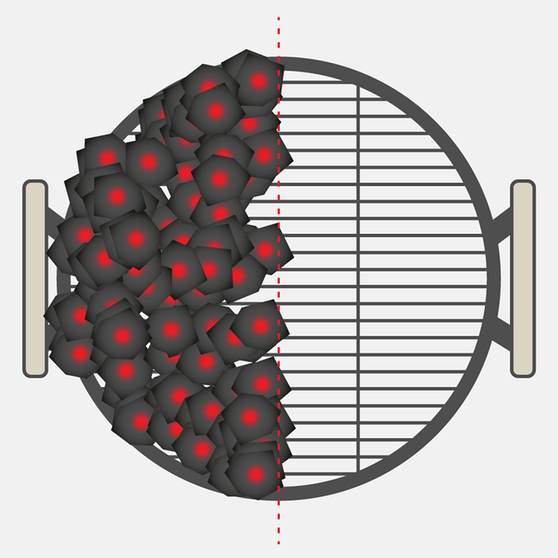
\includegraphics[width=.5\linewidth]{pics/ZweiZonen}
		\captionof{figure}{Zwei-Zonen-Glut}
		\label{fig:ZweiZonen}
	\end{minipage}%
	\begin{minipage}{.5\textwidth}
		\centering
		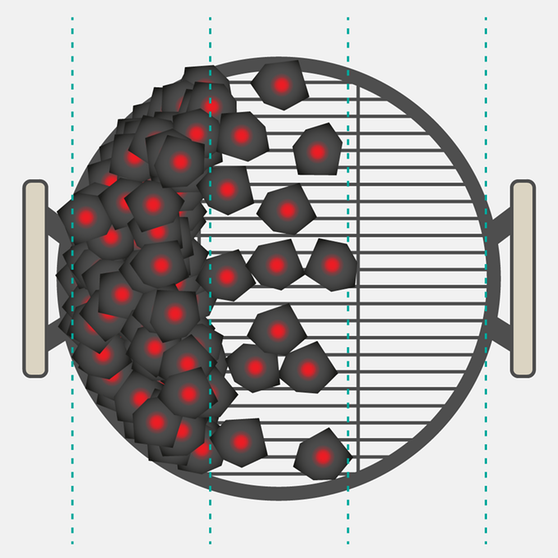
\includegraphics[width=.5\linewidth]{pics/DreiZonen}
		\captionof{figure}{Drei-Zonen-Glut}
		\label{fig:DreiZonen}
	\end{minipage}%
\end{figure}

	Für eine Drei-Zonen-Glut zu werden 2/3 des Kohlerosts mit Holzkohle oder 
	Briketts bedeckt, entsprechend der 
	Abbildung~\vref{fig:DreiZonen}. Die Glut wird am Rand so hoch gestapelt, dass 
	eine starke Hitze entsteht und fällt zur Mitte 
	hin 
	ab. So hat man am Rand eine direkte starke Hitze, in der Mitte eine direkte 
	mittlere Hitze und indirekte Hitze auf der anderen 
	Seite.

\begin{figure}[htbp]
	\centering
	\begin{minipage}{.5\textwidth}
		\centering
		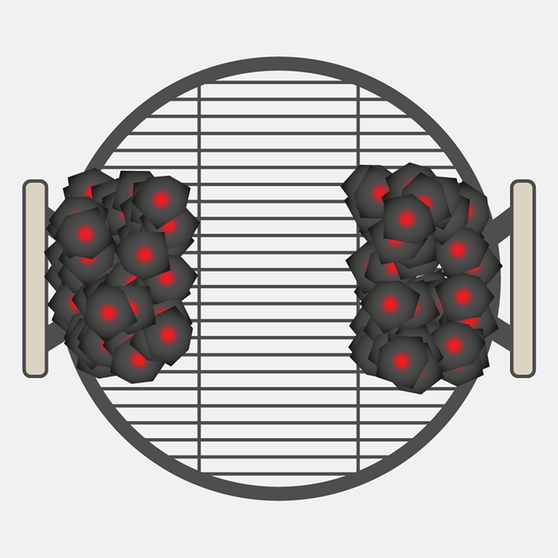
\includegraphics[width=.5\linewidth]{pics/ZweiZonengeteilt}
		\captionof{figure}{Geteilte Zwei-Zonen-Glut}
		\label{fig:ZweiZonengeteilt}
	\end{minipage}%
	\begin{minipage}{.5\textwidth}
		\centering
		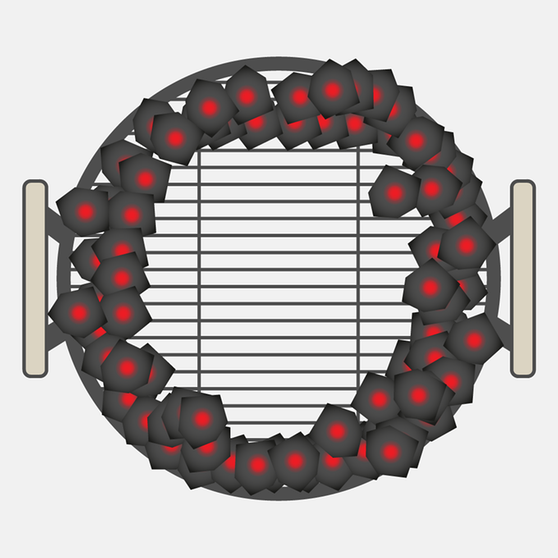
\includegraphics[width=.5\linewidth]{pics/FeuerRing}
		\captionof{figure}{Der Feuer-Ring}
		\label{fig:FeuerRing}
	\end{minipage}%
\end{figure}

	Die Methode der geteilten Zwei-Zonen-Glut, siehe 
	Abbildung~\vref{fig:ZweiZonengeteilt}, hat gleich zwei Vorzüge. Zum 
	einen verteilt sich
	die indirekte Hitze gleichmäßig zum anderen kann in der Mitte des Grills eine 
	feuerfeste Tropfschale platziert werden. Die mit 
	Wasser, Bier, 
	Fruchtsaft etc. befüllt werden kann, das aromatisiert das Grillgut, schützt es 
	vor dem Austrocknen und hält die Temperatur 
	konstant.
	
	Während die geteilte Zone für größere Braten und die Rotesserie ideal ist, ist 
	die Variante Feuer- Ring wie in 
	Abbildung~\vref{fig:FeuerRing}
	dargestellt, besonders geeignet für das berühmte Brathähnchen, das man auf 
	eine halbvolle Bierdose oder auf einen 
	Hähnchenhalter stülpt
	und im geschlossenen Grill indirekt grillt.

\begin{figure}[htbp]
	\centering
	\begin{minipage}{.5\textwidth}
		\centering
		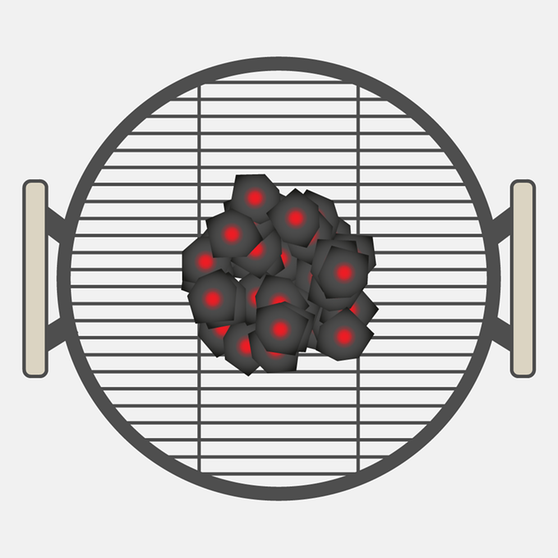
\includegraphics[width=.5\linewidth]{pics/BullsEye}
		\captionof{figure}{Das Bulls Eye}
		\label{fig:BullsEye}
	\end{minipage}%
	\begin{minipage}{.5\textwidth}
		\centering
		\includegraphics[width=.5\linewidth]{pics/MenionRIng}
		\captionof{figure}{Der Menion-Ring}
		\label{fig:MenionRing}
	\end{minipage}%
\end{figure}

	Das Bulls Eye ist das Gegenteil des Feuer-Rings, siehe 
	Abbildung~\vref{fig:BullsEye} und ist bestens geeignet für 
	Kurzgebratenes. Der Grill
	sollte dafür aber groß genug sein um eine indirekte Zone entsprechender 
	Größe zu bekommen.
	
	Der ">heilige Gral"< des indirekten Grillens ist der Menion-Ring, siehe 
	Abbildung~\vref{fig:MenionRing}. Richtig angewendet, 
	kann man damit
	im geschlossenen Grill bis zu 20 (!) Stunden indirekt bei knapp 120°C grillen, 
	ohne Briketts nachlegen zu müssen. Briketts 
	zweireihig anordnen. 
	Die Briketts müssen sich unbedingt berühren. Die Starterbriketts (weiß im Bild) 
	bereitet man im Anzündkamin vor (zur Hälfte 
	füllen), sie werden
	an den Rand des Rings platziert. So glüht der komplette Ring Stück für Stück 
	durch. Ideal z. B. für ">The holy trinity of BBQ"< 
	\ bestehend aus 
	Beef Brisket, Pulled Pork und Spareribs.

\subsection{Handhabung des Holzkohlegrills}

	Ein Holzkohlegrill kann mit Holzkohle oder Briketts (ich werde im weiteren 
	Verlauf nur von Holzkohle reden, Briketts sind im 
	gleichen Maße 
	betroffen) beheizt werden. 
	Der Unterschied liegt an der Hitze und der Brenndauer. Die Holzkohle brennt in 
	der Regel heißer, die Briketts dagegen länger. 
	Die Entscheidung welches Medium genutzt wird ist keine reine 
	Geschmackssache, sondern auch zum Teil des Grillgutes 
	gewidmet. Dazu später 
	mehr.

	\paragraph{Methoden des Anfeuern}

	Es gibt verschiedene Arten den Grill anzufeuern, zum Einen gibt es die 
	Möglichkeit die Holzkohle respektive die Briketts auf 
	dem Grillrost,
	entsprechend der gewünschten Heizzonen wie in Abschnitt~\vref{Heizzonen} 
	erklärt, anzurichten. Dann die Holzkohle mit 
	einem flüssigen oder 
	festen Grillanzünder
	an zu zünden. Diese gibt es sowohl mit Paraffin und/ oder Petroleum oder 
	schadstoffe frei. Hat man welche aus Paraffin oder 
	solche die Petroleum 
	beinhalten, muss auf eine 
	vollständige Verbrennung der Grillanzünder geachtet werden.
	
	Dann gibt es die Möglichkeit die angerichtete Holzkohle mit einem Heißluftföhn 
	zu erhitzen. Dabei ist man allerdings auf eine 
	Stromquelle 
	angewiesen, was sich m.E. als Nachteil
	erweisen kann.
	
	Als weitere Möglichkeit gibt es die elektrischen Grillanzünder, die an einen 
	Tauchsieder erinnern. Diese werden zwischen die 
	Kohlen gelegt und an 
	eine Steckdose angeschlossen. 
	Innerhalb weniger Minuten ist die Holzkohle durchgeglüht. Auch dabei ist eine 
	Stromquelle nötig.
	
	Meine präferierte Methode ist der Anzündkamin.  Darin wird die Holzkohle 
	aufgeschichtet und mit einem Grillanzünder 
	angezündet. Ich benutze 
	Anzünder aus gewachster Holzwolle. 
	Oder ein ölgetränktes Blatt von der Küchenrolle, mit dem ich den Grillrost leicht 
	eingefettet habe. Die Holzkohle glüht von unten nach oben 
	durch, mit Hilfe der 
	Luft die wie in einem Kamin von unten nach oben steigt
	und den wichtigen Sauerstoff transportiert. Ist die Holzkohle durchgeglüht, 
	man erkennt es an der grauen Asche auf den 
	Kohlestücken, wird die 
	Kohle in den Grill geschüttet und 
	entsprechend der gewünschten Heizzone arrangiert.

	\paragraph{Reinigen nach dem Grillen}

	Nach dem Grillen ist in der Regel noch genug Hitze im Grill um den Rost 
	nochmal auf Temperatur zubringen, dass die Reste 
	des Grillguts 
	weitestgehend verbrennen. 
	Mit einer Messingdrahtbürste kann dann der Rost abgebürstet werden.
	
	Sobald der Grill abgekühlt und die Glut vollständig erloschen ist, sollte die 
	Asche entfernt werden. Da die Asche 
	hygroskopisch ist und Wasser 
	selbst aus 
	der Luft anzieht. Durch die Feuchte die sich in der Asche bildet kommt es nach 
	einiger Zeit zur Rostbildung. Das wird durch 
	entfernen der Asche 
	vermieden.
	Weitere Reinigung ist nicht notwendig, es sei den der Grill ist sehr stark 
	verschmutzt und es haben sich schon relativ dicke 
	Anbackungen 
	entwickelt.
	Die Anbackungen können mit einer Holzspachtel, die beim Raclette verwendet 
	wird, abgeschabt werden.
	
	
		\begin{figure}[htbp]
		\centering
		\begin{minipage}{1\textwidth}
			\centering
			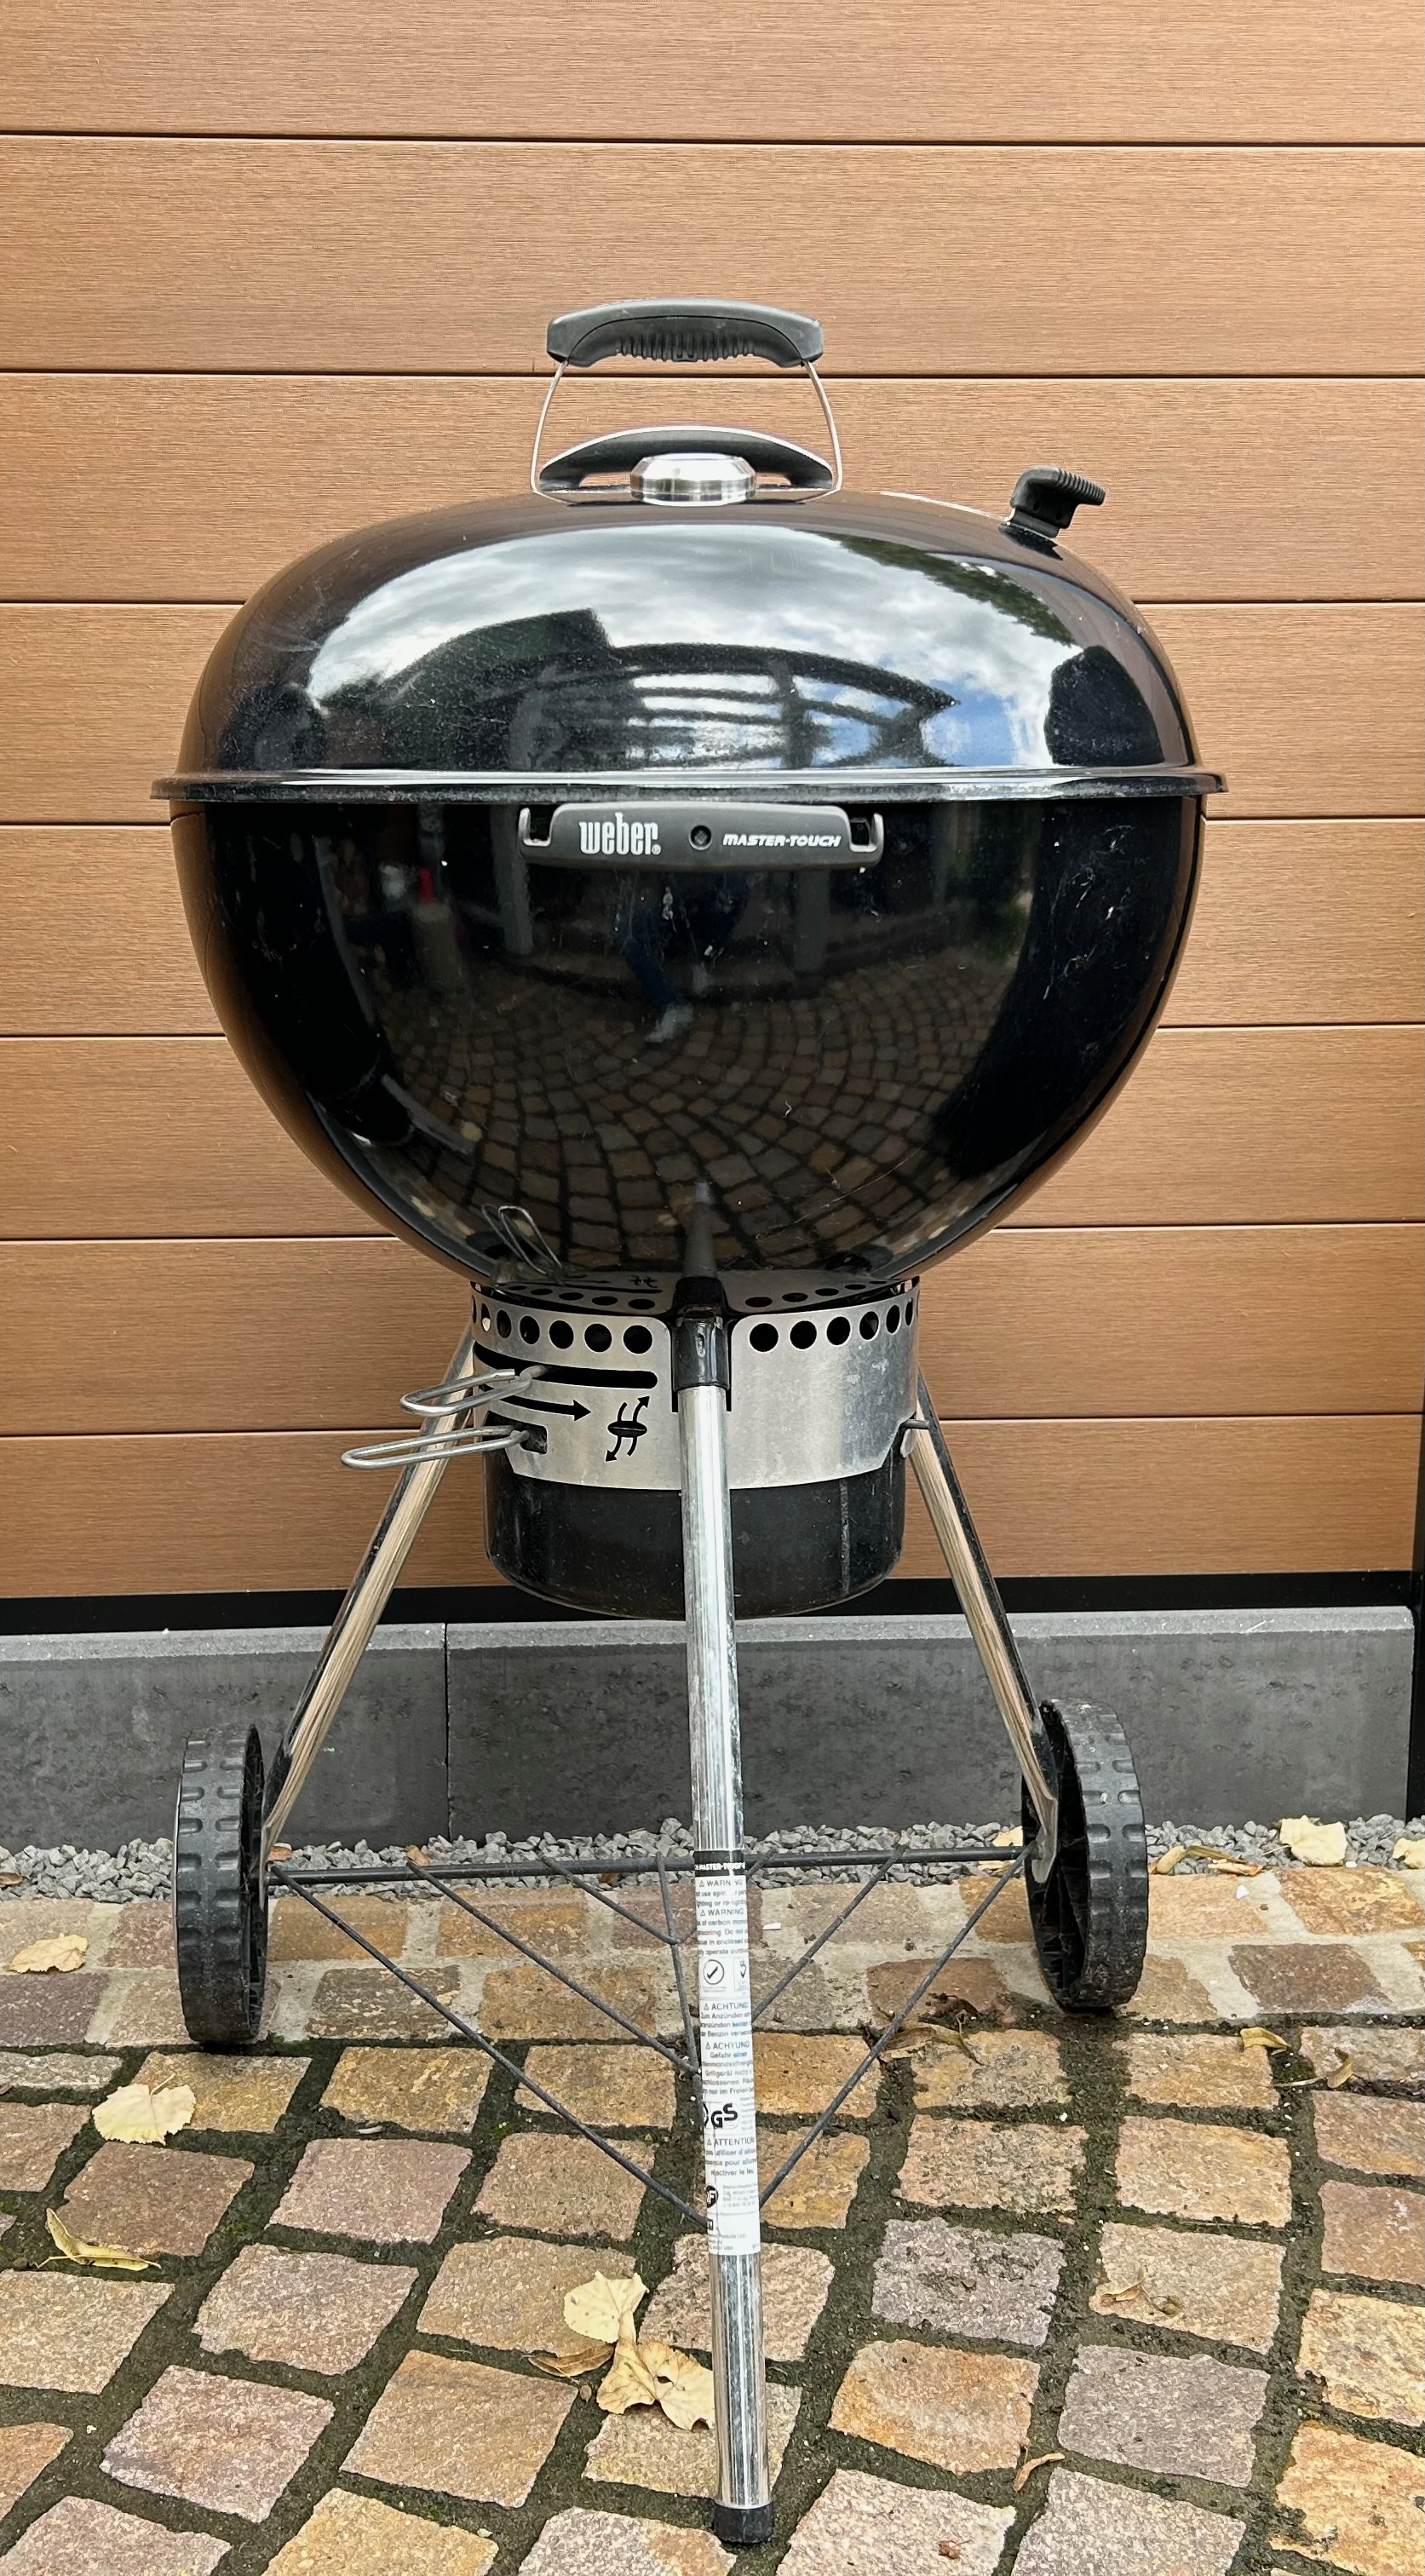
\includegraphics[width=.6\linewidth]{pics/Kugelgrill}
			\captionof{figure}{Kugelgrill Weber One Touch}
			\label{fig:Kugelgrill}
		\end{minipage}%
	\end{figure}
	
	\newpage

\section{Der Kamado Grill}

	Das Prinzip des Keramik-Grills ist bereits mehrere tausend Jahre alt. Es begann 
	mit einem Loch, das 
	mit Steinen, später mit Lehm und Ton ausgekleidet und als weitere Entwicklung 
	mit 
	einem Rand versehen wurde um das Feuer vor Wind zu schützen. 
	Im Laufe von einigen tausend Jahren wurde in der Edo-Zeit in Japan (Anfang 
	des 17ten Jahrhunderts 
	bis Mitte des 19ten Jahrhunderts) aus dem Feuerloch der Mushi-Kamado, die 
	heutige Form
	der Kamado-Grills.
	
	Im Nachkriegsjapan wurde von einem in Japan stationierten Amerikaner, dieser 
	Reis-Dampfgarer mit 
	einem Rost zum Grill umgebaut. Mit den Amerikanern kam dieser ">Grill"< nach 
	Amerika und begann 
	einen Siegeszug um die Welt. Über den Teich kam der Grill erst um das 
	Millennium herum, als 
	Kochgerät für die Spitzengastronomie (vorrangig in Belgien und der 
	Niederlande). Der Keramik-Grill (siehe Abbildung ~\vref{fig:Keramikgrill}) ist heute
	auch für grillbegeisterte Privatleute erschwinglich und in der Regel nur ein paar 
	Mausklicks und 
	mehrere Hundert bis wenige tausend Euro entfernt.
	
	Der Keramik-Grill ist eiförmig und wird mit einen Gestell, das Nest genannt 
	wird, geliefert. Falls der 
	Einbau in eine Außenküche gewünscht ist, kann er auch ohne Gestell geliefert 
	werden.
	Da die Grills aus Keramik bestehen werden sie im fernen Osten, genau 
	genommen China, das über 
	eine mehre tausend Jahre alte Tradition der Keramikverarbeitung verfügt, 
	gefertigt. Es gibt 
	verschiedene Hersteller von Keramik-Grills, die Big-Player in diesem Segment 
	sind Big Green Egg, 
	Kamodo Joe und Monolith . Die beiden erstgenannten sind amerikanische 
	Unternehmen, ohne in 
	überschwänglichen Patriotismus zu verfallen ist meines Erachtens der Monolith 
	im Augenblick der am 
	Besten durchdachte Keramik-Grill im Kreis der Big-Player. Der niederländische 
	Hersteller IQ liefert 
	mehr Zubehör mit, kann allerdings nicht mit den drei genannten Marken mit 
	halten. Entgegen der 
	landläufigen und von den Herstellern propagierten Meinung die Keramik spiele 
	eine große Rolle, ist 
	dem nicht so. Punkten können die verschiedenen Hersteller nur mit dem 
	Zubehör, der mehr oder 
	weniger gut durchdacht ist, oder eben Funktionen die die Mitbewerber nicht 
	oder nicht in der Qualität 
	anbieten. So verfügt der Monolith über das beste Rostsystem, das beste 
	System zur Einbringung von 
	Räucher-Chips und Asche-Entnahme-System. Des Weiteren ist ein eingebauter 
	Adapter für den BBQ-
	Guru angebracht. Als Kritikpunkt kann gesagt werden, dass das Nest kein 
	Design-Highlight darstellt.
 
\subsection{Handhabung des Kamado-Grills}

	Die Handhabung des Kamado-Grills unterscheidet sich in wenigen Punkten 
	zum Kugelgrill. Im Kamado-
	Grill werden die indirekten Zonen in der Regel über zwei halbkreisförmige 
	Deflektorsteine realisiert. 
	Das heißt es werden keine Heizzonen durch die Lage der Holzkohle 
	eingerichtet. Bei dem Monolith Pro Serie ist
	es möglich den Grillkorb zu unterteilen und den Korb nur halb mit Kohle 
	zufüllen. Durch die Teilbaren 
	Roste und Deflektorsteine können auch auf diese Weise direkte und indirekte 
	Zonen eingerichtet 
	werden.
	Der nächste Unterschied ist, dass der Deckel im Betrieb nur einen Spalt weit 
	geöffnet werden darf bis 
	ein Luftaustausch stattgefunden hat und der Grill komplett geöffnet werden 
	kann. Bei zu schnellem Öffnen kann es durch den einströmenden 
	Sauerstoff zu einem Flammenschlag kommen. Daher besteht ein gewisses 
	Verletzungsrisiko.

\subsection{Anfeuern des Kamado-Grills}

	Es wird empfohlen eine Holzkohle, die frei von chemischen Zusatzstoffen ist zu 
	verwenden. Die Holzkohle
	sollte eine homogene Größe der Kohlestücke haben und außerdem großstückig 
	sein. Briketts sind für Keramikgrill
	nicht zu empfehlen, da sie Bindemittel enthalten, die sich in der Keramik 
	festsetzen. Außerdem ist die
	Hitze der Briketts zu gering für den Keramik-Grill.
	
	Hier eine Auflistung der Bindemittel die in Briketts eingesetzt werden.

	\begin{itemize}[noitemsep]
		\item Stärke
		\item Ton
		\item Melasse
		\item Holzteer
		\item Pech
	\end{itemize}
 
  
	Bei einem Longjob wie z.B. Beef Brisket, Pulled Pork oder Spare Ribs wird der 
	Feuerkorb befüllt. Der 
	Feuerkorb kann mehr Kohle aufnehmen als der  Kohlekorb. Bei kürzeren 
	Garzeiten, aber höheren 
	Temperaturen sollte der Kohlekorb eingesetzt werden. Da weniger Kohle 
	benötigt wird. Bedingt durch 
	den Kohlekorb wird die Holzkohle optimal mit Sauerstoff versorgt.
	Angefeuert werden kann der Grill mit Bio-Anzündern. Wenn schnell eine hohe 
	Hitze, siehe 
	Abbildung~\vref{fig:Große}, erreicht werden soll, werden 3 Anzünder benötigt. 
	Die in einem Dreieck auf 
	die Kohle gelegt und angezündet werden. Die Be- und Entlüftung wird komplett 
	geöffnet.
	
	Bei geringer Hitze wird nur ein Grill-Anzünder benötigt. Auch hier werden die 
	Lüftungsschlitze ganz 
	geöffnet. Bevor der Grill die Wunschtemperatur erreicht, sollte der Grill durch 
	schließen der 
	Lüftungsschlitze (bitte nicht ganz, da sonst das Feuer erstickt) abgefangen 
	werden. Das Abkühlen eines 
	Kamado-Grills dauert, durch die hohe Wärmekapazität der Keramik, sehr lange.
	
	Alternativ zu den Grillanzündern kann auch ein Looftlighter zum Entzünden der 
	Holzkohle verwendet 
	werden. Ich benutze einen Heißluftföhn, der für das Anzünden von Grillkohle 
	geeignet ist.

\begin{figure}[htbp]
	\centering
	\begin{minipage}{.5\textwidth}
		\centering
		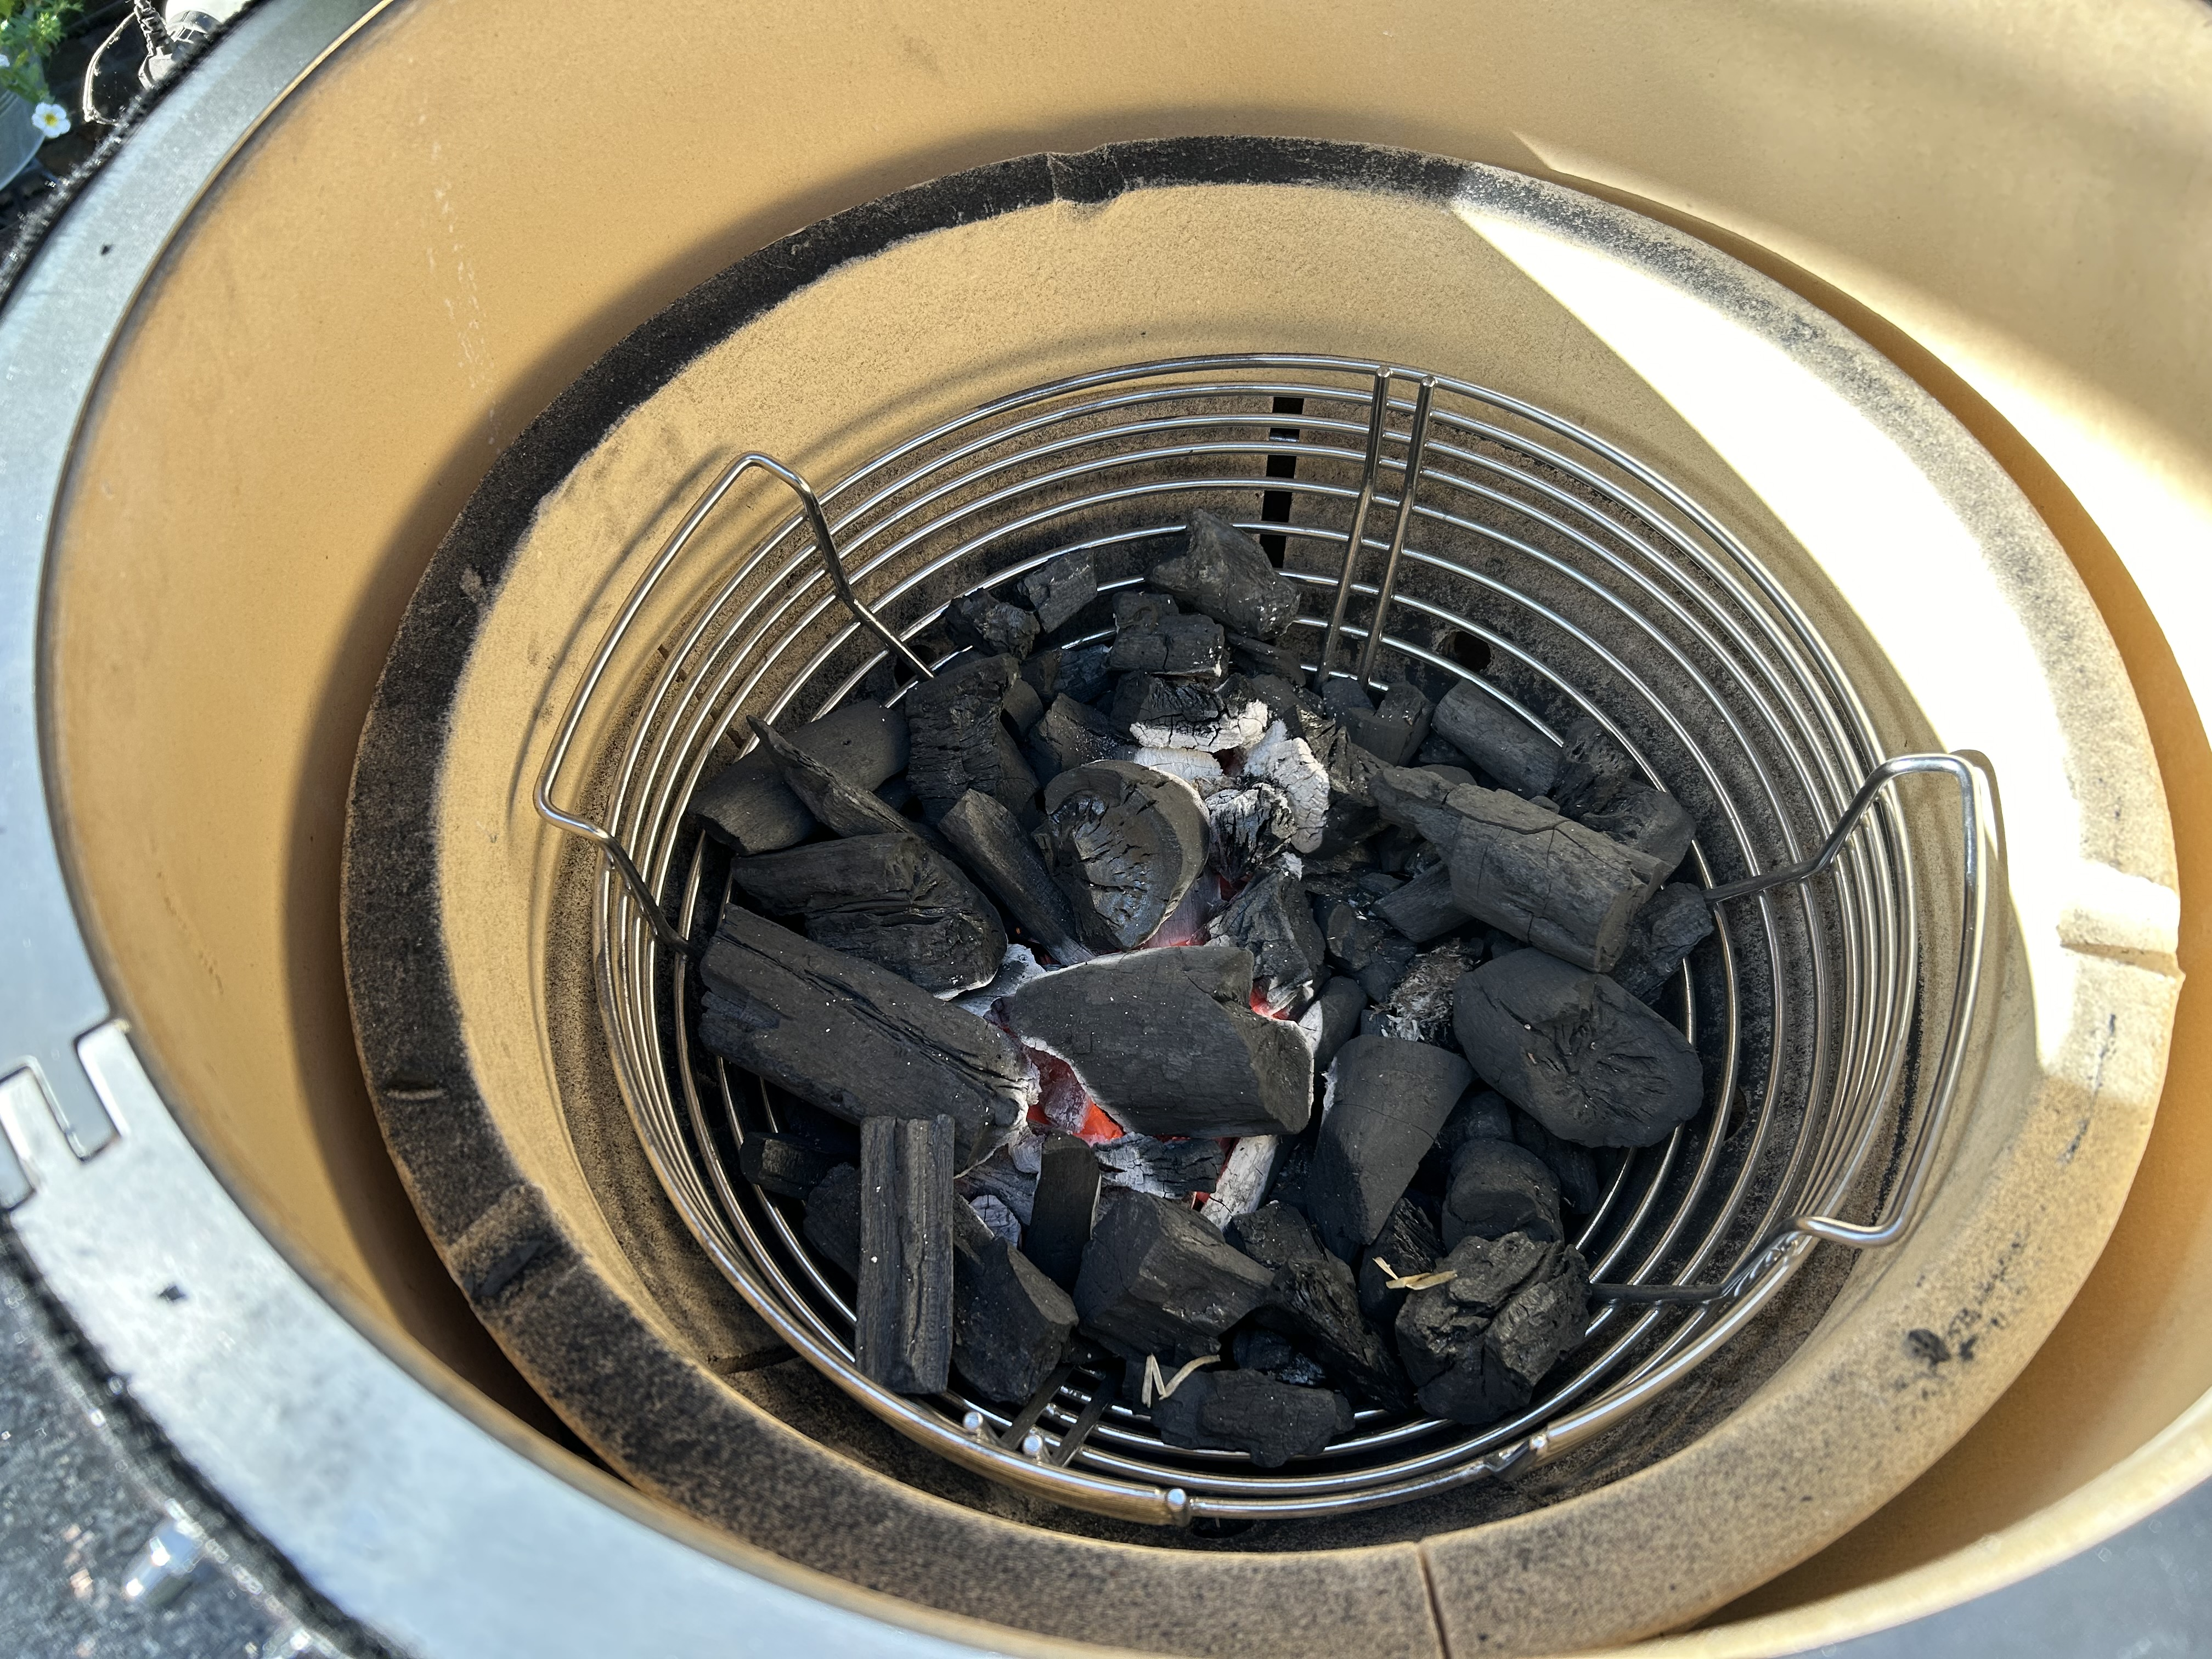
\includegraphics[width=.5\linewidth]{pics/Anfeuern_Monolith}
		\captionof{figure}{Anfeuern Monolith}
		\label{fig:Anfeuern}
	\end{minipage}%
	\begin{minipage}{.5\textwidth}
		\centering
		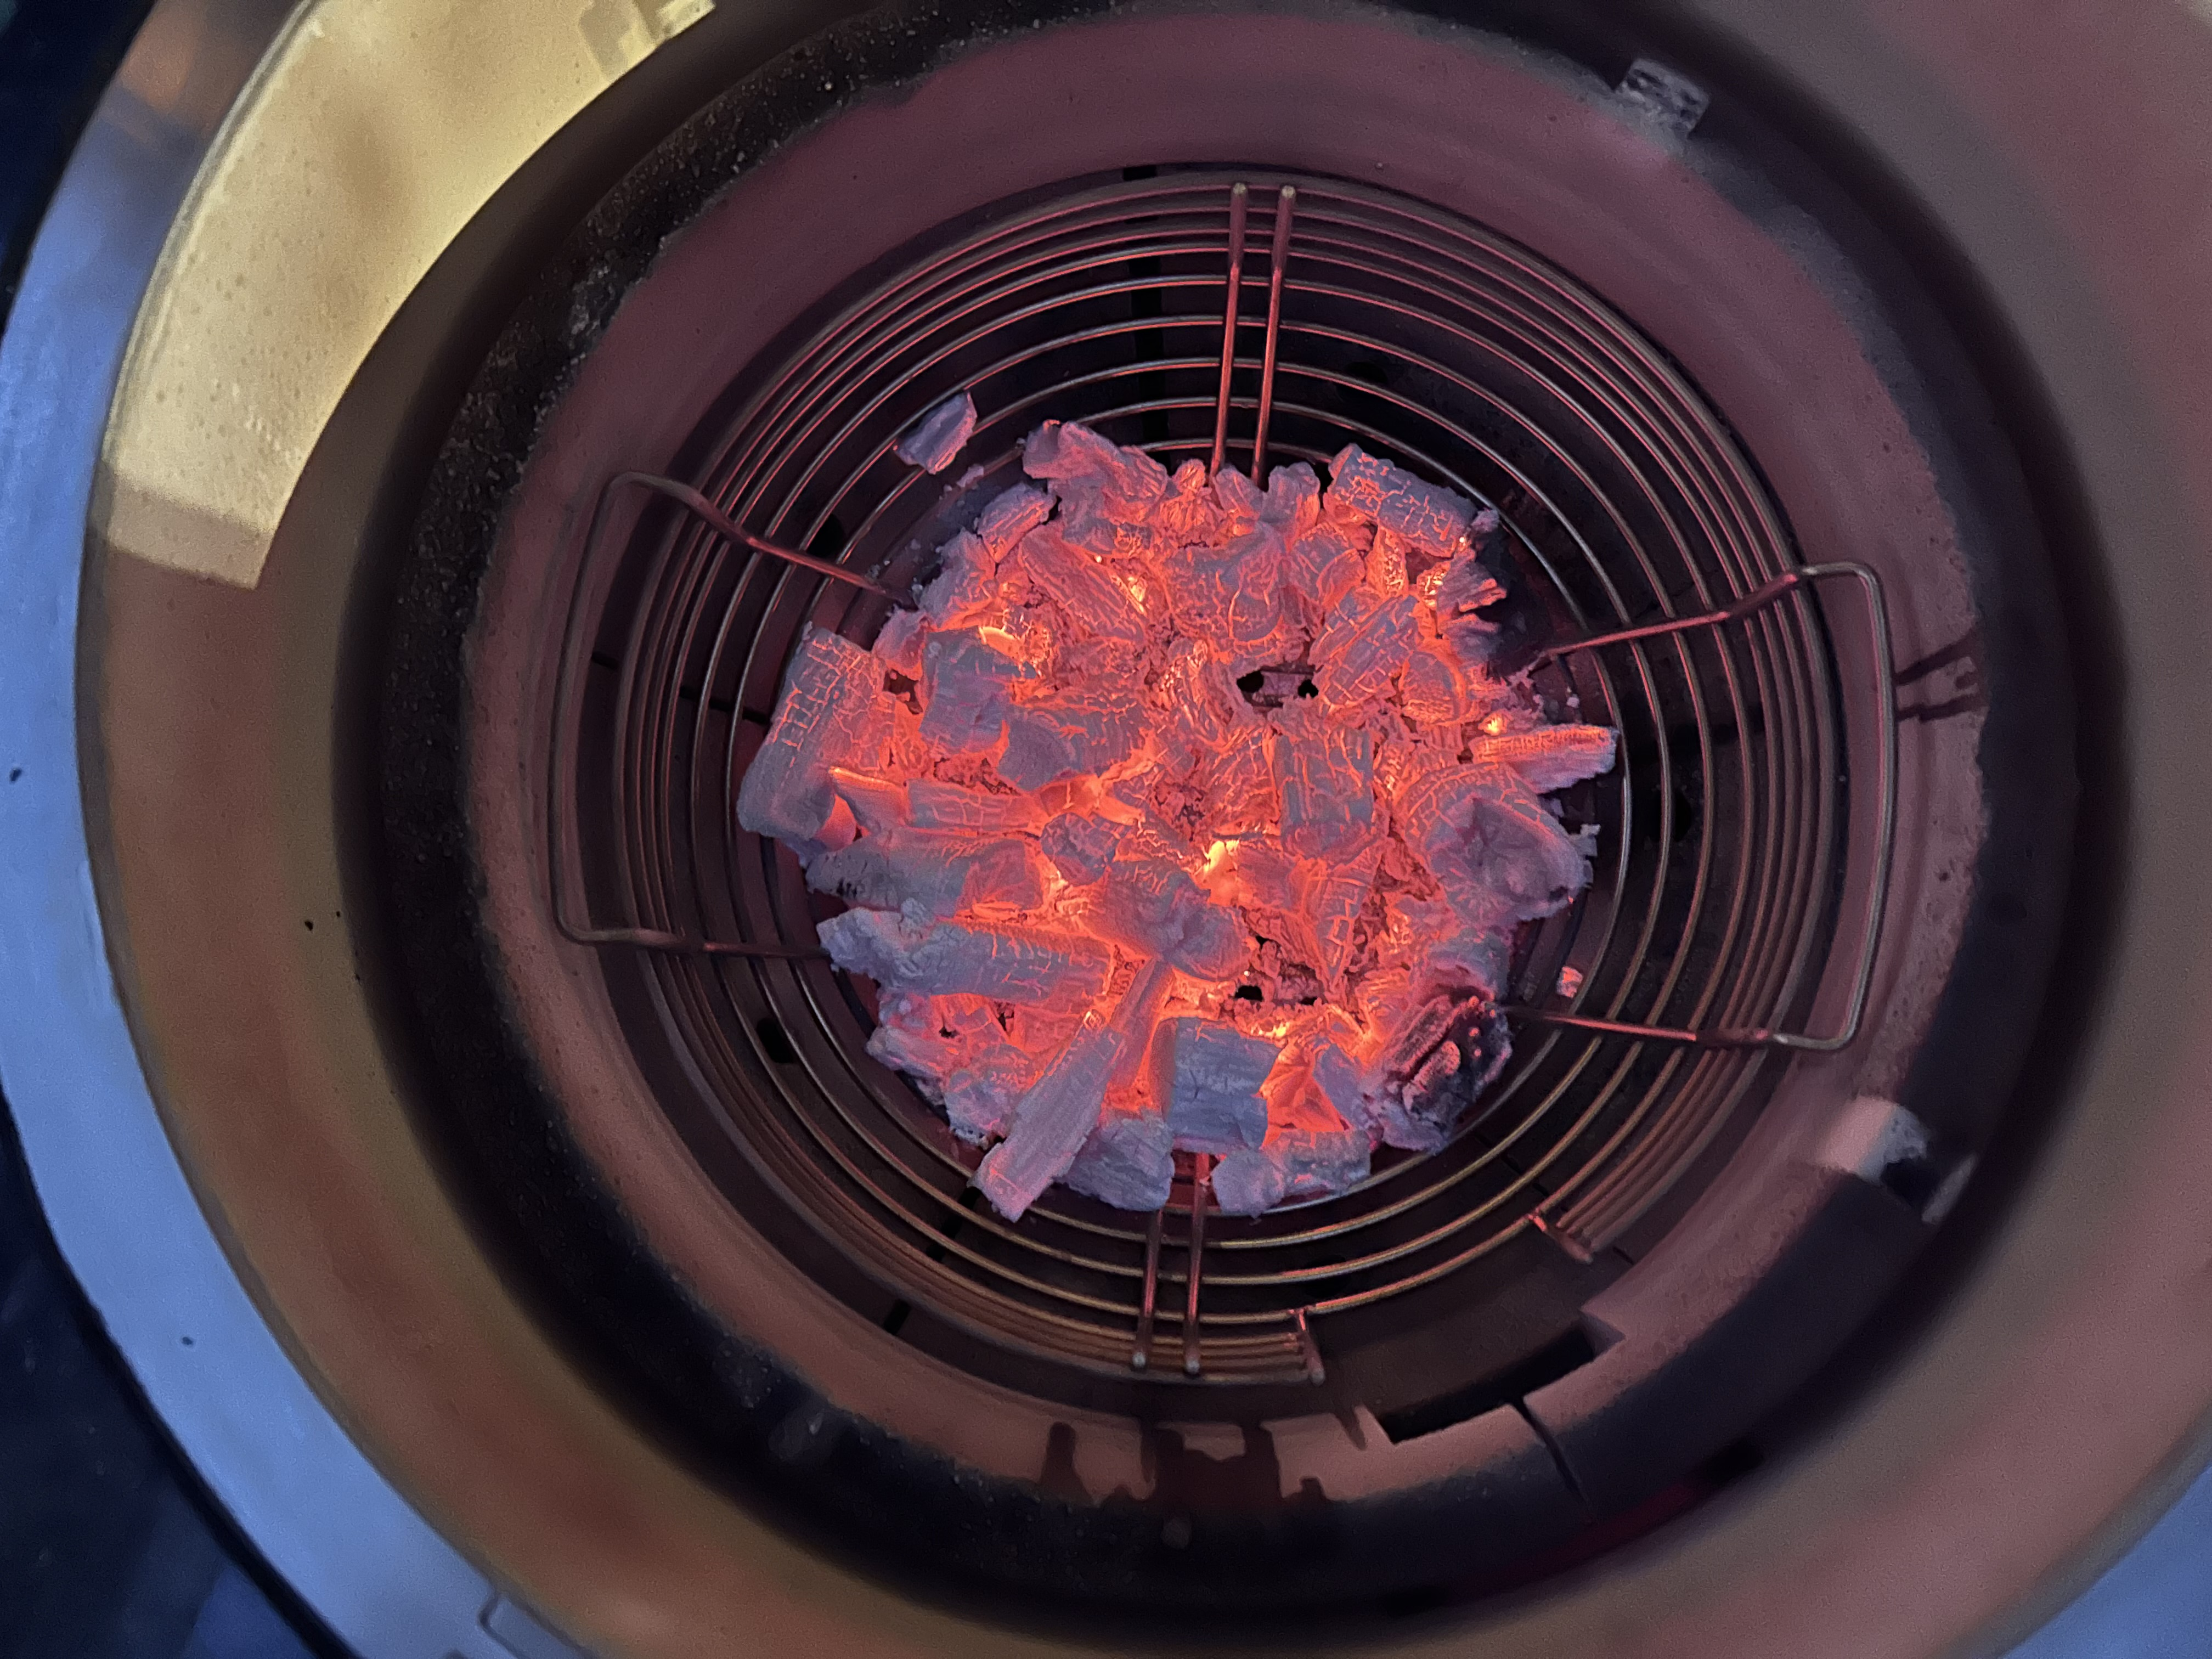
\includegraphics[width=.5\linewidth]{pics/Große_Hitze}
		\captionof{figure}{Große Hitze}
		\label{fig:Große}
	\end{minipage}%
\end{figure}
\newpage

\subsection{Reinigen des Kamado-Grills}

	Das Reinigen erfolgt durch Aufheizen und Abbürsten der Roste und spülen der 
	Abtropfwannen. Die 
	Reinigung der Keramik erfolgt durch starkes Erhitzen (Pyrolyse bei ca. 400°C).
	
	\begin{figure}[htbp]
		\centering
		\begin{minipage}{1\textwidth}
			\centering
			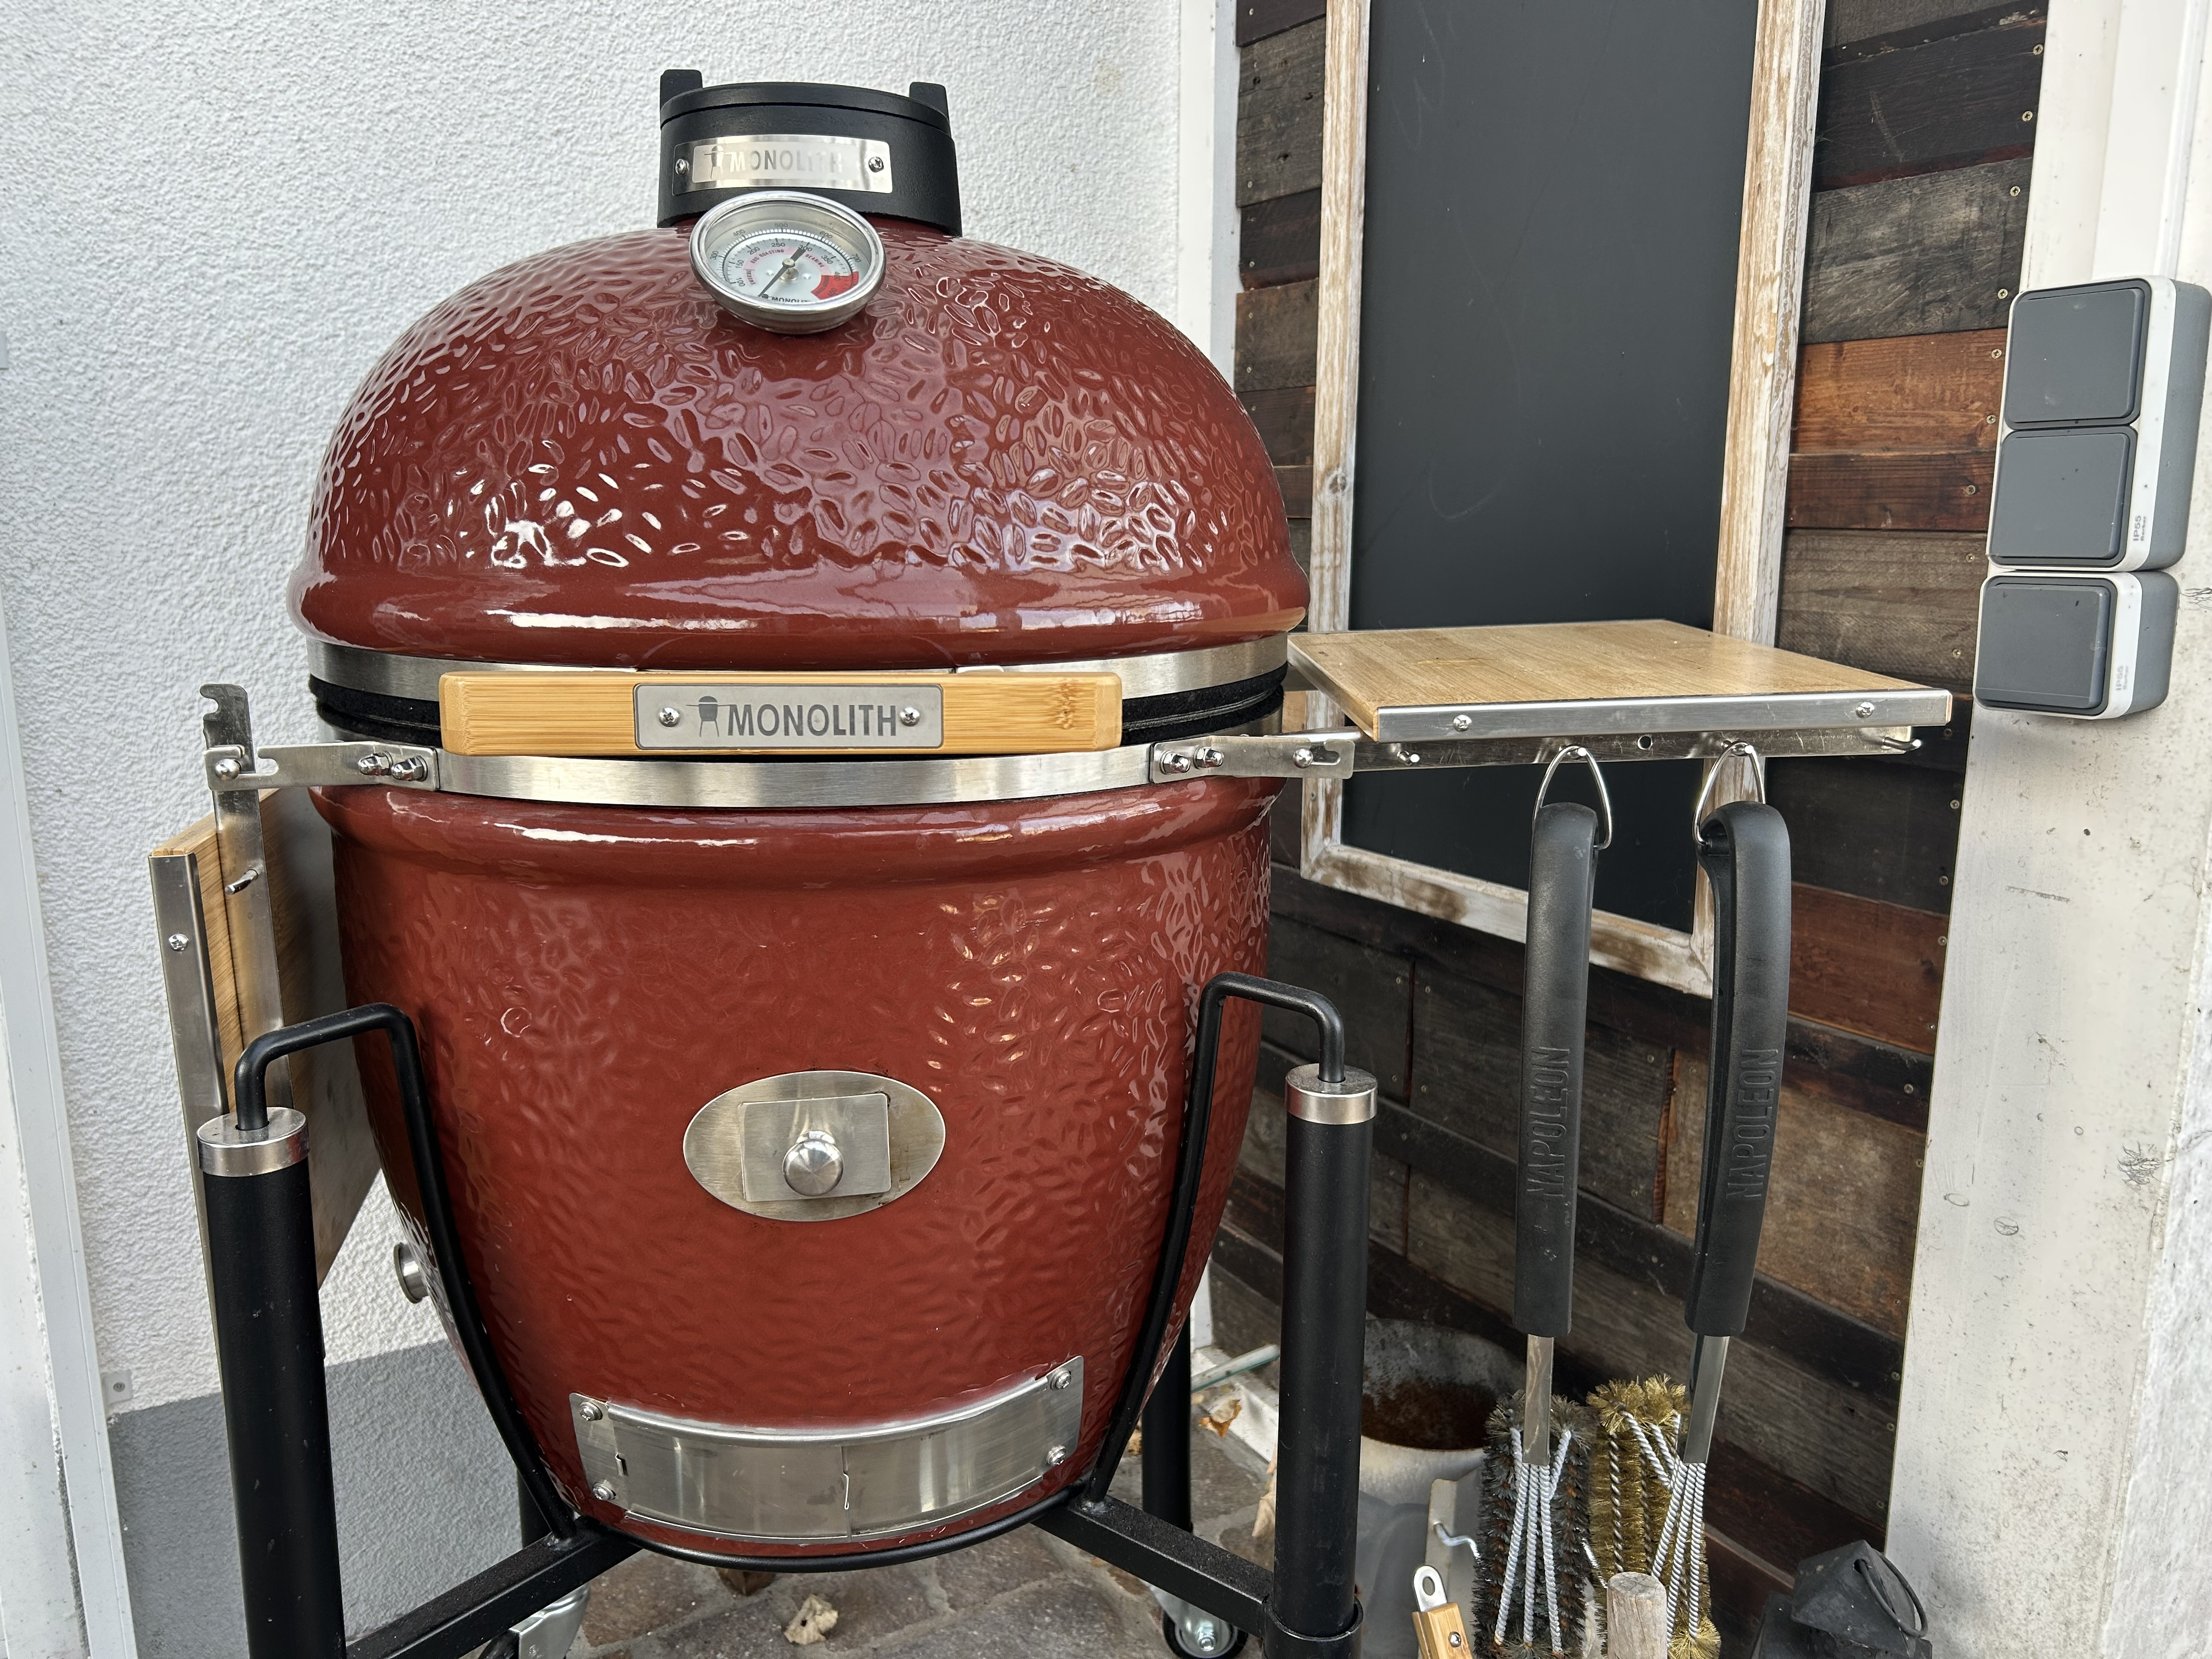
\includegraphics[width=1\linewidth]{pics/Keramikgrill}
			\captionof{figure}{Kamado-Grill Monolith Classic 2 Pro}
			\label{fig:Keramikgrill}
		\end{minipage}%
	\end{figure}
\newpage
\section{Der Gasgrill}

	Die Modellvielfalt und die Ausstattungsvarianten der Gasgrills ist gefühlt noch 
	umfangreicher als bei den 
	Holzkohle-Grills. Es gibt Gasgrills die für 
	deutlich unter 100 €\ zu haben sind. Und den Oberklassengrills, die 
	hochmodern, aus bestens 
	verarbeiteten und qualitativ hochwertigen Materialien
	hergestellt sind und preislich jenseits der 15.000~€\ liegen. Dazwischen gibt es 
	Gasgrills in allen 
	erdenklichen Ausstattungsvariationen, Qualitätsstufen und Preisklassen. 
	

\subsection{Was benötige ich bei einem Gasgrill unbedingt?} 

	Hier ist die 
	Antwort gar nicht so leicht. 
	Es kommt auf die Ansprüche an. Habe ich 
	vor mich mit dem Grillen intensiver zu beschäftigen komme ich um indirektes 
	Grillen nicht herum. In diesem Fall sind 
	mindestens drei Hauptbrenner 
	Pflicht.  Bei zwei Brennern ist der Abstand von der indirekten Grillfläche zu der 
	direkten Grillfläche zu klein. Besser ist ein Grill 
	mit vier 
	Hauptbrennern. Ich persönlich besitze einen Grill mit drei Hauptbrennern, 
	einem Seitenkochfeld siehe Abbildung~\vref{fig:Napoleon}und einem Heckbrenner. Da 
	ich einen 
	Oberflächengrill mit einer Maximaltempera~tur von 800°C besitze, konnte ich 
	mir den Keramikbrenner in meinem Gasgrill 
	sparen. 
	
	Sollte der Gasgrill nicht ausreichen, zum Beispiel für ein Beef Brisket Full 
	Packer, nehme ich den Kugelgrill oder den Smoker 
	zur Hand. Aus diesem 
	Grund musste der Gasgrill nicht sehr groß dimensioniert sein. 
	
	Eine Schlauchbruchsicherung, die gegen ausströmendes Gas schützt, ist 
	meines Erachtens für die Sicherheit unerlässlich 
	und sollte unbedingt nachgerüstet 
	werden. 
	Auch bei hochwertigen Grills im gehobenen Preissegment sind 
	Schlauchbruchsicherungen siehe 
	Abbildung~\vref{fig:Sicherung} so gut wie nicht im 
	Lieferumfang enthalten. Dieses Bauteil ist für kleines Geld, ca. 13,00 € bis 
	20,00~€, erhältlich. Die Sicherheit des Grillers 
	oder umstehenden 
	Personen sollte diese geringe Investition wert sein. Im 
	professionellen Bereich ist so ein Bauteil gesetzlich gefordert.

\begin{figure}[htbp]
	\centering
	\begin{minipage}{.5\textwidth}
		\centering
		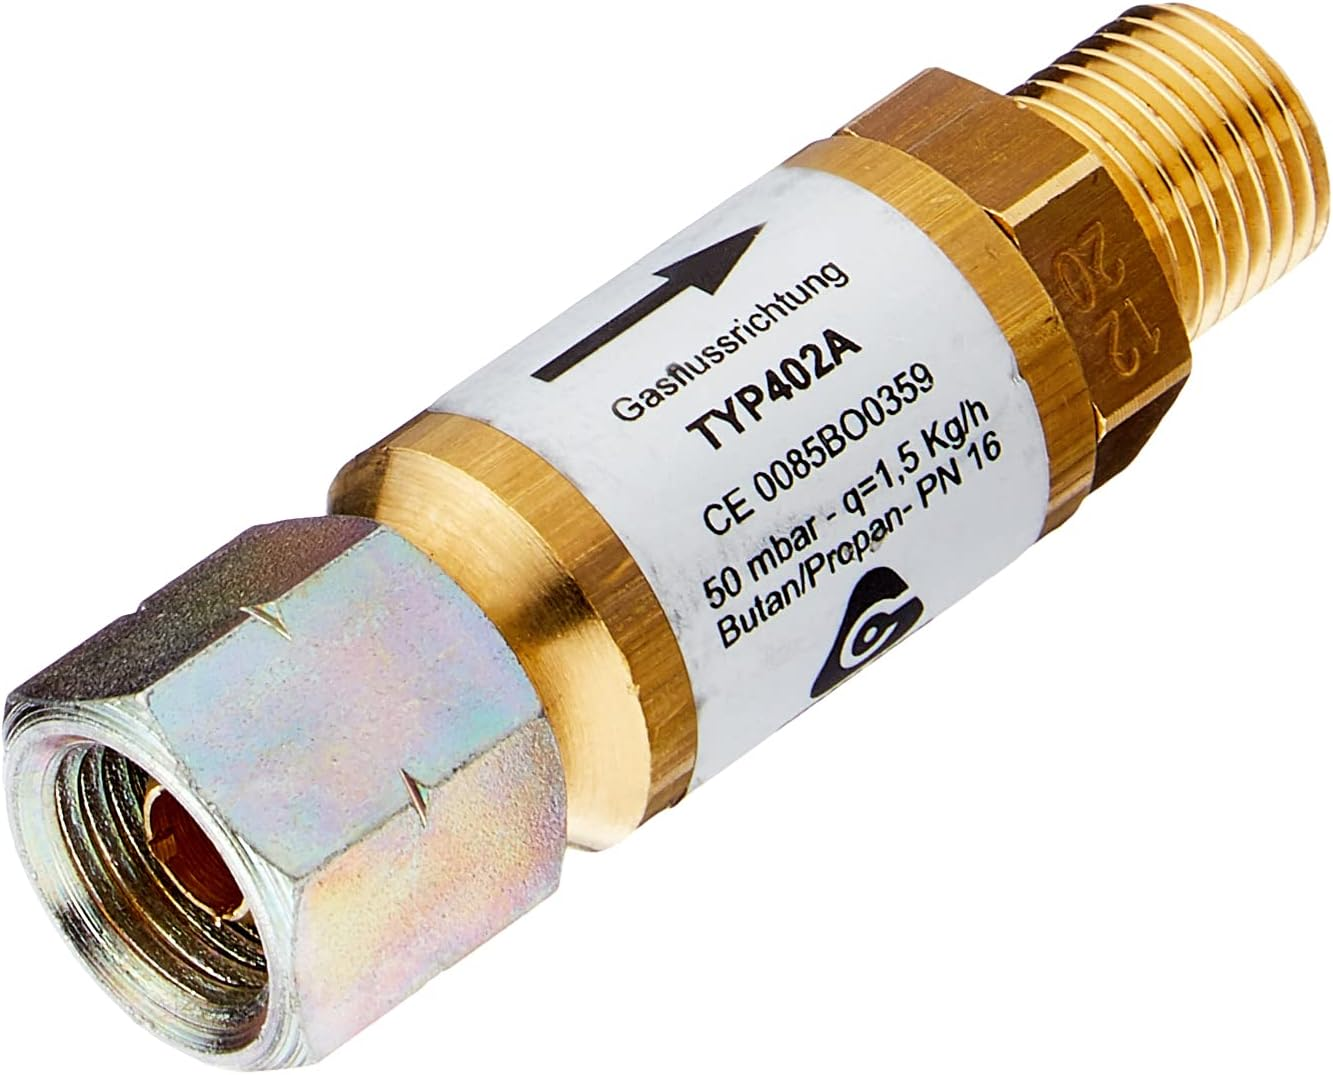
\includegraphics[width=.5\linewidth]{pics/Schlauchbruchsicherung}
		\captionof{figure}{Schlauchbruchsicherung}
		\label{fig:Sicherung}
	\end{minipage}%
	\begin{minipage}{.5\textwidth}
		\centering
		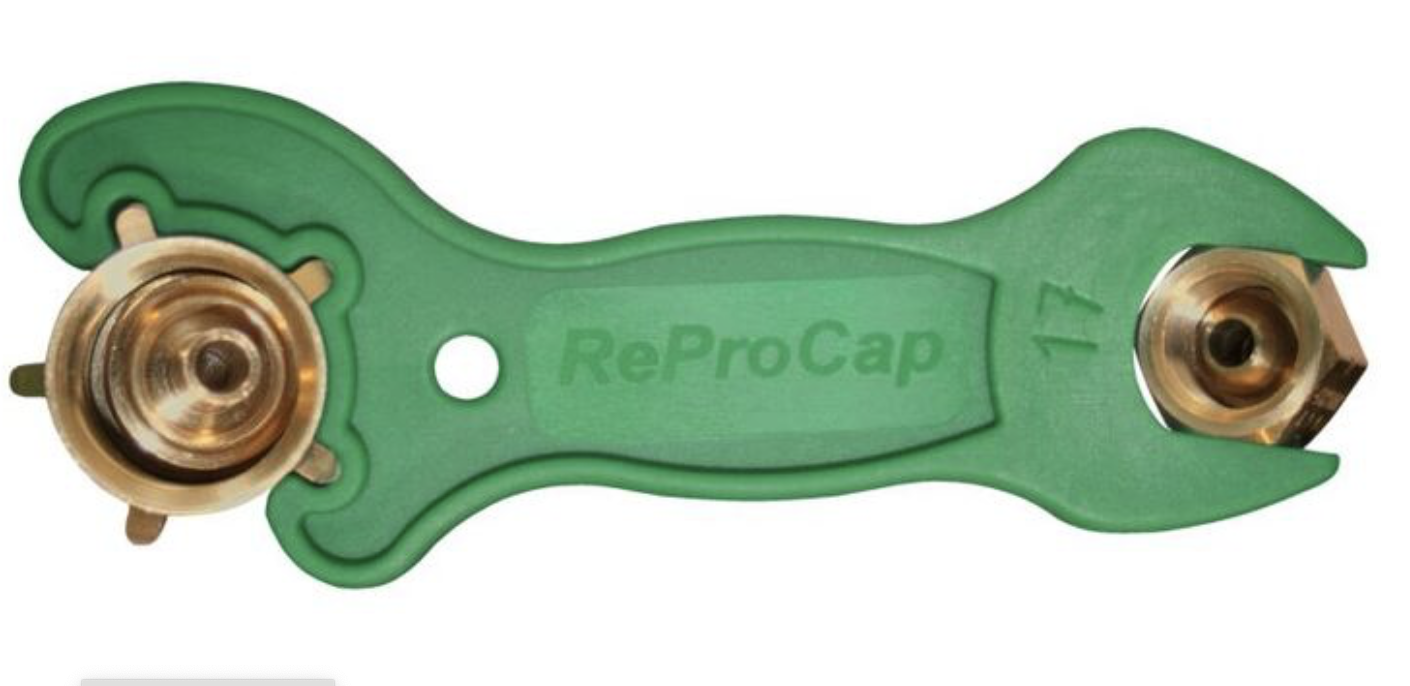
\includegraphics[width=.5\linewidth]{pics/Schlüssel}
		\captionof{figure}{Schlüssel}
		\label{fig:Schlüssel}
	\end{minipage}%
\end{figure}

\subsection{Woran erkenne ich eine gute Qualität?}

	Ich achte immer auf ein paar wenige Merkmale, diese müssen zu meiner 
	Zufriedenheit erfüllt sein, damit ich mich näher mit den Grill beschäftige. 

	\begin{itemize}[noitemsep]
		\item Der Grillrost sollte aus mindestens 6mm starken Edelstahl oder 
	    5mm Gusseisen bestehen. Bei Grillrosts mit 
		geringeren Stärken
		ist es nicht ausgeschlossen, dass sie sich aufgrund der Hitze verformen.
		\item Die Drehgriffe müssen stabil in der Hand liegen, leichtgängig sein und 
		dürfen nicht wackeln. Nichts ist ärgerlicher, als ein Drehgriff, der 
		in seiner Funktion eingeschränkt ist.
		Zum Einem weil die Befestigung unzureichend ist und Griff immer abfällt. 
		Zum Anderen wenn die Kardanwelle nicht mitgenommen wird, weil 
		der Lock beschädigt ist.
		\item Der Deckel sollte schwer ausgeführt und die Scharniere leichtgängig 
		und gut ausbalanciert sein. Bei höherwertigen Grills ist der 
		Deckel doppelwandig, hier sollten auch die
		Seitenteile doppelwandig sein. In der Preisklasse des Napoleon Rogue SE 
		oder XT ist dieses Feature nicht vorgesehen. Der Deckel kann 
		allerdings für kleines Geld gepimt werden. Außerdem sind Reflektoren, die 
		unter den Brennern angebracht werden können eine sinnvolle Ergänzung 
		um die Hitze dort zu halten, wo sie gebraucht wird, in der Grillkammer.
		\item Eine 11kg Gasflasche sollte verwendet werden können. Darf nur die 
		5kg-Gasflasche verwendet werden, obwohl genug Platz für eine 
		11kg-Flasche vorhanden ist,
		ist die Abschirmung nicht stark genug. Auch das ist ein Sicherheits- und 
		Qualitätsmerkmal.
	\end{itemize}

	Eine Kaufberatung und Informationen über die Qualität von Gasgrills bekommt 
	Ihr auf dieser 
	\url{https://www.youtube.com/watch?v=4cMuaoBGZGM }\ {Webseite}

\subsection{Sicheres Handling des Gasgrills} 

	ist nicht selbstverständlich. 
	Hier ein paar Tipps wie man sich auf die 
	sichere Seite stellt. 
	Gasverpuffungen sind nicht so schnuckelig wie sich das Wort Verpuffung 
	anhört. Ganz in Gegenteil, die sind äußerst 
	gefährlich. Deshalb habe ich 
	den Abschnitt auch aufgenommen. Wenn ich euch nix Neues sage ist alles gut, 
	falls es doch etwas Neues für euch gibt ist dieser Absatz notwendig. 

	\begin{itemize}[noitemsep]
	\item Vor dem Anschließen der Gasflasche bitte die Bedienungsanleitung zu 
	Hand nehmen und nachschauen welche 
	Flaschengrößen benutzt 
	werden dürfen. Nicht in jeden Gasgrill darf eine 11kg-Flasche eingebaut 
	werden, obwohl der Platz ausreicht. Es sei 
	euch ans Herz gelegt dieser Vorgabe zu folgen. Denn kein Hersteller der 
	Welt würde schreiben "> Eine 11kg-Flasche darf 
	nicht 
	angeschlossen werden, da das von Ihnen erstandene Gerät zu dünnwandig 
	ist um die Kräfte aufzunehmen, die entstehen 
	wenn 
	das Ventil der Gasflasche durchstartet."<, verständlich, oder? Genau das kann
	der Fall sein und das will niemand.
	\item Ihr habt nun die richtige Gasflasche und wollt diese anschließen. 
	Dabei ist zu bedenken, dass an Gasflaschen aus 
	Sicherheitsgründen ein 
	Linksgewinde verbaut ist. Nachdem auch diese Hürde genommen wurde, 
	stellt sich die Frage, wie bekomme ich das 
	komische Runde Teil, 
	das wie eine Dose aussieht, fest genug an die Flasche geschraubt?  Dafür 
	gibt es spezielle Gasflaschenschlüssel siehe 	
	Abbildung~\vref{fig:Schlüssel}. Um die Dichtigkeit zu überprüfen füllt Ihr 
	eine Wasser-Geschirrspielmittel-Lösung in 
	eine Sprühflasche. 
	Damit besprüht Ihr alle Anschlüsse, wenn Blasen zu sehen sind, ist der 
	Anschluss undicht und muss nachgezogen werden.
	
	\item Wenn alle Anschlüsse dicht sind kann mit dem Grillen begonnen 
	werden. Als erstes müssen die Brenner 
	eingeschaltet werden. Dazu 
	wird der Deckel des Grills geöffnet. Der Drehknopf auf Stellung >>Max.<< 
	gedreht und in Richtung Grill gedrückt, dabei 
	muss ein typisches Knistern und danach das Auflodern der Gasflamme 
	zuhören sein. Bei manchen Modellen ist eine 
	Einschaltsicherung 
	vorhanden, d.h. der Drehknopf muss noch ein paar Sekunden (ca. 5) in der 
	gedrückten Stellung gehalten werden. 
	Ansonsten wird der Gasfluss unterbrochen. Der Grill wird aufgeheizt, sobald 
	der Grill ca. 250 °C hat ist der Rost heiß 
	genug um ihn mit einer 
	Messingbürste abzubürsten.
	\item Ihr habt nun erfolgreich gegrillt und alle sind versorgt, das letzte 
	Grillgut wurde vom Grill genommen. Nun kommt 
	das abschalten. Ich 
	empfehle die Drehregler auf die Position Off zu drehen. Danach die 
	Gasflasche zuzudrehen und dann nochmals einen 
	Brenner zu entzünden,
	sobald das im System vorhandene Gas verbraucht ist geht der Brenner aus 
	und das Gassystem ist drucklos. 
	Der Drehregler des eben benutzten Brenners wieder auf Off stellen. Es 
	strömt kein Gas aus so bald der Drehregler der 
	Gasflasche geöffnet wird, alles gut. 
	Es geht auch so, dass die Gasbrenner noch brennen und die Gasflasche 
	zugedreht wird. Danach auf keinen Fall vergessen 
	die Brenner abzuschalten, da sonst beim nächsten 
	starten des Grills Gas an den Brennern ausströmt kann und es zu der oben 
	erwähnten Verpuffung kommen kann.
\end{itemize}

\begin{figure}[htbp]
	\centering
	\begin{minipage}{1\textwidth}
		\centering
		\includegraphics[width=.9\linewidth]{pics/Gasgrill_Napoleon1}
		\captionof{figure}{Napoleon XT 425}
		\label{fig:Napoleon}
	\end{minipage}
\end{figure}	
\newpage

\section{Der Oberflächengrill}
	
	Ich werde euch den Oberflächengrill von Beefbox (siehe Abbildung~\vref{fig:Beefbox}) vorstellen, da ich dieses 
	Gerät selbst besitze. Der Oberfächengrill ist mit 
	einen 
	Keramikbrenner ausgerüstet, der Oben in der Beefbox sitzt. In der Regel sind 
	die Benner bei den Standalone-Geräten oben 
	angebracht, so dass kein Fett auf den Brenner tropfen kann. Je nach Grillgut 
	kann der Abstand mittels des Einschubs 
	verändert werden. Ich 
	verwende die Beefbox hauptsächlich für Steaks  und Burgerpatties. Durch die 
	hohe Temperatur von ca. 800°C wird das 
	Fleisch von oben angegrillt. Vereinfacht ausgedrückt werden durch die 
	Maillard-Reaktion Röststoffe gebildet. Die Reaktion 
	wurde von Louis Camille 
	Maillard entdeckt. Sie bildet unter dem Einfluss von Hitze mit Eiweißen, 
	reduzierenden Zuckern und der Abspaltung 
	von Wasser die von uns geschätzte Textur und Aromenviefalt. 
	
	Bei dem Oberflächengrill gibt es eine Besonderheit die unbedingt zu beachten 
	ist. Entweder der Grill wird mit einem langen 
	Feuerzeug oder einem
	langen Streichholz entzündet oder mit einer elektrischen Zündung. Es dauert 
	einige Sekunden bis die elektrische Zündung, 
	das Gas entzündet. Dadurch kann es 
	passieren, dass sich Gas in der Garkammer sammelt und bei Entzündung eine 
	Flamme aus der Garkammer schlägt. Die 
	Gefahr dabei ist, dass während des 
	Zündvorgangs in die Garkammer geschaut wird. Das kann schon mal 
	Augenbrauen kosten, oder richtige Verletzungen 
	verursachen. Daher bitte Vorsicht walten 
	lassen. Ansonsten gelten die selben Regeln wie beim Gasgrill.
	
	
	\begin{figure}[htbp]
		\centering
		\begin{minipage}{1\textwidth}
			\centering
			\includegraphics[width=1\linewidth]{pics/Beefbox_Zugeschnitten}
			\captionof{figure}{Beefbox}
			\label{fig:Beefbox}
		\end{minipage}
	\end{figure}	
\newpage

\section{Der Weber Smokey Mountain Water-Smoker}

	Wie auch der Holzkohle-Grill gibt es die Water Smoker in verschiedenen 
	Größen und Ausführungen. Je nach Preissegment in 
	einer mehr oder weniger guten 
	Qualität.
	Außerdem gibt es noch Offset-Smoker, mit Holz oder Pelletbefeuerung, 
	Räucherschränke zum Heiß- und Kalträuchern. 
	Gasgrills mit Räucherschalen, mir ist
	ein Gasgrill bekannt der ein optionales Rauchsystem hat, mit dem die ganze 
	Garkammer gleichmäßig mit Rauch beaufschlagt 
	wird, weitere Informationen über 
	dieses System findet Ihr unter diesen Link 
	\url{https://allgrill.de/allgrill-allrounder-modular/}.
	Ich habe mich für den Smokey Mountain von Weber entschieden, da ich bereits 
	einen Kugelgrill von Weber habe und mit der 
	Qualität des Gerätes sehr zufrieden 
	bin.
	
	Bei dem Smokey Mountain habe ich allerdings zwei Kritikpunkte, die ich nicht 
	verheimlichen will. Der Erste Punkt ist die große 
	Klappe an der Front des Smokers. 
	Die ist aus Aluminium-Blech und macht keinen wertigen Eindruck, außerdem 
	schließt sie nicht wirklich dicht, daher ist mit 
	einem Energieverlust zu rechnen, der 
	durch einen höheren Verbrauch von Brennstoff ausgeglichen werden muss. 
	Außerdem hat der Deckel weder ein Scharnier 
	noch ist eine Möglichkeit, wie beim 
	Kugelgrill, vorhanden um den Deckel
	einzuhängen. Somit muss der Deckel auf den Boden oder eine Ablage gelegt 
	werden. Da dieser Vorgang Zeit kostet geht 
	ebenfalls Hitze verloren, die wieder 
	ausgeglichen werden muss.
	Es gibt Anbieter für Edelstahl-Frontklappen und Scharniere, leider ist das aber 
	mit einer Investition verbunden, die gut und 
	gerne 20\% des Kaufpreises für den 
	Smoker ausmacht.
	
	Der Smokey Mountain Water Smoker von Weber besteht aus einem Kessel, 
	Zwischenstück und einem Deckel. Im Inneren ist 
	ein Kohlerost mit Holzkohle, 
	Wasserschale und zwei übereinander liegende Grillroste für das Gargut zu 
	finden.

\subsection{Anfeuern des Water Smokers}

	Um den Smoker zu befeuern wird der Kohlerost und die Kohlekammer in den 
	Kessel eingesetzt. Der Heizkamin wird zur 
	Hälfte mit Holzkohle befüllt und über 
	einen brennenden Grillanzünder gestellt. Dann wird die Kohlekammer rund um 
	den Kamin mit Holzkohle aufgefüllt. Sobald die 
	Kohle im Kamin durchgeglüht ist 
	wird sie in die Mitte der Kohlekammer geschüttet. Es ist darauf zu achten, dass 
	Kontakt zwischen der Holzkohle in der 
	Kohlekammer mit der durchgeglühten 
	Holzkohle besteht. Das Zwischenstück wird auf den Kessel gestellt und die 
	Wasserschale eingesetzt. Die Wasserschale wird 
	mit vorgeheiztem Wasser befüllt 
	und der Deckel wird geschlossen, die Lüftungsschlitze werden ganz geöffnet 
	damit eine optimale Sauerstoffzufuhr 
	gewährleistet ist. Vor dem Erreichen der 
	Wunschtemperatur sollte der Smoker abgefangen werden, in dem die 
	Lüftungsschlitze fast komplett geschlossen werden. 
	Sobald sich die Temperatur 
	eingependelt hat kann über die Lüftungsschlitze die Feineinstellung erfolgen. 
	Alternativ kann ein BBQ-Guru eingesetzt 
	werden um die Temperatur einzustellen 
	und über die Gesamte Garzeit zu halten.
	
		\begin{figure}[htbp]
		\centering
		\begin{minipage}{1\textwidth}
			\centering
			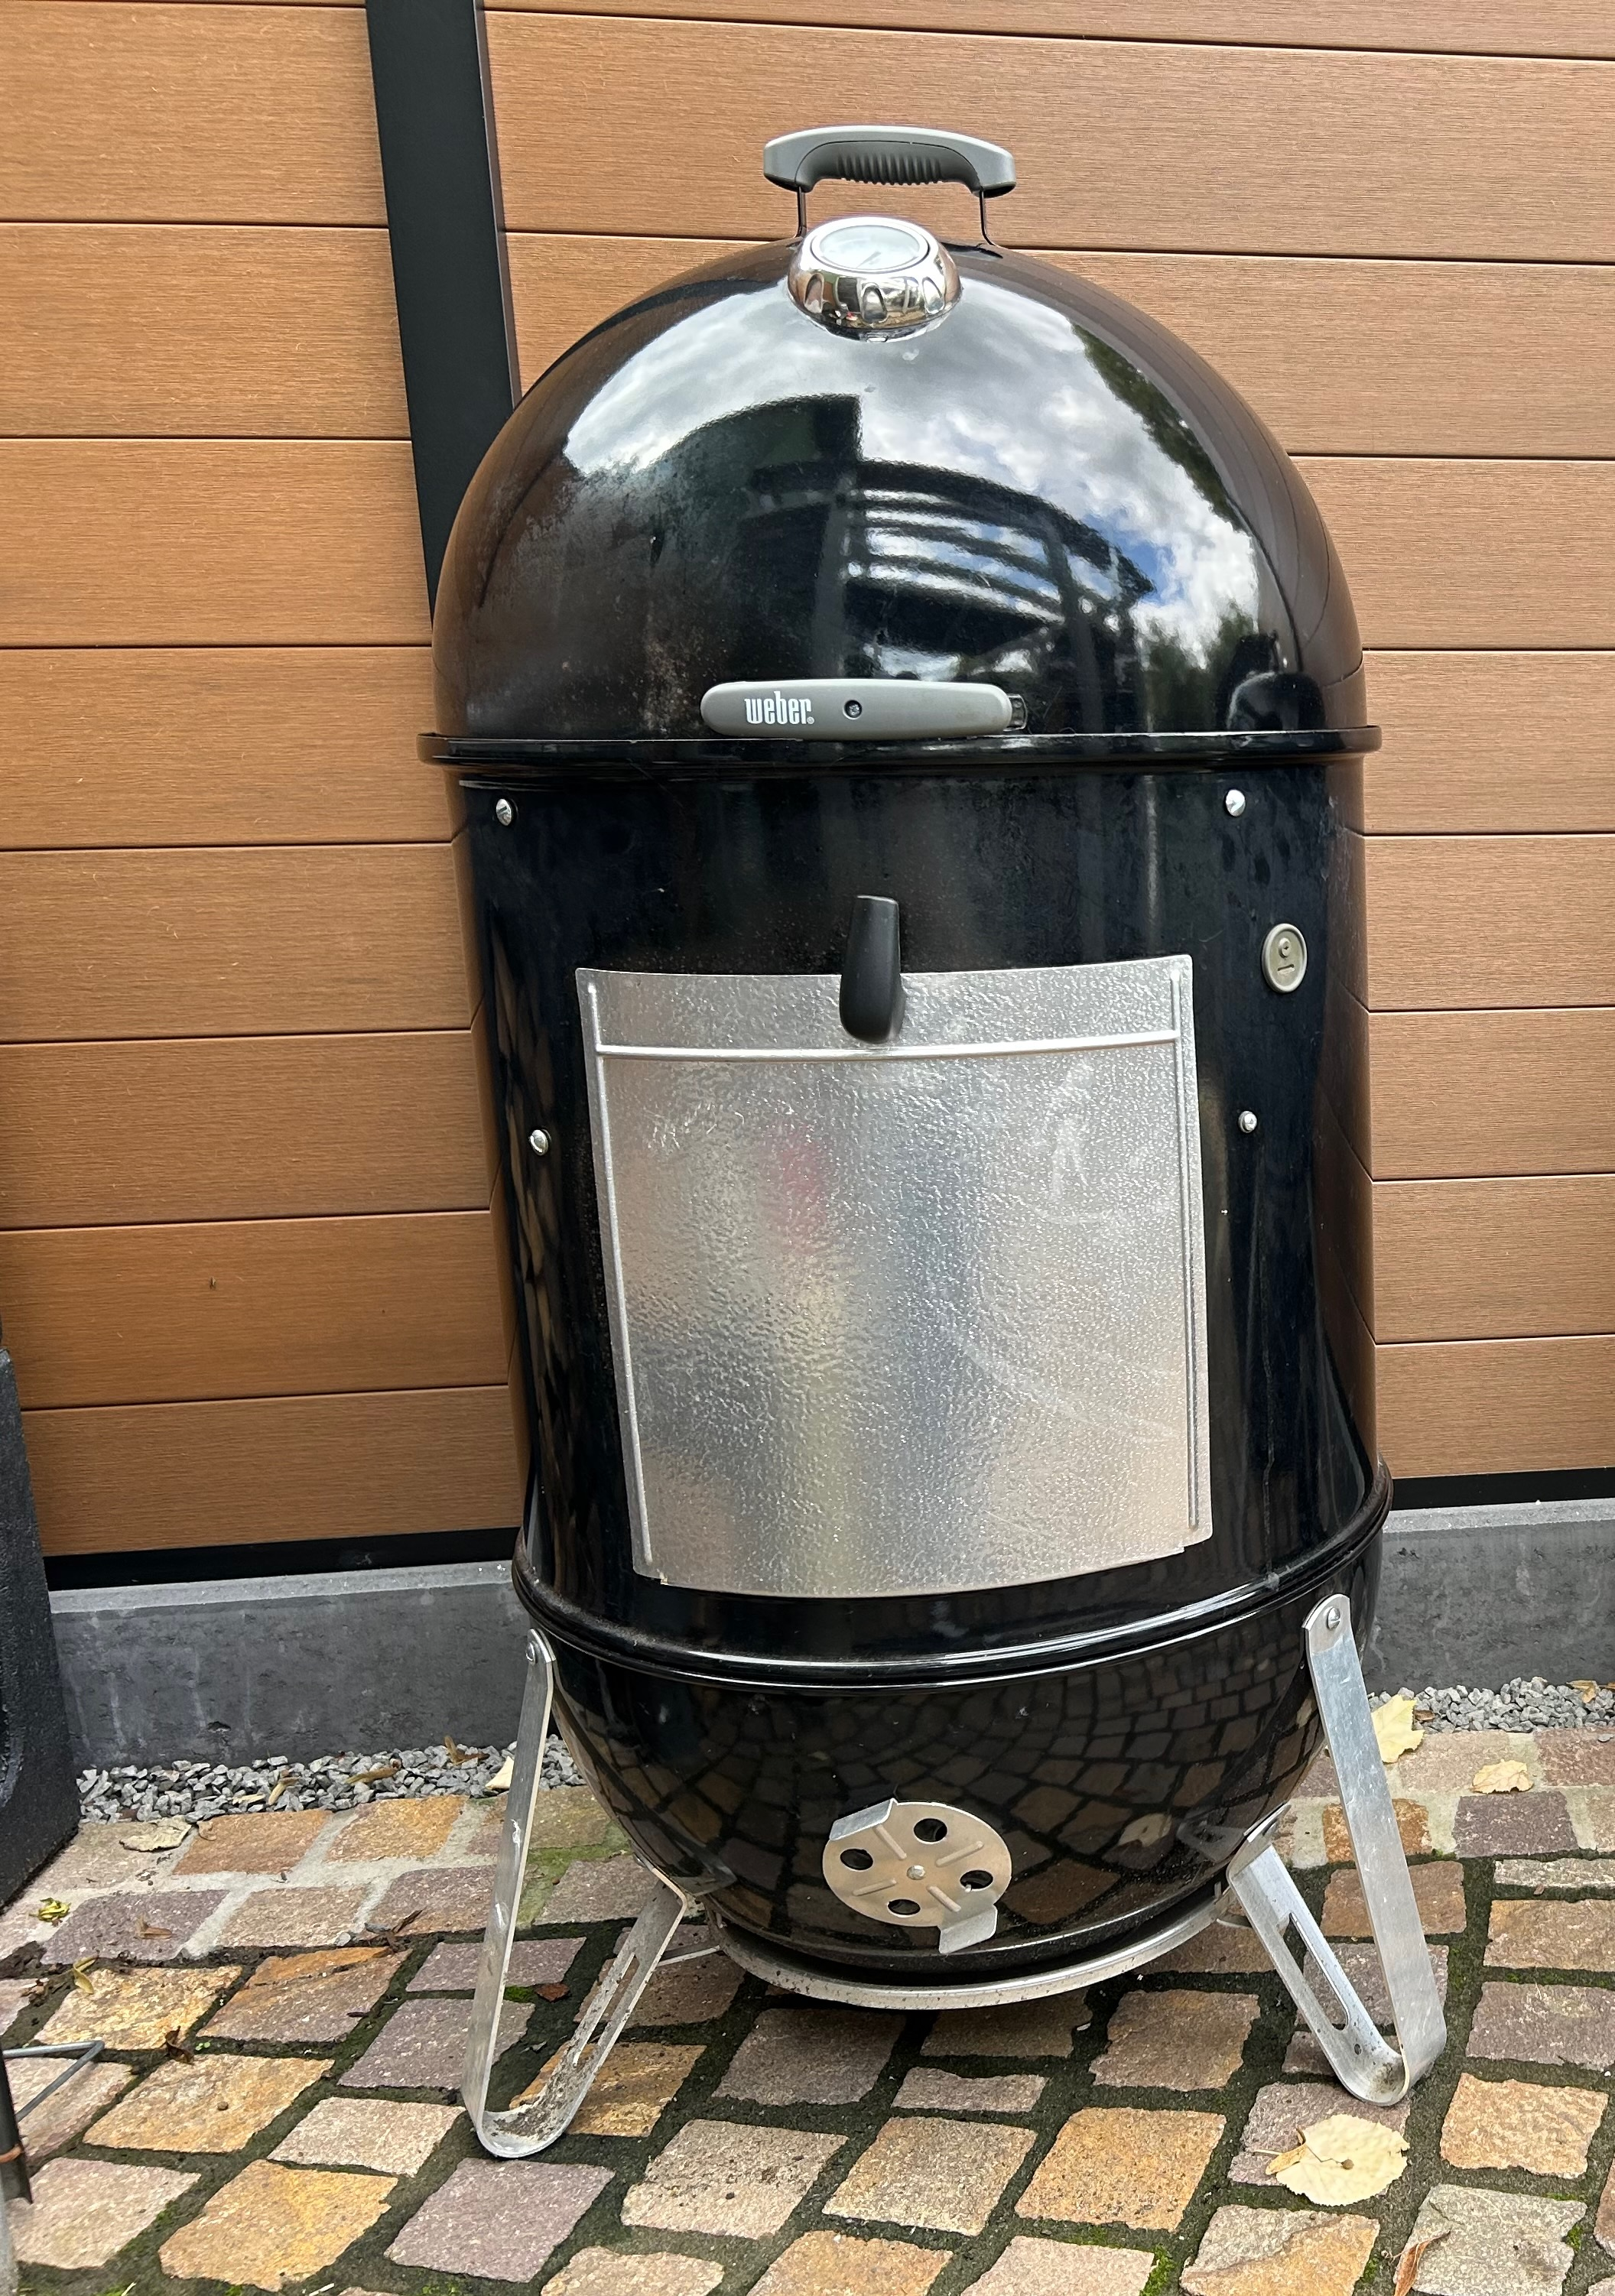
\includegraphics[width=.8\linewidth]{pics/Smoker}
			\captionof{figure}{Weber Water Smoker}
			\label{fig:Smoker}
		\end{minipage}%
	\end{figure}
	\newpage
	%Grills, Smoker
%!TEX root = Vorlage_Buch.tex

\chapter{Tierisch Gutes}\label{Chapter2}
\lettrine[lines=3]{I}{n diesem Kapitel} beschäftigen wir uns mit Fleisch, Fisch 
und Geflügel, das auf den Grill zubereitet wird.  
Genauso vielfältig wie die Grill-Geräte sind die Rezepte die auf den Grills 
zubereitet werden. Für jede Art von Grill gibt es 
Rezepte die dafür wie geschaffen sind.

\section{Rind}

Die große Auswahl an Fleischrinderrassen bietet letztendlich für jeden 
Geldbeutel und Geschmack das richtige Fleisch. 

\begin{description}
	\item[Aberdeen Angus] Weltweit verbreitet, schön mamoriertes, 
	aromatisches Fleisch
	\item[Brangus] Kombinationsrasse aus Brahman und Angus, beliebt in 
	Südamerika, Australien und Asien, schön mamoriertes, aromatisches 
	Fleisch
	\item[Charolais] ist ein französisches Rind, das wegen seinem 
	mageren, mit feinen Fettadern durchzogenem Fleisch bei Kennern sehr 
	beliebt ist
	\item[Chianina] Eine der ältesten und die größte Rinderrasse der Welt. 
	Das magere Fleisch schmeckt unvergleichlich zart und würzig.
	\item[Deutsch Angus] Ist für die Freilandhaltung gut geeignet. Das 
	Fleisch ist besonders schmackhaft durch die feinen Fleischfasern und 
	die gute Mamorierung.
	\item[Galloway] Ursprung südwestliches Schottland, kommt gut mit 
	Trockenheit, Kälte und Schnee zurecht. Das saftige, aromatische 
	Fleisch ist gut mamoriert und weist eine leichte Wildnote auf.
	\item [Das ursprünglich aus England stammende Hereford-Rind] passt 
	sich an jedes Klima an und ist somit weltweit vertreten. Das Fleisch 
	zeichnet sich durch intensiven Geschmack und eine feine Mamorierung 
	aus.
	\item [Das Heckrind] wurde in 1930er Jahren von den Gebrüdern Heck 
	gezüchtet. Sie kreuzten 8 Wildrassen und 17 Hausrassen mit dem Ziel, den 
	Auerochsen wieder aufleben zulassen, der im 17ten Jahrhundert 
	ausgestorben ist. Das Ziel wurde nicht erreicht, heraus kam allerdings ein 
	robustes, krankheitsresistentes Rind, das ganzjährig auf der Weide steht da 
	es sehr temperaturtolerant ist. Das Fleisch hat einen intensiven Geschmack 
	und ist durch die kurzen Fleischfasern sehr zart und reich an Vitaminen und 
	Omega-3-Fettsäuren.
	\item[Das Hinterwälder Rind] kommt aus dem Schwarzwald und ist fast 
	ausgestorben. Nur der Initiative einer weniger Landwirten ist der 
	Fortbestand zu verdanken. Das Fleisch ist sehr selten und zeichnet 
	sich durch eine feine Faser mit solider Fetteinlagerung aus. Durch die 
	natürliche Fütterung mit Gras und Heu prägt sich ein mineralisch 
	-intensiver Geschmack aus.
	\item[Kobe-Rinder] kommen aus der japanischen Präfektur Hyogo mit 
	dem Verwaltungssitz Kobe. Die Rasse nennt sich Tajima, im Westen 
	allerdings Wagyu. Das Fleisch der Kobe-Rinder ist extrem Fett, das 
	zeigt sich an der hellroten bis rosa-roten Farbe, der Fleischgeschmack 
	ist sehr mild. Das Fleisch hat allerdings einen schönen Schmelz.
	\item[Limousin-Rinder] stammen aus der gleichnamigen Region in 
	Frankreich. Durch die zarte Faserung und das optimale 
	Fleisch-Fett-Verhältnis ist das Fleisch saftig und sehr zart.
	\item [Pinzgauer Rinder] haben eine dunkle Fleischfarbe, eine sehr 
	feine Verteilung des Fetts im Fleisch und ein stark mineralisches 
	Aroma, da die Tiere fast ausschließlich aus Weidehaltung stammen.
	\item [Rubia Gallega oder auch Galicisches Blondvieh] ist eine alte 
	spanische Hausrinderrasse aus Galizien. Genießer schätzen vor allem 
	die dunkle Fleischfarbe, die ausgeprägte Fettmarmorierung und das 
	intensiv-kräftige Aroma.
	\item [Schottische Highlands] leben das ganze Jahr im Freien und 
	werden gerne zu Landschaftspflege eingesetzt. Das Fleisch ist 
	kurzfaserig und dadurch zart und saftig.
	\item[Shorthorns] sind kleine englische Rinder, die rasch 
	ausgewachsen sind und dann zur Verfettung neigen. Das heißt, die 
	Energie im Futter wird in Form von Fett in den Muskel eingelagert. Das 
	sorgt für einen zarten und saftigen Schmelz.
	\item[Simmentaler Rind] kommt aus dem gleichnamigen Simmental im 
	Berner Oberland. In Deutschland und Österreich gehören sie zu dem 
	bedeutendsten Rinderrassen. Gourmets schätzen den aromatischen 
	Geschmack und die feine Mamorierung.
	\item[Das Wagyu-Rind] hat die höchste Fettmamorierung aller 
	Rinderrasen, welche für die Saftigkeit und Zartheit diese Fleisches 
	verantwortlich ist. Siehe auch Kobe-Rind.
\end{description}

\subsection{Roastbeef vom Keramikgrill}
Roastbeef ist ein besonders zartes und saftiges Stück Fleisch, das aus 
dem hinteren Rücken des Rindes stammt. Es ist bekannt für seine feine 
Marmorierung und wird oft im Ganzen zubereitet. Traditionell wird es in 
Großbritannien als klassisches Sonntagsessen serviert. 

\paragraph{Geräte}

\begin{itemize}[noitemsep]
	\item Kamado Grill (Keramikgrill)
\end{itemize}


Vorbereitung des Kamado Grills: Der Feuerkorb wird abgeteilt und eine Hälfte
mit Holzkohlen gefüllt. Die Seite auf mit der 
Holzkohle für direkte Hitze
vorbereiten. Das heißt eine Hälfte des Grillrosts auf die unterste Stufe 
über die Holzkohle legen. Die andere Seite für indirekte Hitze vorbereiten. 
Einen halben Deflektorstein neben den Grillroast auf die unterste Stufe 
legen. Eine Hälfte der Fettauffangschale auf den Deflektorstein stellen 
und die zweite Rosthälfte auf die oberstes Stufe legen. Den Grill anheizen 
und die Temperatur auf 150℃ einstellen. Die Temperatur wird im Dom 
gemessen
und ist daher niedriger als direkt über den Kohlen. Diesen Umstand 
machen
wir uns zu Nutze, in dem wir das Roastbeef in der indirekten Zone auf den
gewünschten Gargrad ziehen. Bei einem Roastbeef ist meines Erachtens
eine Temperatur 55℃ bis 57℃ (medium rare bis medium) mit einer 
Tendenz
zu 57℃ anzustreben, da die meisten Menschen medium gegartes Fleisch
bevorzugen.

\paragraph{Zutaten}

\begin{itemize}[noitemsep]
	\item Roastbeef (ca. 1,5 kg)
	\item 10 g/ kg Fleisch grobes Himalaya-Salz
	\item 5 g bis 7 g schwarzer Pfeffer (hier Whisky-Pfeffer), ganze Körner 
	im Mörser zerkleinert
\end{itemize}

\paragraph{Zubereitung}

Salz und Pfeffer mischen. Das Roastbeef von allen Seiten gleichmäßig mit 
der Salz-Pfeffermischung würzen und diese leicht einmassieren. Danach
das Roastbeef auf der direkten Hitze von allen Seiten angrillen, bis die
Oberfläche karamellisiert und sich Röststoffe gebildet haben. Wenn das
Fleisch auf allen Seiten angeröstet ist, wird es auf die indirekte Hitze 
gelegt
und auf die gewünschte Temperatur hochgezogen. Das Fleisch bei 
erreichen
der Temperatur vom Grill nehmen und in Butterbrotpapier oder besser in
Butchers paper einwickeln und für 10 bis 20 Minuten in einer 
Warmhaltebox
ruhen lassen. Das Fleisch im dünne Scheiben schneiden und servieren, 
siehe Abbildung~\vref{fig:Roastbeef}
Dazu Beilagen nach Wahl reichen.

Alternativ kann das Roastbeef auf dem Kugelgrill zubereitet werden. Dazu
muss der Kugelgrill mit der Zwei-Zonen-Glut (siehe Kapitel~\ref{Chapter1} 
\vref{fig:ZweiZonen}) vorbereitet werden. Auf dem
Gasgrill wird die Temperatur mit einem oder zwei Brennern eingestellt und
das Fleisch auf der direkten Hitze angegrillt.
\newpage
\begin{figure}[htbp]
	\centering
	\begin{minipage}{1\textwidth}
		\centering
		\includegraphics[width=1\linewidth]{pics/Roastbeef_2}
		\captionof{figure}{Roastbeef vom Keramikgrill}
		\label{fig:Roastbeef}
	\end{minipage}
\end{figure}
\newpage

\subsection{Roastbeef unter der Kräuterkruste}

\paragraph{Geräte}

\begin{itemize}[noitemsep]
	\item Napoleon Gasgrill Rogue 425
\end{itemize}

\paragraph{Zutaten}

Für das Roastbeef:

\begin{itemize}[noitemsep]
	\item Roastbeef (ca. 1,5 kg) 
	\item 100 g Semmelbrösel
	\item 100 g weiche Butter
	\item 2 TL körniger Senf
	\item 2 EL Olivenöl
	\item Salz  \& Pfeffer
	\item 2 Zweige Rosmarin
	\item 2 Knoblauchzehen
\end{itemize}

Für die Soße:

\begin{itemize}[noitemsep]
\item 1 Karotte
\item 1 Zwiebel
\item 50 g Lauch
\item 1 Knoblauchzehe
\item 1 EL Tomatenmark
\item 1 TL Paprikapulver
\item 1 TL Mehl
\item 300 ml Schwarzbier (bei Köstritzer Schwarzbier)
\item 300 ml Rinderfond
\end{itemize}
\newpage

\paragraph{Zubereitung}

Die Zubereitung des Roastbeefs erfolgt im Gasgrill. Alternativ kann das
Gericht auch im Backofen zubereitet werden. 

Den Gasgrill auf ca. 230℃ 
bis 260℃ aufheizen und das Roastbeef von allen Seiten scharf anbraten. Das 
Fleisch zur Seite legen damit es Temperatur verliert, so lässt die Kräuterkruste 
besser aufbringen, da die Butter bei zu hoher Temperatur schnell schmilzt.

Während das Fleisch und der Grill abkühlen, widmen wir uns der Kräuterkruste. 
Dafür werden alle Zutaten in einer Schüssel vermengt und 
verrührt.
Wenn alles ordentlich vermengt ist, wird die Kruste gleichmäßig auf das
Fleisch verteilt.

Bevor das Fleisch jetzt zum Garen auf den Grill gestellt wird, muss
die Soße zubereitet werden. Eine Gusseiserne Pfanne auf dem 
Seitenkochfeld
des Gasgrills erhitzen und das Gemüse in der Pfanne angebraten. Wenn 
das
Gemüse angebraten ist und die Zwiebeln glasig sind, kommen Mehl,
Paprikapulver und das Tomatenmark dazu und werden kurz mit 
angebraten.
Anschließend wird alles mit dem Schwarzbier abgelöscht und mit dem
Rinderfond aufgefüllt und 2 bis 3 Minuten gekocht.

Jetzt wird das Fleisch mit der vorher aufgetragenen Kruste nach oben in
die Soße gelegt, ein Kerntemperaturfühler in das Fleisch eingesteckt und in den 
vorgeheizten Grill gestellt.
Kurz bevor das Fleisch die gewünschte Kerntemperatur (ich empfehle 55°C bis 
57°C) erreicht hat, wird
der Heckbrenner des Grills angestellt und auf die höchste Stufe 
eingestellt, damit die Kruste kross wird und eine schöne Farbe bekommt. 
Aufpassen!
Das geht sehr schnell.

\begin{figure}[htbp]
	\centering
	\begin{minipage}{1\textwidth}
		\centering
		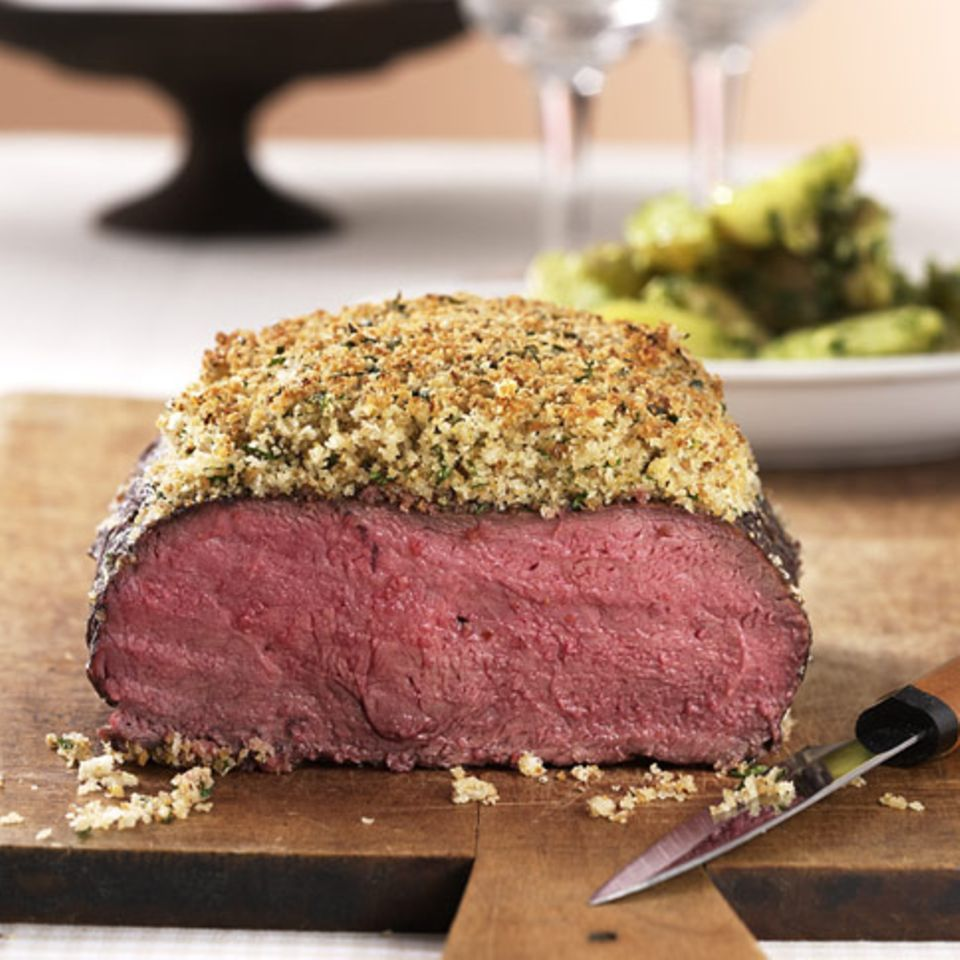
\includegraphics[width=1\linewidth]{pics/roastbeefmitkraeuterkruste}
		\captionof{figure}{Roastbeef vom Keramikgrill}
		\label{fig:Roastbeef}
	\end{minipage}
\end{figure}
\newpage

%\begin{figure}[htbp]
%	\centering
%	\begin{minipage}{1\textwidth}
%		\centering
%		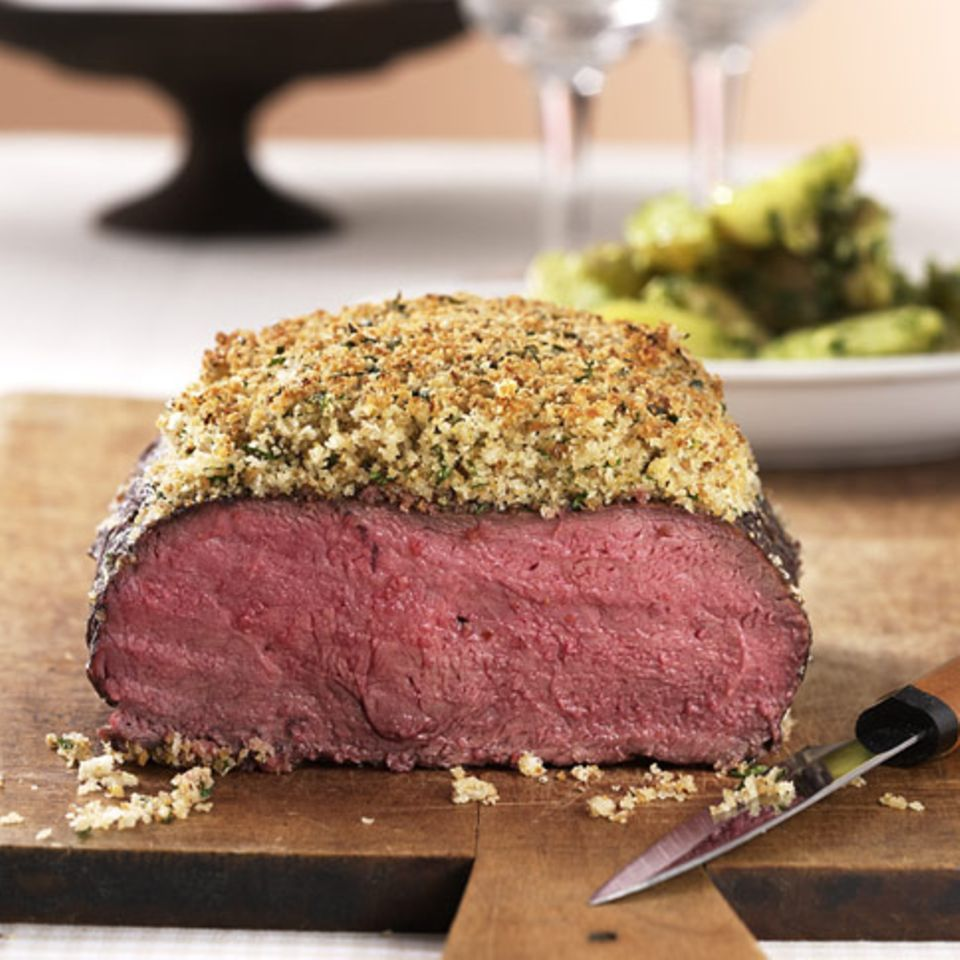
\includegraphics[width=1\linewidth]{pics/roastbeefmitkraeuterkruste}
%		\captionof{figure}{Roastbeef mit Kräuterkruste vom Gasgrill}
%		\label{fig:Roastbeef}
%	\end{minipage}
%\end{figure}
%\newpage

\subsection{Beef brisket}

\paragraph{Geräte}

\begin{itemize}[noitemsep]
	\item Water smoker
\end{itemize}

\paragraph{Zutaten}

\begin{itemize}[noitemsep]
	\item 1 Rinderbrust full packer von der Simmentaler Färse(Brust bestehend aus Flat and point, pariert ca. 5,5 bis 6,0 kg)
	\item grobes Salz (hier Himalaya-Salz, ca. 9 g/ kg Fleisch)
	\item schwarzer Pfeffer, ganz (ich verwende Telly Cherry Pfeffer, ca. 9 g/ kg Fleisch)
	\item Rauch (ich verwende Apple Wood Chuncks)	
\end{itemize}

\paragraph{Zubereitung}

Den Water Smoker vorbereiten und eine Temperatur von 135°C bis 140°C anvisieren.
Die Rinderbrust parieren, d. h. überflüssiges Fett entfernen, die Kanten rund schneiden, 
lose Enden sollten entfernt werden. Das Brisket mit dem Rub großzügig und gleichmäßig 
einreiben, wer mag kann noch etwas Zwiebel- und Knoblauchpulver zu der 
Salz-Pfeffermischung geben. Das Fleisch auf den oberen Rost legen und den Deckel 
wieder schließen. Apple Wood Chuncks auf die Holzkohle legen, so dass Rauch für ca. 1 
Stunde entsteht. Das Fleisch von Zeit zu Zeit mit etwas Flüssigkeit besprühen, damit die 
dünnen Enden nicht zu stark bräunen. Sobald das Fleisch eine gute Farbe hat, nach ca. 
2,5 bis 3 Stunden, in Butchers paper mit etwas Rinderfond, Apfelsaft oder Wasser lagen 
und solange weitergaren bis ein e Kerntemperatur von 95°C erreicht wird. Wichtiger als 
die Temperatur ist allerdings das widerstandslos eindrigen des Messfühlers. Sobald 
noch eine spürbarer Widerstand zu fühlen ist, ist das Brisket noch nicht fertig. 

Wenn das Brisket fertig gegart ist, noch eingepackt in eine Thermobox oder Styroporbox 
legen und eine halbe bis eine Stunde ruhen lassen. Danach das Brisket (siehe siehe Abbildung~\vref{fig:Brisket})mit Coleslaw
 (Rezept siehe Kapitel~\ref{Chapter5} \vref{Coleslaw}) und beliebigen Beilagen servieren.

\begin{figure}[htbp]
	\centering
	\begin{minipage}{1\textwidth}
		\centering
		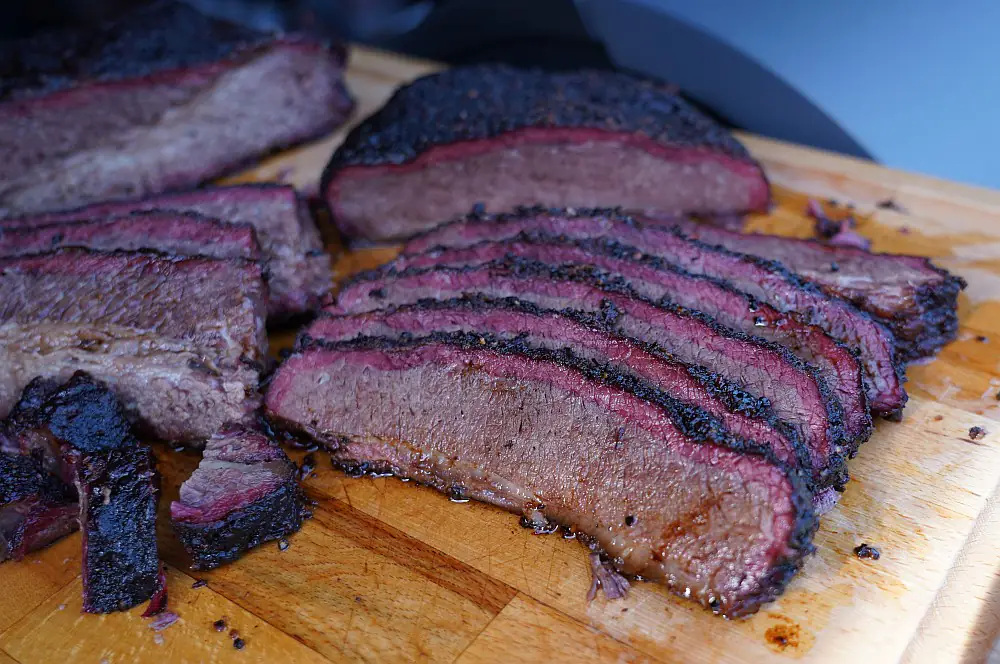
\includegraphics[width=.9\linewidth]{pics/Brisket}
		\captionof{figure}{Beef Brisket vom Water Smoker}
		\label{fig:Brisket}
	\end{minipage}
\end{figure}
\newpage

\subsection{Tomahawk Steak}

\paragraph{Geräte}

\begin{itemize}[noitemsep]
	\item Oberflächengrill Beefbox
	\item Keramikgrill
\end{itemize}

\paragraph{Zutaten für 2 Personen}

\begin{itemize}[noitemsep]
	\item 1 Tomahawk Steak (ca. 1,1 kg zur Metzgers Freude kann es auch ein 
	wenig mehr sein)
	\item Salz (ich benutze Himalaya-Salz aus der Mühle)
\end{itemize}

\paragraph{Zubereitung}

Den Keramikgrill hochheizen und die Temperatur auf 150°C einstellen.
Das Steak in der Beefbox von jeder Seite ca. 1 Minute und 30 Sekunden scharf 
angrillen, evtl. kann es länger gehen bis das Fleisch schön karamellisiert ist.
Das angegrillte Steak auf dem Keramikgrill je nach Geschmack garziehen siehe 
Abbildung~\vref{fig:Toma2}. Auf einem Holzbrett anrichten in Tranchen 
schneiden und servieren.
Dazu den Eisbergsalat mit Champignons und Tomatendressing reichen.
Ich bevorzuge dazu einen schönen Shiraz, z.B. Fat Baron 2022.
\newpage
\begin{figure}[htbp]
	\centering
	\begin{minipage}{1\textwidth}
	\centering	
	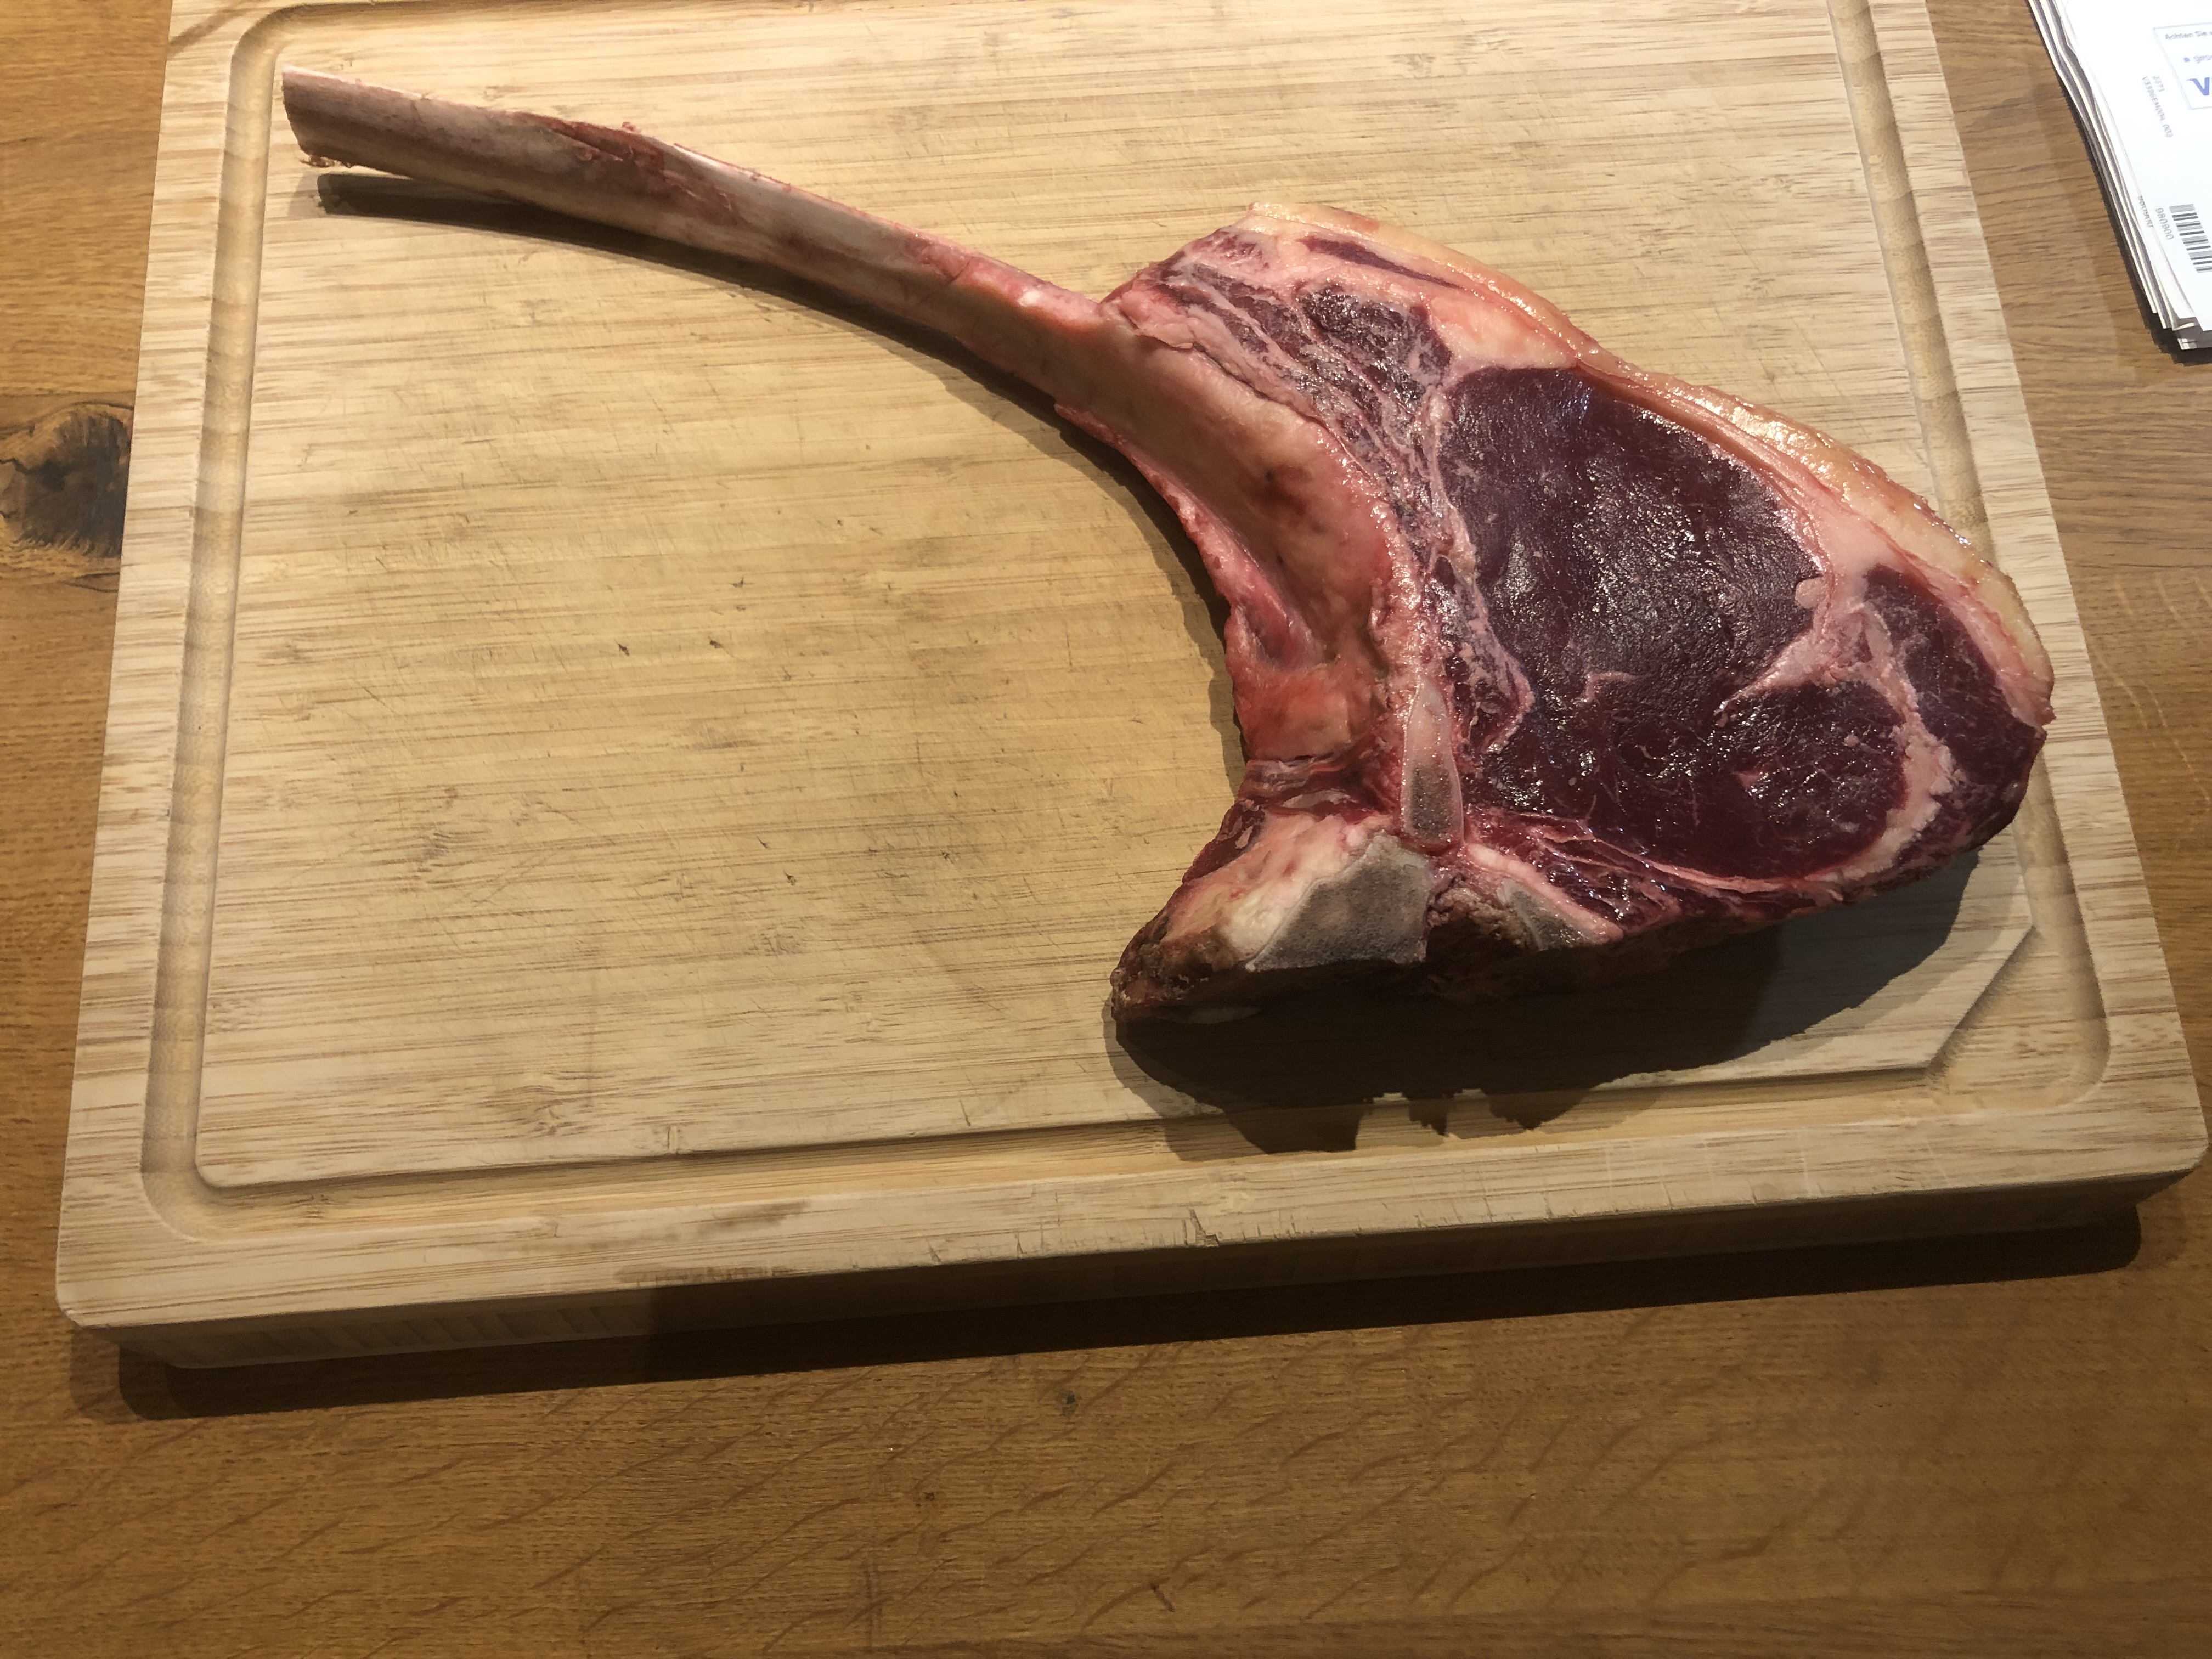
\includegraphics[width=1\linewidth]{pics/Tomahawk_roh}
	\captionof{figure}{Tomahawk Steak vor dem Grillen}
	\label{fig:Toma1}
	\end{minipage}
\end{figure}

\begin{figure}[htbp]
	\centering
	\begin{minipage}{1\textwidth}
	\centering
	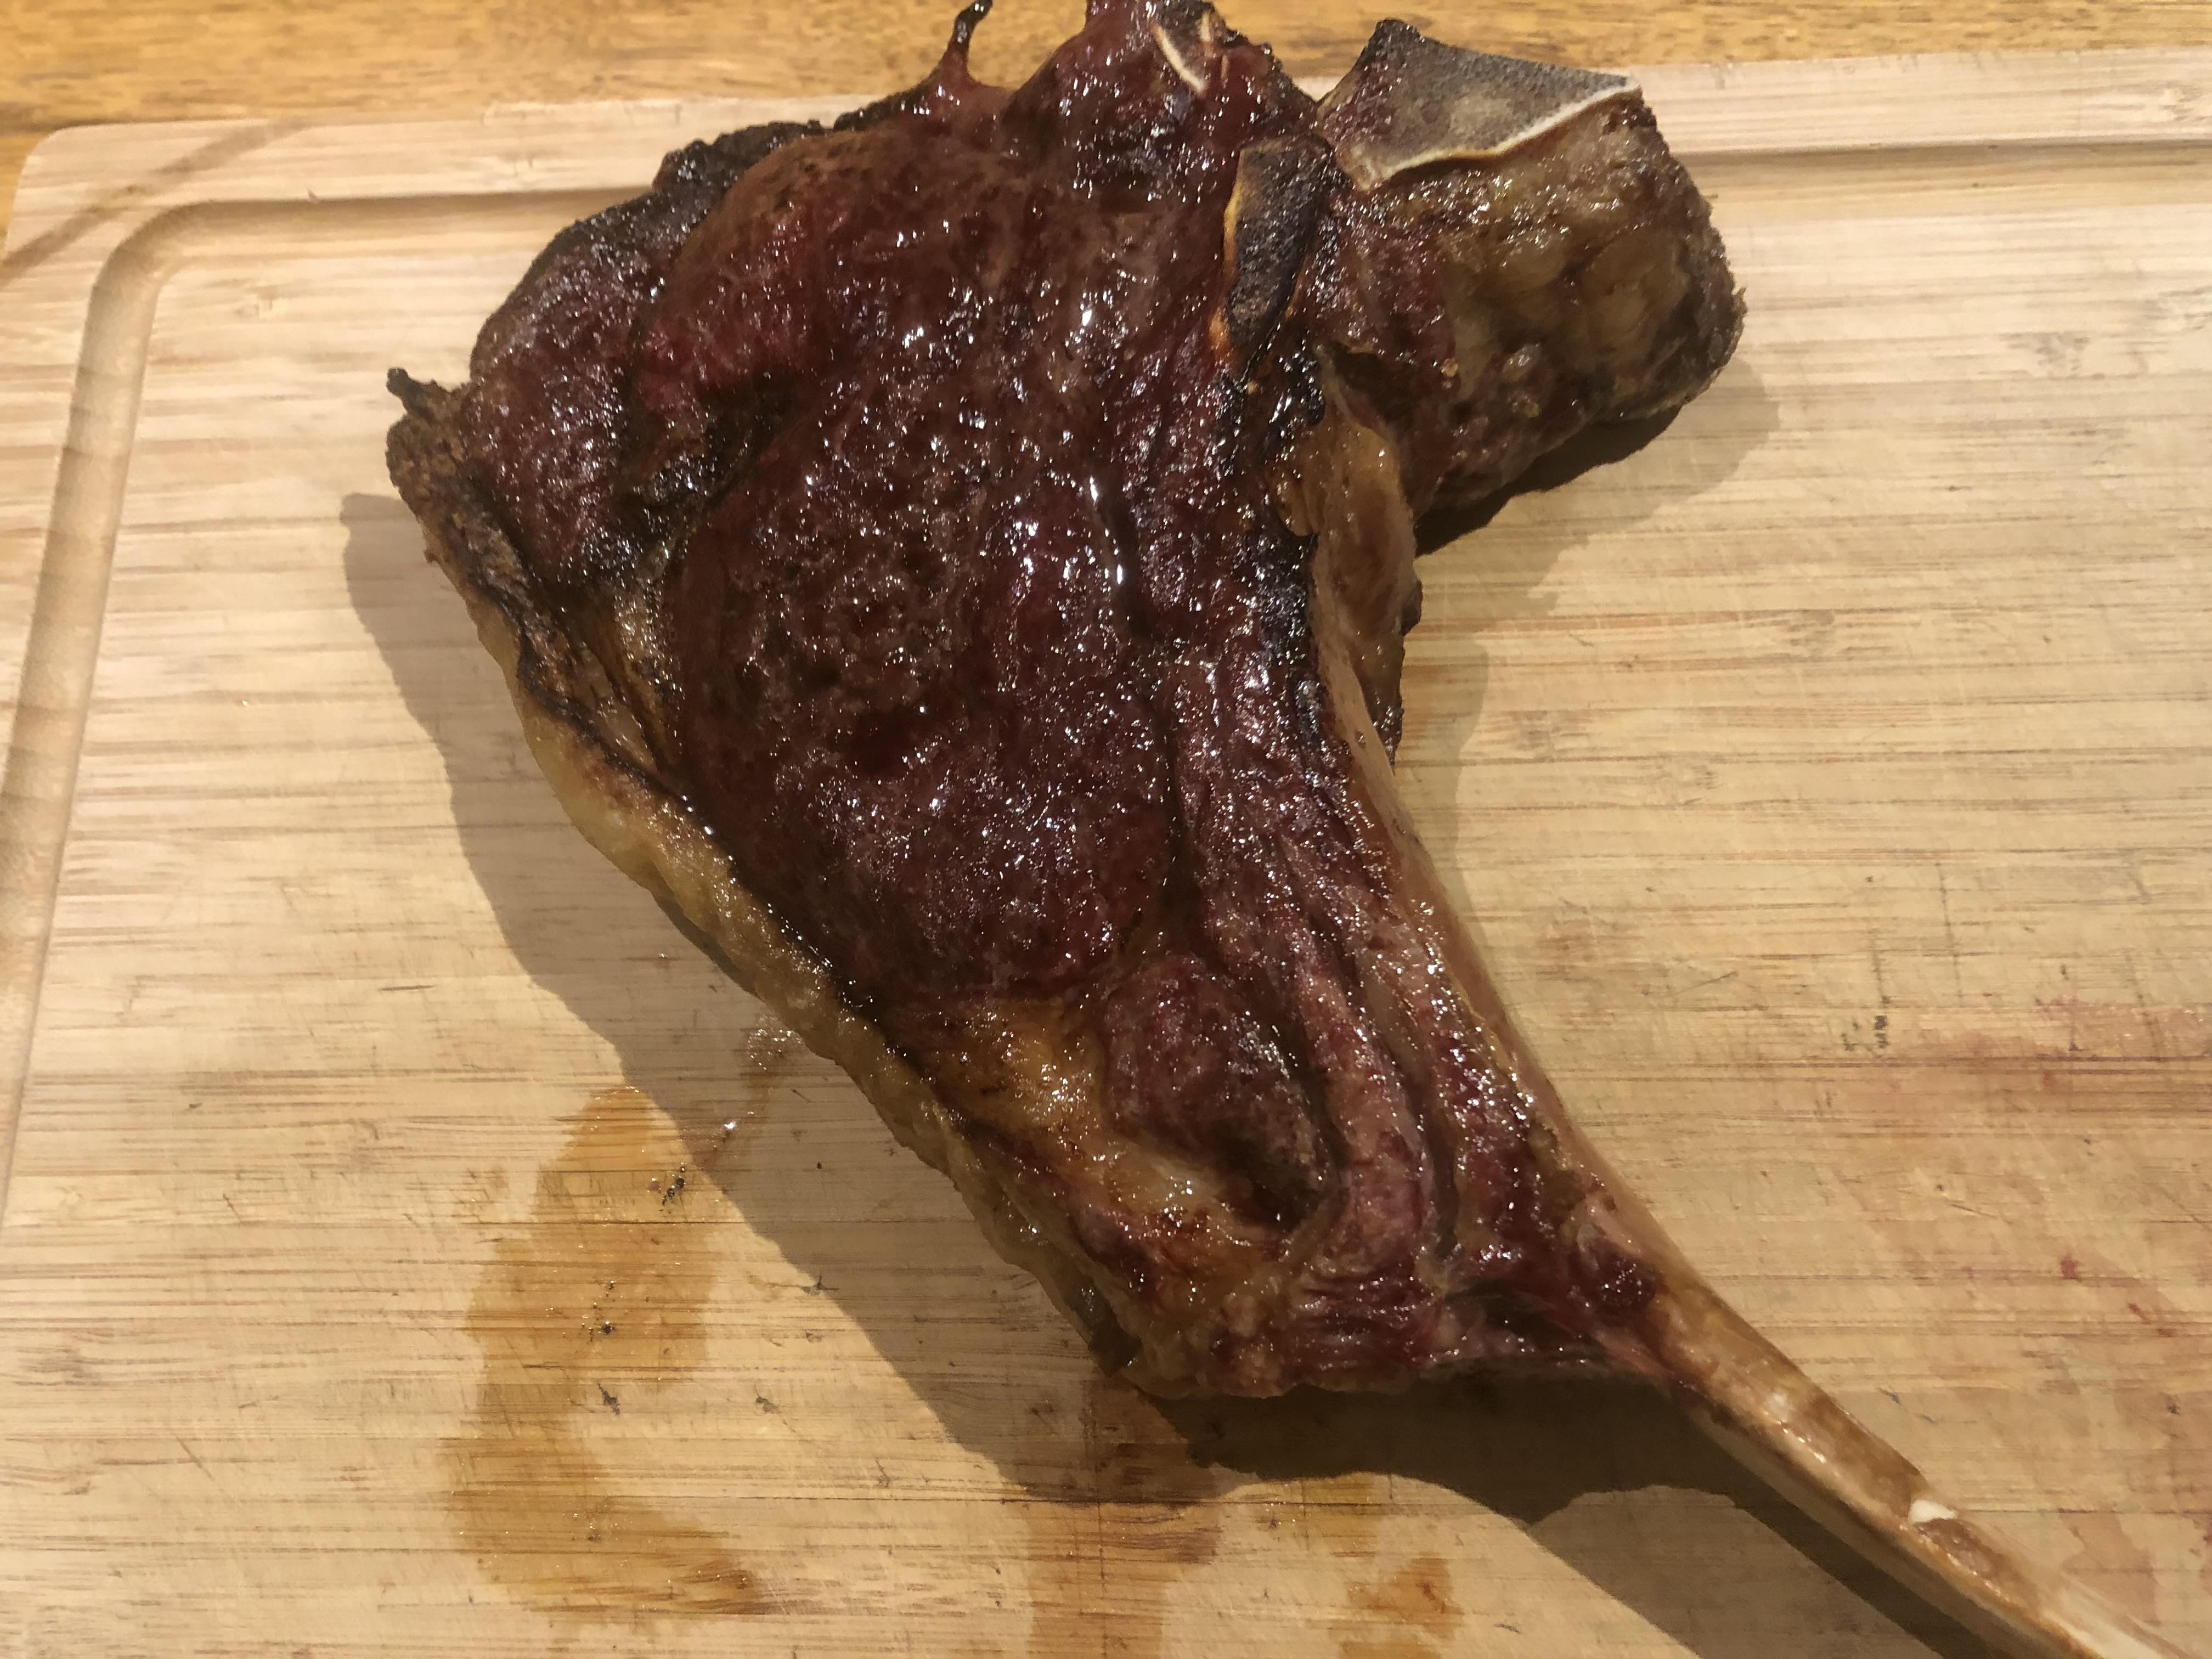
\includegraphics[width=.9\linewidth]{pics/Tomahawk_gegrillt}
	\captionof{figure}{Tomahawk Steak}
	\label{fig:Toma2}
	\end{minipage}
\end{figure}
\newpage

\subsection{Chili con carne}
Die Staaten Texas, New Mexico und Arizona erheben Anspruch auf den Ursprung des Chili con carne. Es gibt viele Geschichten über das Urrezept. Unbestritten ist jedoch 
der mexikanische Einfluss, in der mexikanischen Küche werden verschiedene 
Chilisorten eingesetzt um den Geschmack zu variieren.

Hier werde ich zwei Rezepte vorstellen, ein schwarzes, schweres Chili das 
eher in die Wintermonate passt und ein leichtes helles Chili Rezept 
siehe~\vref{Helles Chili}, das perfekt für die Sommermonate ist.

\subsubsection{Schwarzes Chili}
Dieses schwarze Chili ist sehr schwer und mit seinem Gewürzen eher für die 
kalten Herbst- und Wintermonate geeignet. Die schärfe des Chilis ist wie ein 
innerer Ofen und sorgt für eine angenehme Wärme.

\paragraph{Geräte}

\begin{itemize}[noitemsep]
	\item Dutch oven
\end{itemize}

\paragraph{Zutaten Chili}

\begin{itemize}[noitemsep]
	\item 1 große Zwiebel(n), rot
	\item 2 Knoblauchzehe(n)
	\item 500 g Hackfleisch, vom Rind
	\item 1 Dose/n Tomate(n) (400 g)
	\item 2 Dose/n Bohnen, schwarz (400 g)
	\item 2 cl Whisky (Bei mir 10 Jahre alter Laphroig von der Isle of Islay, einer 
	der rauchigsten Whiskys der Welt)
	\item 200 ml Bier (Bei mir Köstritzer Schwarzbier)
	\item 100 ml Kaffee (Bei mir 2 Espressi à 50 ml)
	\item 1 EL	Tomatenmark
	\item Gewürzmischung, siehe Rezept in~\vref{Gewürzmischung}
	\item Salz \& Pfeffer
	\item Öl
	\item Butter
\end{itemize}



\paragraph{Zubereitung}

Rote Zwiebeln hacken. Knoblauchzehen mit einer Prise Salz zerdrücken. 
Hackfleisch in Öl anbraten. Wenn es durch ist, die gehackten Zwiebeln und 
zerdrückten 
Knoblauchzehen hinzufügen. Mit 1 EL Butter weiter braten, bis alles anröstet 
(nicht zu dunkel werden lassen). Mit Whisky ablöschen. Wenn der Whisky fast 
verkocht 
ist, die übrigen Zutaten bis auf die Bohnen hinzugeben. Mindestens 30 min 
weiter köcheln lassen - gern länger. Die Bohnen und Gewürze hinzugeben und 
mindestens
15 min weiter köcheln lassen. Abschmecken.

Am besten mit Maisbrot oder Baguette servieren.

Das Chili sieht richtig dunkel aus - fast schwarz (siehe 
Abbildung~\vref{fig:Schwarzes_Chili}) und riecht schon bei der Zubereitung 
lecker und lässt mir immer das Wasser im Munde zusammen laufen. Das Chili 
schmeckt intensiv, herb, leicht rauchig (dank Laphroig) und haut ordentlich 
rein. Das Chili ist für Erwachsene und nix für schlechte Nerven.
\newpage

\begin{figure}[htbp]
	\centering
	\begin{minipage}{1\textwidth}
		\centering
		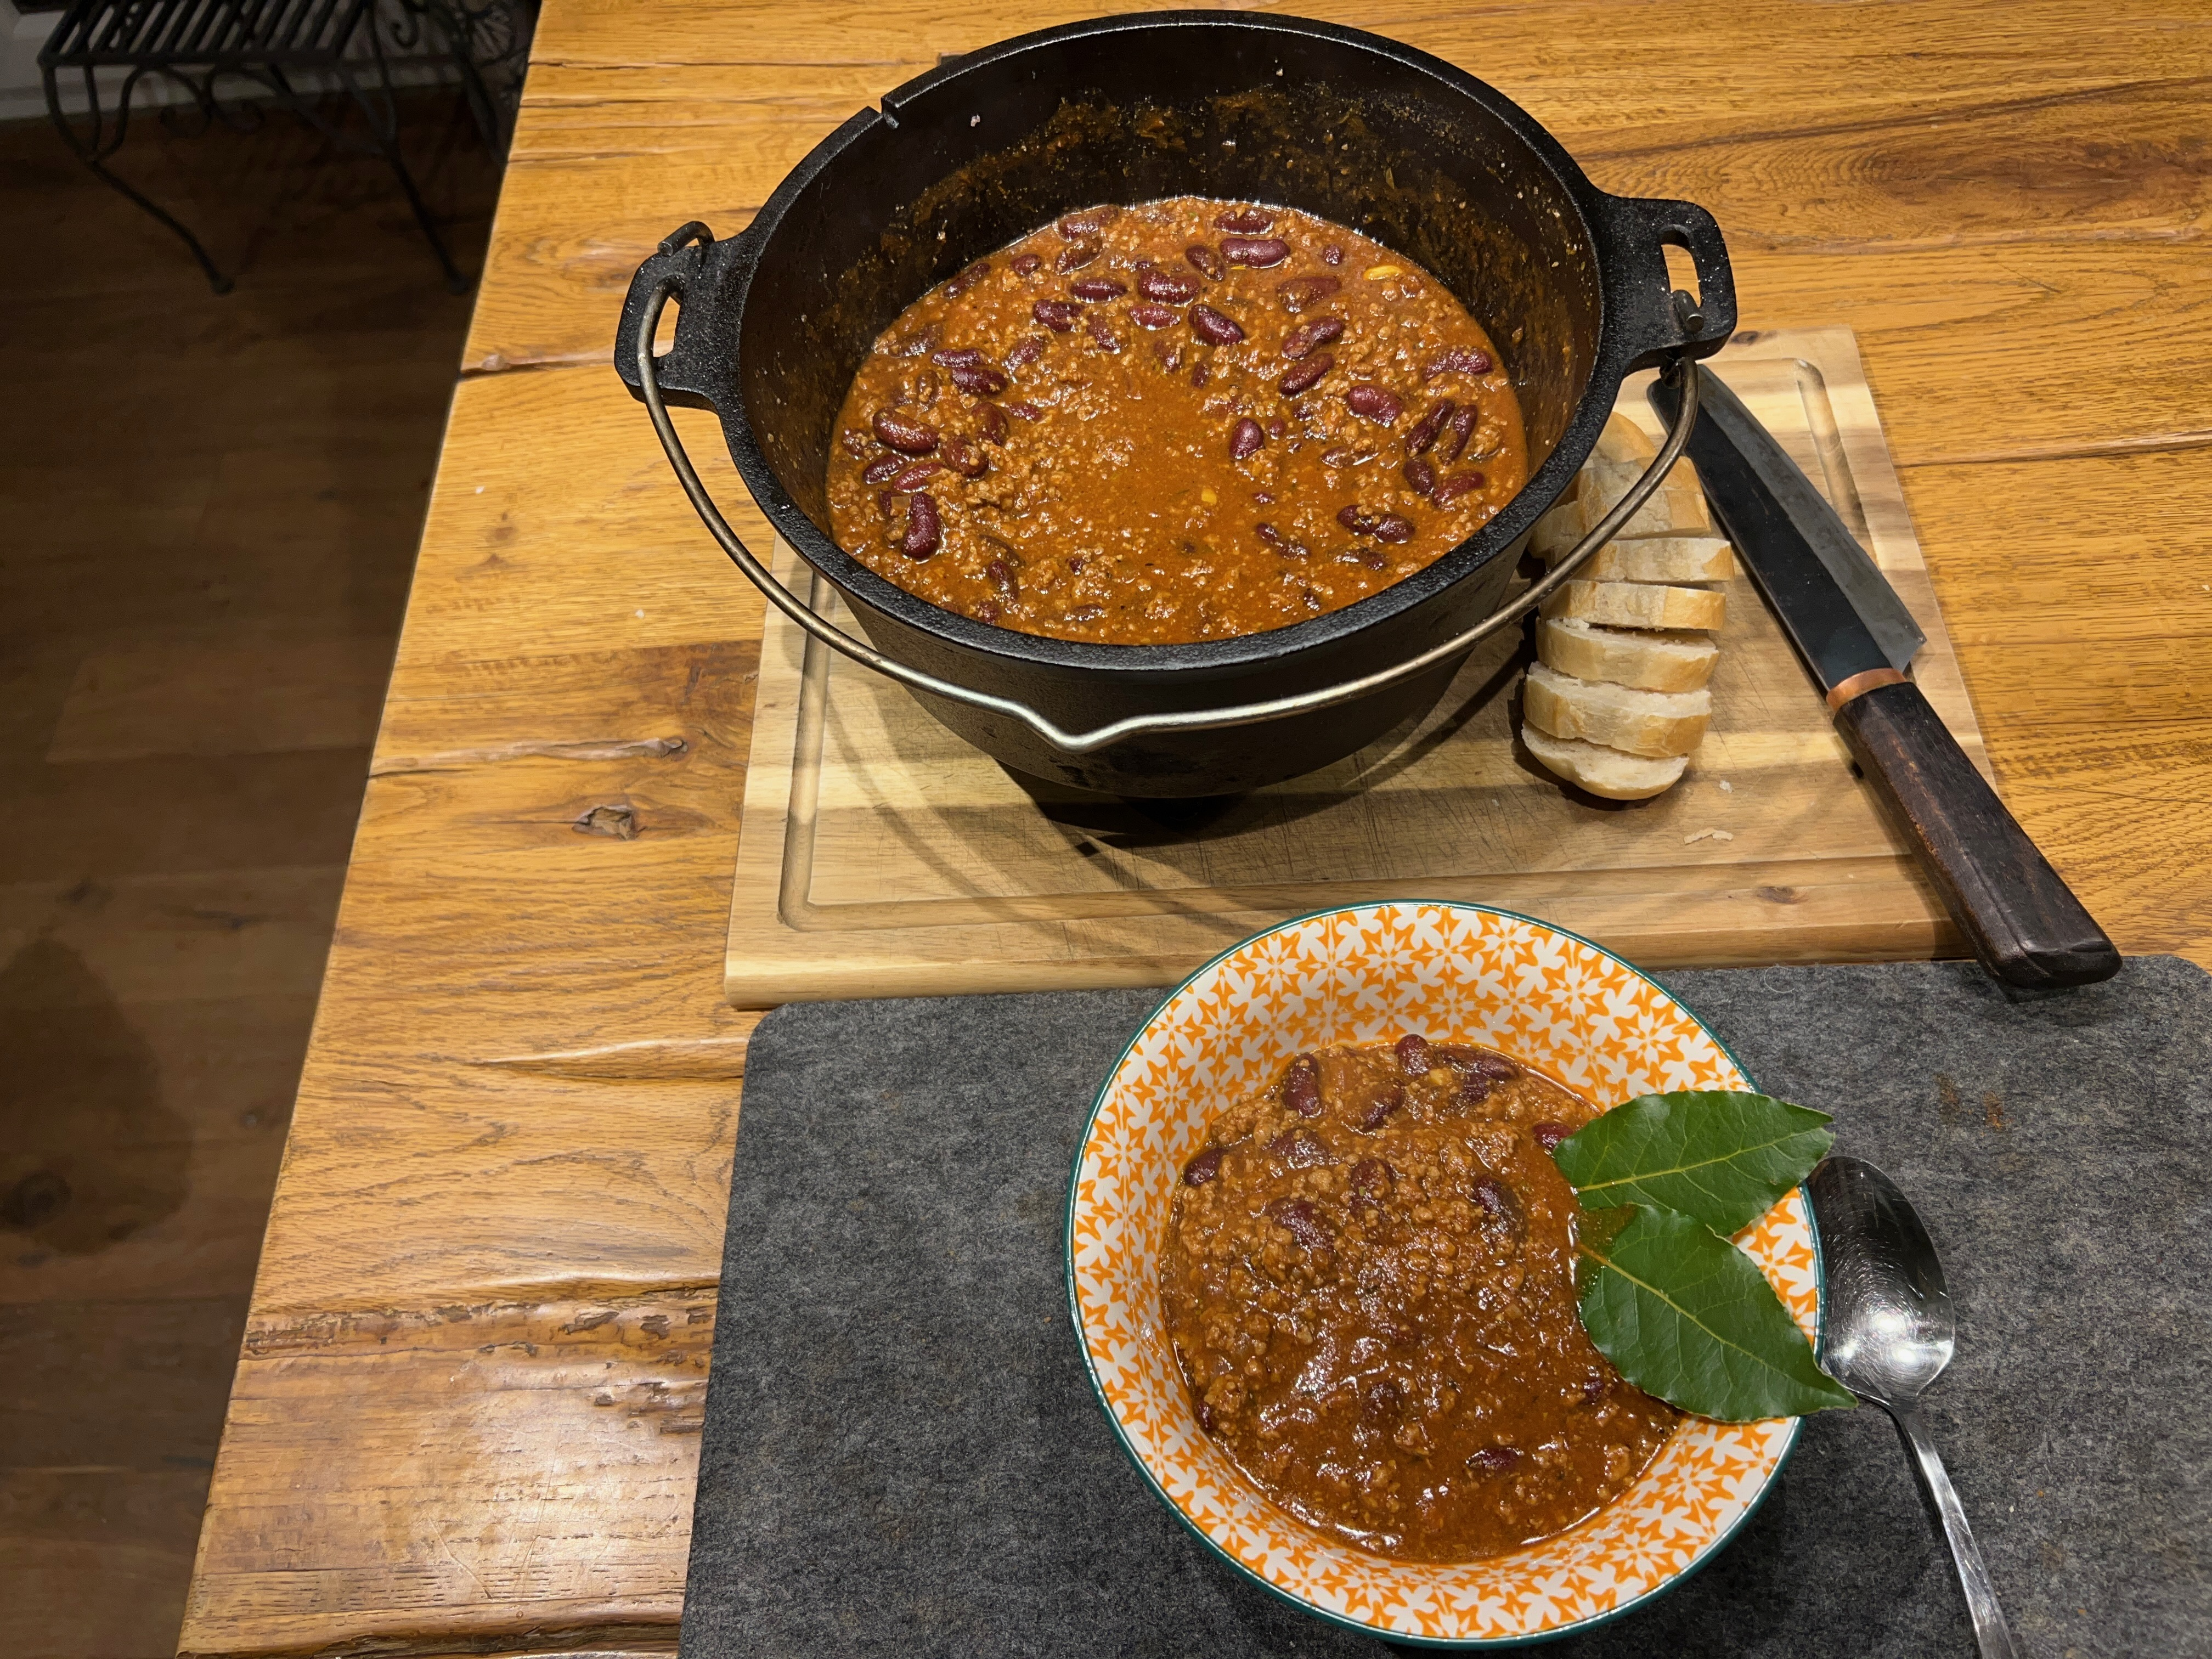
\includegraphics[width=.9\linewidth]{pics/Schwarzes Chili}
		\captionof{figure}{Schwarzes Chili aus dem Dutch oven}
		\label{fig:Schwarzes_Chili}
	\end{minipage}
\end{figure}
\newpage

\section{Schwein}

Es gibt deutlich weniger Schweinerassen die zum Grillen sehr beleibt 
sind. Hier werde ich einige der bedeutendsten Rassen vorstellen. Die 
Schweinerassen  sind sowohl in Gourmet-Kreisen als auch in der 
BBQ-Szene bekannt und beliebt.

\begin{description}
	\item[Das Bunte Bentheimer Schwein] stammt aus der Grafschaft 
	Bentheim im Emsland. Die Rasse wird wieder verstärkt gezüchtet und 
	somit wird die seltene Rasse weiträumiger Verfügbar. Das Fleisch hat 
	eine vergleichbar hohen Fettgehalt, das dadurch sehr schmackhafte 
	Fleisch ist in der gehobenen Gastronomie sehr gefragt.
	\item[Das Duroc] ist durch seine rot-braune Farbe und Schlappohren 
	leicht zu erkennen. Der Ursprung dieser Rasse ist nicht eindeutig 
	geklärt, zu kam sie entweder aus Südamerika mit den Spaniern oder 
	aus Afrika mit dem Umweg über Amerika. Das dunklere reine 
	Duroc-Fleisch enthält mehr intramuskuläres Fett und das schmeckt 
	Ihr auf eurem Teller: Das Fleisch ist feinfaserig, zart und hat einen 
	kräftigen Geschmack
	\item[Das Iberico-Schwein] ist wohl das edelste Schwein, es sind 
	halbwilde Schweine die pfleglos im freien gehalten werden. Da nicht 
	zugefüttert wird, ernähren sich die Schweine von Eicheln der Stein- 
	und Korkeichen sowie Kräutern. Als Eiweißquellen dienen, 
	Regenwürmer, Käfer, Schnecken. 
	\begin{itemize}[noitemsep]
		\item Jamón Ibérico de Bellota oder Jamón Ibérico terminado en 
		montanera stammt von freilaufenden Schweinen, die ca. 40\% ihres 
		Lebendgewichts durch Eicheln der Steineichen und Korkeichen 
		sowie Kräuter erreicht haben. Die Eicheln sorgen für den nussartigen 
		Geschmack.
		\item Jamón Ibérico de Recebo stammt von Schweinen, denen Eicheln 
		zugefüttert wurden. In dieser Zeit erhöht sich das Anfangsgewicht 
		durch Eicheln und Kräuter um ca. 30\%. Die Endmast erfolgt mit 
		Getreide und Viehfutter.
		\item Der Jamón Ibérico de Pienso (Campo) stammt von Schweinen, 
		die im Stall nur mit Getreide und Viehfutter gemästet wurden.
	\end{itemize}
\end{description}




\subsection{Spare ribs 3-2-1 Methode}
Spare ribs sind ein Bestandteil der "<Holly trinity of BBQ">  oder der 
">Dreifaltigkeit des BBQ">. Die beiden anderen Bestandteile sind Pulled 
Pork und Beef Brisket. 
Es gibt verschiedene Methoden Spare ribs zuzubereiten. Die wohl 
populärste ist die 3-2-1-Methode. Der Name erschließt sich aus der 
Zubereitung. Drei Stunden räuchern, 2 zwei Stunden dämpfen und eine 
Stunde glasieren. Abgeleitet davon gibt es noch die  4-1-1-Methode und 
die 5-0-1-Methode. Wie bei der 3-2-1-Methode bedeutet die erste Ziffer 
die Zeit in Stunden des Räucherns, die zweite Ziffer die Zeit in Stunden 
des Dämpfens und last but not least die dritte Ziffer die des Glasieren 
ebenfalls in Stunden.  
Bei der 3-2-1 werden die ribs so mürbe, dass sie fast vom Knochen fallen, 
im Jargon heißt es "> Falling of the bones"<. Bei der 4-1-1 Methode löst 
sich da Fleisch leicht vom Knochen hat aber noch Biss, während die 5-0-1 
Methode den meisten Rauchgeschmack mitbringt und deutlich bissfester 
ist als die anderen Methoden.

Als weitere Methoden sind

\begin{itemize}[noitemsep]
	\item Vorgaren im Backofen, scharf Angrillen und Glasieren
	\item Sous vide Garen, scharf Angrillen und Glasieren
	\item Schmoren im Dutch oven, scharf Angrillen und Glasieren
\end{itemize}
zu nennen.
\newline

\paragraph{Geräte}

\begin{itemize}[noitemsep]
	\item Kugelgrill
	\item Water Smoker
 	\item Gasgrill (min. 3 Brenner)
	\item Kamado Grill (Keramik Grill)
\end{itemize}

Die Handhabung der Geräte wird in Kapitel\ref{Chapter1} erklärt

\paragraph{Zutaten für 4 Personen}

\begin{itemize}[noitemsep]
	\item 2,0 bis 2,4 kg Spare ribs St. Louis Cut oder Baby Back Ribs
	\item Kansas City Rib Rub (Rezept siehe Kapitel~\ref{Chapter6} 
	\vref{Kansas})
\end{itemize}

Zutaten für die Glasur:
\begin{itemize}[noitemsep]
	\item 200 g Himbeermarmelade
	\item 100 ml Apfelsaft
	\item 1 EL Balsamico Essig
	\item Salz
	\item Pfeffer	
\end{itemize}

Vorbereitung: Bei dem Kugelgrill und dem Water Smoker Junks auf die Holzkohle geben. Hier Hickory oder Apfel.
Bei dem Kamado Grill Räucherchips verwenden, die uneingeweicht auf die Holzkohle gegeben werden.
Bei dem Gasgrill Räucherpellets oder -chips in Wasser einweichen und in 
eine Räucherbox geben und diese auf den Gasbrenner stellen. Hier 
ebenfalls Hickory oder Apfel

\paragraph{Zubereitung der Glasur:}

Die Marmelade durch ein Sieb streichen (um die Kerne zu entfernen) 
Danach alle Zutaten in einem Topf vermengen und ca. 5 Minuten köcheln.

\paragraph{Zubereitung der Spare ribs:}

Silberhaut von den Spareribs (auf der Knochenseite) entfernen.
Die Spareribs auf jeder Seite gut mit dem Kansas City Rib Rub einreiben, 
mind. 30 Minuten ruhen lassen (besser über Nacht).
Die Ribs in Rippchenhalter und auf den Rost des vorbereiteten 
Geräts stellen.
Die Ribs bei 120°C für 3 Stunden räuchern. Danach die Ribs in eine 
Schale mit ein wenig Apfelsaft legen, die Schale mit Alufolie dicht 
abdecken. Den Grill auf 140°C bis 150°C aufheizen und die Ribs für 2 
Stunden bei 150°C dämpfen.
Nach 2 Stunden die Rippchen aus Schale nehmen und mit der Marinade 
einpinseln. Eine weitere Stunde glasieren, evtl. nach 30 Minuten erneut 
Marinade aufbringen.
Die Rippchen sind durch wenn man sie auf der einen Seite mit der 
Grillzange aufnimmt und die Rippchen durchhängen und das Fleisch 
einreißt. 
\newpage
\begin{figure}[htbp]
			\centering
		\begin{minipage}{1\textwidth}
		\centering
		\includegraphics[width=1\linewidth]{pics/SpareRibs1}
		\captionof{figure}{Spare ribs}
		\label{fig:Spare}
		\end{minipage}
\end{figure}
\newpage

\subsection{Pulled pork, low \& slow}
Pulled Pork gehört ebenso wie die Spare ribs und das Beef brisket zu 
dem "<Holly trinity of BBQ">. Wie beim Beef brisket ist auch hier einen 
Menge Geduld gefragt. Denn bekanntlich ist Geduld der beste Koch. Das 
Pulled pork ist ein Klassiker und wird traditionell in Burger buns serviert. Allerdings ist 
es kein Sakrileg wenn das Pulled Pork mit Colslaw und baked beans oder 
einem lauwarmen Gemüsesalat serviert wird.

\paragraph{Geräte}

\begin{itemize}[noitemsep]
	\item Kugelgrill
	\item Water Smoker//
 	\item Gasgrill (min. 3 Brenner)//
	\item Kamado Grill (Kramikgrill)
\end{itemize}

Die Handhabung der Geräte wird in Kapitel\ref{Chapter1} erklärt

\paragraph{Zutaten für 10 Personen:}

\begin{itemize}[noitemsep]
	\item 5 kg Boston Butt
	\item BBQ-Rub, z.B. Magic dust Rub (Rezept siehe 
	Kapitel~\ref{Chapter6} \vref{Magic})
\end{itemize}

\paragraph{Zutaten für das Dämpfen:}

\begin{itemize}[noitemsep]
	\item 100 ml Apfelsaft
\end{itemize}

Vorbereitung: Bei dem Kugelgrill und dem Water Smoker Junks auf die Holzkohle geben. Hier 
Hickory oder Apfel.
Bei dem Kamado Grill Räucherchips verwenden, die uneingeweicht auf die Holzkohle gegeben 
werden.
Bei dem Gasgrill Räucherpellets oder -chips in Wasser einweichen und in 
eine Räucherbox geben und diese auf den Gasbrenner stellen. Hier 
ebenfalls Hickory oder Apfel

Der typische amerikanische Cut für Pulled pork ist der Boston Butt. Dabei 
handelt es sich um Schweinenacken an den noch ein Stück von der 
Schulter  inklusive komplettes Schulterblatt anhängt, das so genannte 
Horn.
Das Boston Butt wird großzügig mit dem gewählten Rub einreiben und 30 
Minuten ruhen lassen (besser über Nacht) Die Grills bzw. Water Smoker 
auf ca. 110°C einstellen, das Fleisch auf die indirekte Zone legen und für 
12 Stunden räuchern. Danach das Fleisch vom Grill nehmen und in eine 
Edelstahl- oder Auflaufform legen. Den Apfelsaft dazu geben und mit 
Aluminiumfolie dicht abdecken. Das Fleisch dann bei 135°C ca. 3 Stunden 
dämpfen. Nach dem Dämpfen muss das Fleisch eine Kerntemperatur von 
95°C erreicht haben. Das Fleisch wird dann zum Ruhen für eine 1 Stunde 
in eine Thermobox verfrachtet. Dieser Schritt ist wichtig, damit sich das
Fleisch entspannen kann und der Saft sich schön verteilt. Nach dem 
Ruhen das Fleisch nochmals für 30 Minuten auf den Grill legen, damit 
seine Kruste bildet.

Nun den Knochen und die Sehnen entfernen und das Fleisch mit den 
Händen oder Gabeln rupfen wie in Abbildung~\vref{fig:PulledPork} zu 
sehen, danach als Pulled Pork Burger oder auf dem Teller mit Beilagen 
servieren.
\newpage
\begin{figure}[htbp]
		\centering
		\begin{minipage}{1\textwidth}
		\centering
		\includegraphics[width=1\linewidth]{pics/Pulled_Pork}
		\captionof{figure}{Pulled Pork}
		\label{fig:PulledPork}
	\end{minipage}
\end{figure}
Von Thogru - Eigenes Werk\\
CC BY-SA 3.0, https://creativecommons.org/licenses/by-sa/3.0
\newpage

\section{Lamm}

Lammfleisch stammt von jungen Schafen, die nicht älter als ein Jahr sind. Es ist besonders zart 
und mild im Geschmack. 
Wird das Fleisch von einem Schaf, das älter als ein Jahr, aber jünger als zwei Jahre ist, 
geschlachtet, spricht man von 
Hammelfleisch. Schaffleisch hingegen kommt von Schafen, die älter als zwei Jahre sind. Je älter 
das Tier, desto intensiver
und kräftiger wird der Geschmack des Fleisches.

Lammfleisch hat eine hell- bis dunkelrote Farbe und zeichnet sich oft durch eine feine 
Marmorierung aus. Je nach Cut kann
es mehr oder weniger Fett enthalten, was den Geschmack und die Zartheit des Fleisches 
beeinflusst. Geschmacklich ist
Lammfleisch mild und leicht süßlich, oft mit einer subtilen Note von Kräutern und Gräsern, die 
die Tiere während ihres Leben
gefressen haben. Hochwertiges Lammfleisch hat keinen strengen Geschmack, sondern ist zart 
und saftig.

\subsection{Uwe's Irish Stew}

Irish Stew ist ein Eintopf der in Irland ein Nationalgericht ist. Traditionell wir dieser Eintopf mit 
Lammfleisch zubereitet. Es
gibt allerdings eine Menge Rezepte, die mit alternativen Fleischsorten (z.B. Rind und/ oder 
Schwein) zubereitet werden. Das folgende Rezept
gilt auch für ein Irish Stew das nicht mit Lammfleisch zubereitet wird. Bei der Auswahl der 
Gemüse gilt das Motto ">Feel free"<, alles
was schmeckt ist erlaubt. Es gibt nicht das Rezept, sondern eine Menge Rezepte von Haushalt 
zu Haushalt verschieden. Ich werde euch
meine Interpretation des Irish Stew vorstellen, siehe Abbildung~\vref{fig:Irish_Stew}.

\paragraph{Geräte}

\begin{itemize}[noitemsep]
	\item Dutch oven (Hitzequelle nach Wahl)
\end{itemize}

\paragraph{Zutaten für 4 Personen}

\begin{itemize}[noitemsep]
	\item 1 kg Lammfleisch (aus der Keule oder Schulter)
	\item 1 mittelgroße Zwiebel
	\item 2 Zehen Knoblauch
	\item 150 g Petersilienwurzel
	\item 150 frischer Fenchel
	\item 150 g Staudensellerie
	\item 300 g Karotten
	\item 300 ml Dunkles Weizenbier
	\item 1000 ml Brühe 
	\item 2 Lorbeerblätter
	\item 1 ganze Nelke
	\item 3 Wacholderbeeren
	\item 2 Pimentkerne
	\item 1/2 TL Fenchelsamen
	\item Salz \& Pfeffer
	\item Butterschmalz zum anbraten des Fleisches
\end{itemize}

\paragraph{Zubereitung}

Fleisch und Gemüse in mundgerechte Stücke schneiden, Knoblauch feinhacken. 
Fleisch im Dutsch oven in Portionen scharf anbraten bis sich Röststoffe bilden. Das Fleisch 
aus dem Dutch oven nehmen und die Karotten, den Fenchel, den Staudensellerie und die 
Petersilienwurzeln anbraten. Sobald sich Röststoffe bilden die Zwiebeln und den Knoblauch 
dazu geben. Wenn die Zwiebeln Farbe annehmen das ganze mit dem Bier ablöschen. Das 
Fleisch und die Gewürze hinzugeben und mit der Brühe auffüllen. Das ganze bei mittlere Hitze 
ca. 2 Stunden
schmoren lassen. Ich lasse das Irish Stew immer abkühlen und wärme es am nächsten Tag auf,
aus diesem Grund gare ich die Kartoffeln nicht im Irish Stew mit, sondern frisch vor den 
Servieren. 
Vor dem Servieren nochmals mit Salz und Pfeffer abschmecken.

\begin{figure}[htbp]
	\centering
	\begin{minipage}{1\textwidth}
		\centering
		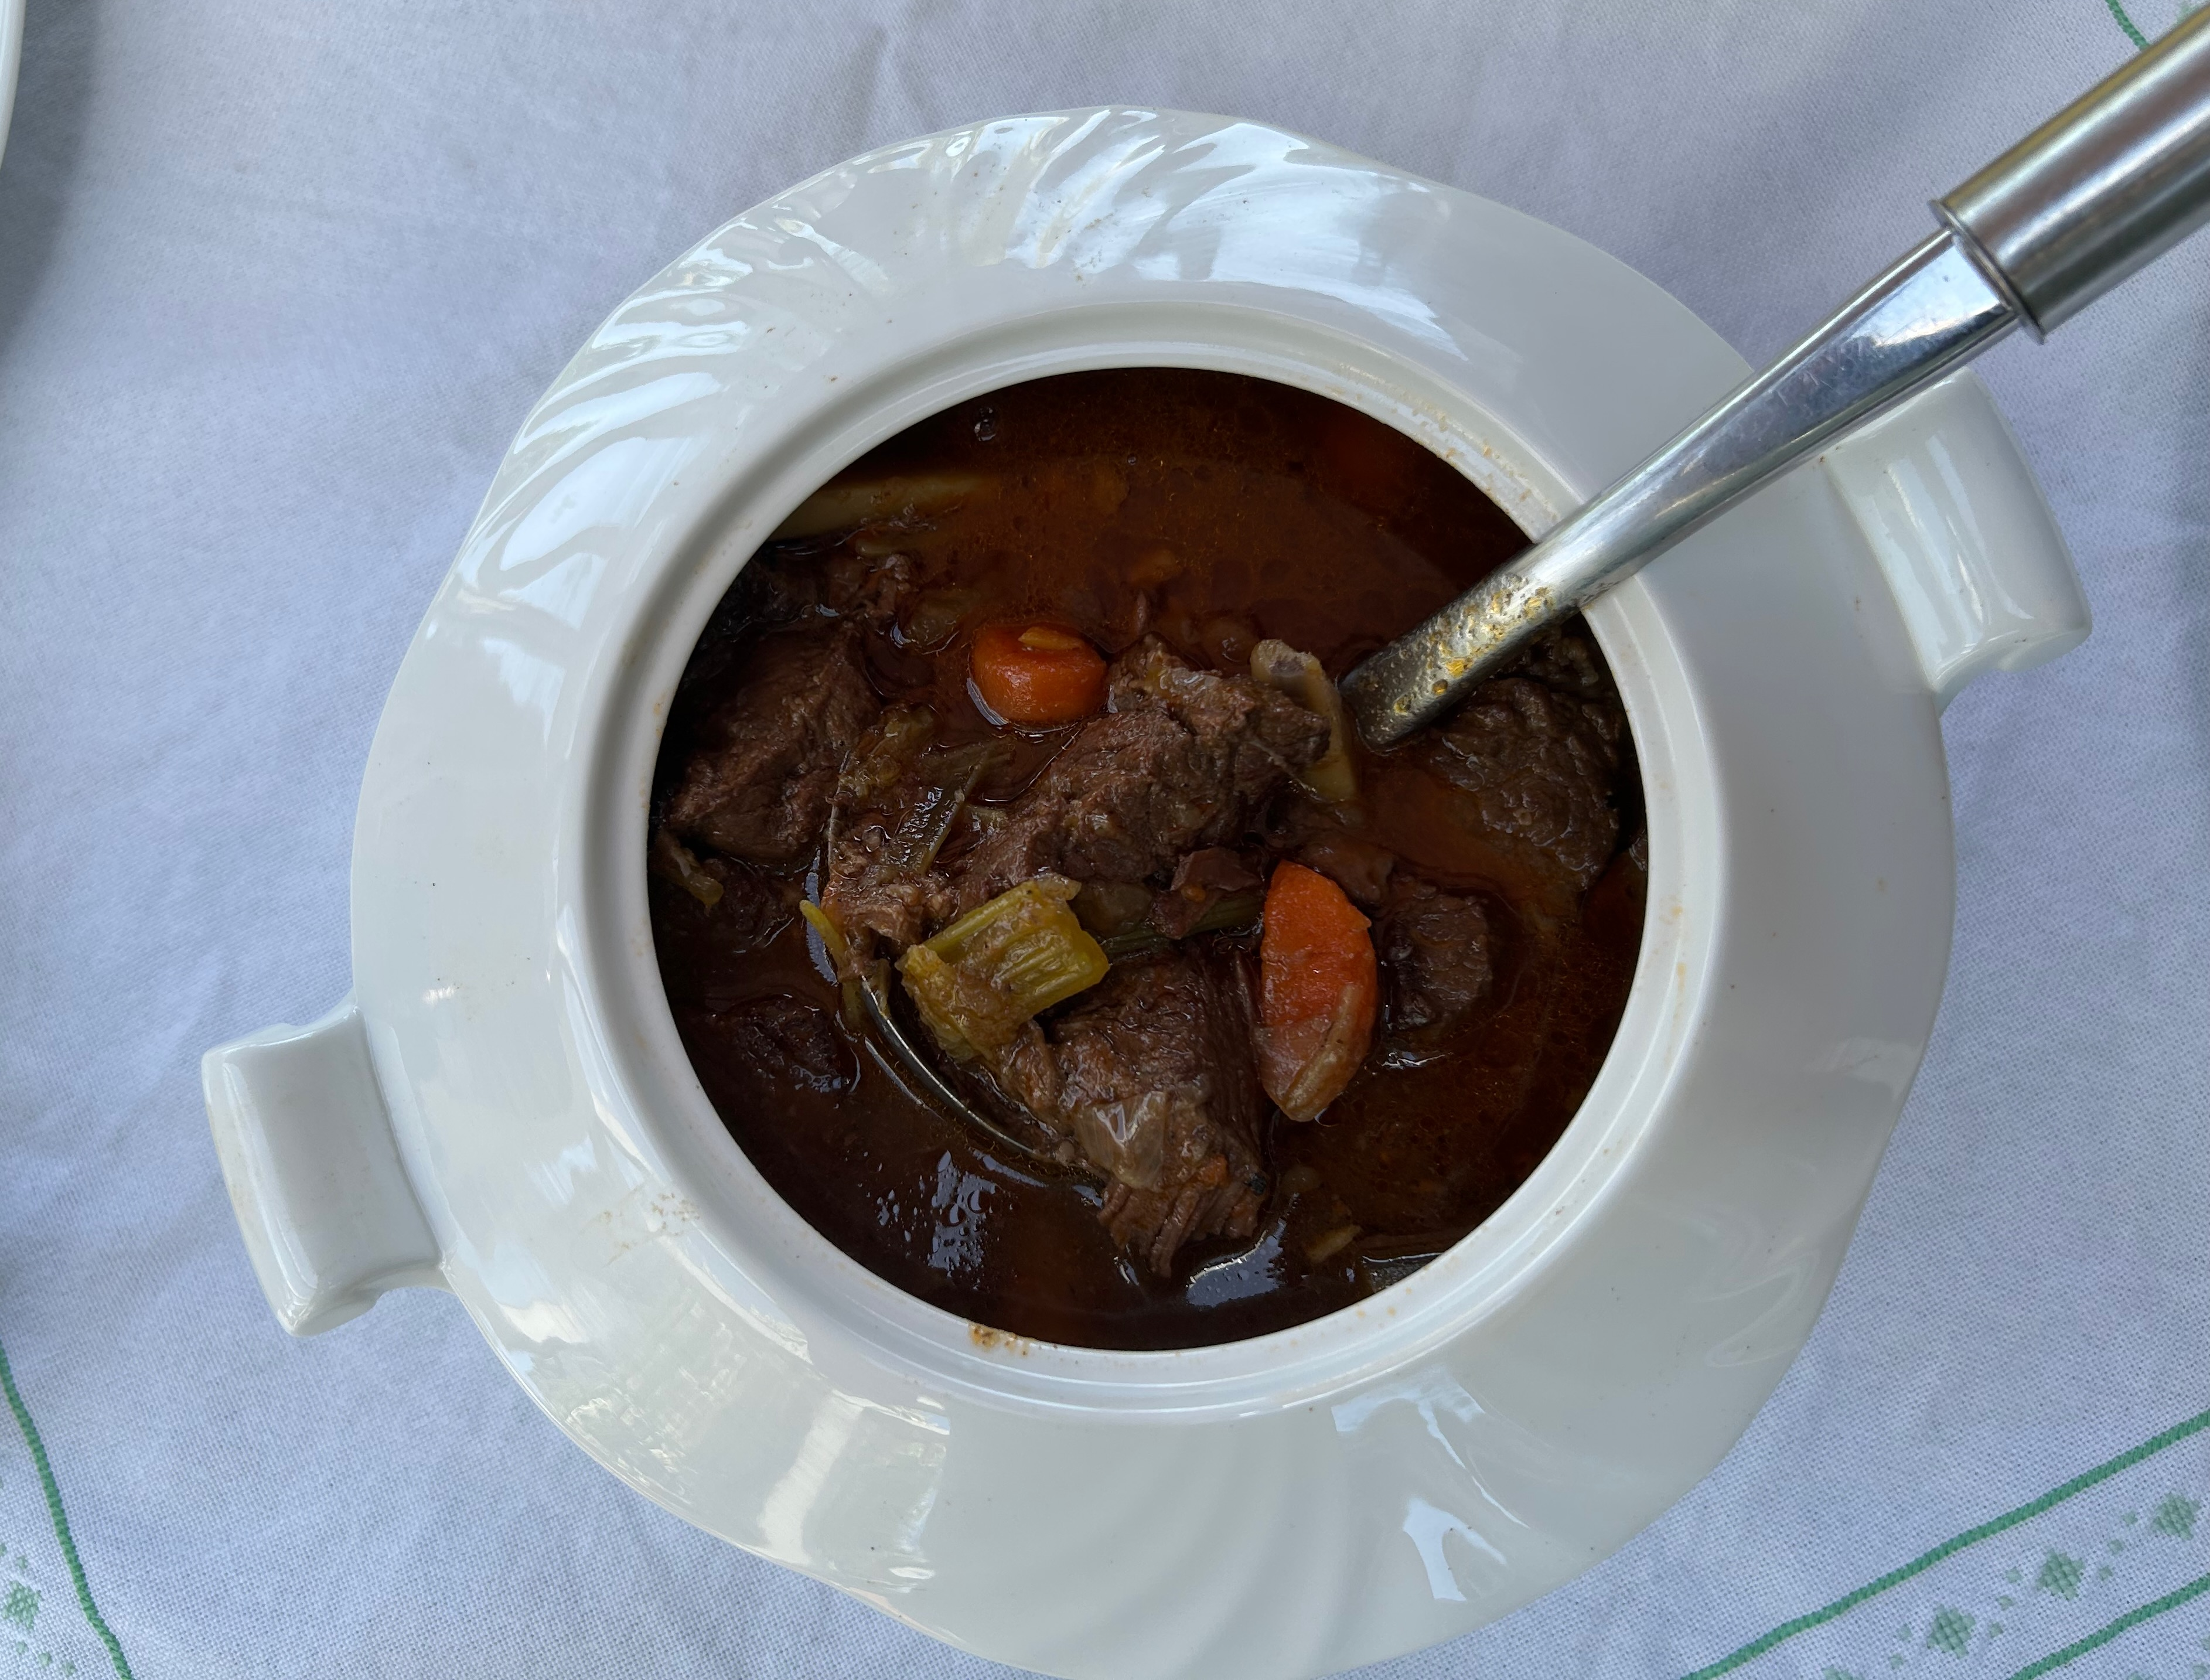
\includegraphics[width=1\linewidth]{pics/Irish_Stew}
		\captionof{figure}{Irish Stew}
		\label{fig:Irish_Stew}
	\end{minipage}
\end{figure}
\newpage


\section{Geflügel}

\subsection{Road Killed Chicken}

\paragraph{Geräte:}

\begin{itemize}[noitemsep]
	\item Kugelgrill
 	\item Gasgrill (min. 3 Brenner)
	\item Kamado Grill (Keramikgrill)
\end{itemize}

\paragraph{Zutaten für das Road Killed Chicken}

\begin{itemize}[noitemsep]
	\item Label rouge franz. Maishuhn
	\item Chicken Rub (Rezept siehe Kapitel~\ref{Chapter6} \vref{Chicken})
\end{itemize}

Wie wird das Hähnchen für „Road Killed Chicken“ vorbereitet?

Das ist wirklich einfach: Ihr legt das Hühnchen auf die Brustseite und 
schneidet mit einem Sägemesser oder einer Geflügelschere links und 
rechts neben dem Rückgrat komplett von oben nach unten durch. Den 
Knochenstrang könnt ihr dann einfach entnehmen (und möglicherweise 
mit anderen Fleischabschnitten zu Hühnerbrühe kochen). Wenn ihr das 
Huhn nun auseinandergeklappt auf die Innenseite legt, ist es ziemlich 
flach. Drückt gegebenenfalls nochmal fest mit der Hand aufs Brustbein, 
um es noch flacher zu machen. Der Vorteil dieser Methode ist, dass das 
Huhn gleichmäßig flach ist und daher schnell gart. Dadurch bleibt das 
Huhn schön saftig mit krosser Haut wie in 
Abbildung~\vref{fig:RoadKilledChicken}.

Den Grill (egal welchen Ihr einsetzen wollt) auf 180°C indirekte Hitze 
einstellen.
Das Huhn mit der Brustseite nach oben auf den Grill legen und bis zu 
einer Temperatur in der Keule vom 90°C grillen. Das Huhn vom Grill 
nehmen mit Salaten und Baguette servieren, lecker.
\newpage

\begin{figure}[htbp]
	\centering
	\begin{minipage}{1\textwidth}
		\centering
		\includegraphics[width=1\linewidth]{pics/Platthuhn_Teller}
		\captionof{figure}{Road Killed Chicken}
		\label{fig:RoadKilledChicken}
	\end{minipage}
\end{figure}
\newpage

\subsection{Buffalo (Chicken) Wings}
Die Buffalo Wings wurden in der Anchor Bar in Buffalo, New York in den 60 
Jahren das erste mal 
zubereitet. Die Wings wurden anfänglich 
noch als Snacks gereicht. Fanden aber mit wachsender Beliebheit schließlich 
den Weg auf die 
Speisekarte. Durch das entstehen der 
Sportsbars in denen die Wings serviert wurden fanden sie Verbreitung in den 
USA. Die Buffalo 
Wings sind seither untrennbar mit Football 
verbunden, ähnlich wie Hot Dogs mit Baseball. Durch diverse Fast Food-Ketten 
fanden sie bald 
weltweit Beachtung.

Die originalen Buffalo Wings wurden frittiert und danach in einer roten Chilisauce 
geschwenkt. 
Meistens wurde dafür Frank's Red Hot 
Sauce als Basis verwendet und mit Butter und weiteren Zutaten veredelt.

Ich stelle euch meine Interpretation der Buffalo Wings vor. 
Inspiriert von Michi von "`Einfach Grillen"' werde ich die Wings auf dem Grill 
unter Zugabe 
von Rauch zubereiten. 

Ich stelle euch außerdem noch drei Arten der Zubereitung der Buffalo Wings 
Sauce vor.

Lasst euch überraschen. Mo und ich halten diese Wings für the best Chicken 
Wings ever.


\paragraph{Geräte:}

\begin{itemize}[noitemsep]
	\item Kugelgrill
	\item Gasgrill
	\item Kamado Grill (Keramikgrill)
\end{itemize}

\paragraph{Zutaten für 2 Personen}

\begin{itemize}[noitemsep]
	\item 2 kg Hühnerflügel (bekommt man in der Regel ohne Spitzen, sollten die 
	Spitzen noch 
	dran sein, bitte entfernen)
	\item 12-15 g Salz
	\item Pfeffer
	\item 1 Päckchen Backpulver (1 je nach Hersteller 15 g bis 17 g)
	\item 1TL Cayennepfeffer
	\item 1,5 gestrichener TL Brauner Rohrzucker
\end{itemize}

Die Hühnerflügel werden in Flat und Drumstick geteilt, in dem sie am Gelenk 
auseinander ge
schnitten werden. Danach werden alle Teile 
trocken getupft (bitte nicht abwaschen) und in eine Schüssel gegeben. Die 
Gewürzmischung 
wird über die Wings gestreut und 
einmassiert. Diese werden dann auf einem Backblech ausgelegt und gekühlt. 
Durch das im Backpulver enthaltene Natron wird die Haut schön trocken, das ist 
die 
Voraussetzung, dass die Wings schön 
knusprig werden.

Den Grill für direkte und indirekte Hitze Vorbereiten und auf ca. 180°C einstellen. 
Dabei ist es 
egal ob Gas-, Holzkohle- oder Keramikgrill. 
Pellets, Chips oder Chunks zum Räuchern bereitstellen. Zu dem Gericht passen 
Buche, Apfel- 
oder Kirsche. Ich persönlich nehme die die 
Whiskey Wood Chips von Napoleon, diese haben ein unglaubliches Aroma.


Die Wings werden über der direkten Hitze scharf angegrillt und danach auf die 
indirekte Zone 
gelegt. Die Wings werden nun  ca. 40 
Minuten auf der indirekten Hitze gegrillt, bitte nicht den Rauch vergessen. 
Während dieser Zeit 
den Deckel bitte nicht lüften, ganz nach 
dem Motto "`if you looking, you ain't cooking"'. Nach 40 Minuten sollte sich das 
Fleisch leicht 
von den Knochen lösen lassen und die 
Wings sehr knusprig sein.

Während die Wings auf den Grill liegen widmen wir uns der Sauce.

Ich versprach euch drei Varianten:

\paragraph{Zutaten Sauce Variante 1}

\begin{itemize}[noitemsep]
	\item ca. 300 ml Frank's Red Hot Wings Sauce
\end{itemize}

Die Sauce im einem Topf erwärmen.

\paragraph{Zutaten Sauce Variante 2}

\begin{itemize}[noitemsep]
	\item 150 g Butter
	\item 2 EL Worcester Sauce
	\item 1 Zehe Knoblauch
	\item ca. 300 ml Frank's Red Hot Sauce
	\item 3 EL Weißweinessig
	\item 1 TL Cayennepfeffer
	\item 2 EL Paprikapulver, süß
	\item 1 Chili (optional)
\end{itemize}

\paragraph{Zutaten Sauce Variante 3}

\begin{itemize}[noitemsep]
	\item 16 Cayenne Chili
	\item 2 Habanero Red
	\item 380 ml Weißweinessig
	\item 2 Zehen Knoblauch
	\item 1 TL Salz
	\item 1 TL Knoblauchpulver
	\item 1 TL geräuchertes Paprikapulver
\end{itemize}

Buffalo Wings Sauce:

\begin{itemize}[noitemsep]
	\item 150 g Butter
	\item 1 EL Worcester Sauce
	\item 1 Zehe Knoblauch 
	\item 3 EL Weißweinessig
	\item 1 TL Kaschmir Chili-Pulver
	\item 1 EL Paprikapulver, süß
	\item 1 Chili (optional)
\end{itemize}

Den Strunk des Habanero und der Cayenne Chilis entfernen und die Schoten 
halbieren. Die Chilis mit den übrigen Zutaten 15 Minuten 
köcheln, mit dem Stabmixer pürieren und durch ein Sieb streichen. Diese Sauce 
mit den weiteren Zutaten zur Buffalo Wings Sauce 
weiterverarbeiten und erwärmen.

Die gegrillten Chicken Wings in der erwärmten Sauce (Variante 1 oder 2 oder 3) 
schwenken, nochmals auf den Grill legen, bis 
die Sauce angetrocknet ist. Die Wings anrichten und die übrige Sauce dazu 
reichen siehe Abbildung~\vref{fig:BuffaloWings}.

In einer Blindverkostung von 10 Familienmitgliedern wurde die Variante 3 mit 10 
von 10 Stimmen als beste Sauce befunden. Dafür danke ich 
herzlichst.                    
\newpage

\begin{figure}[htbp]
	\centering
	\begin{minipage}{1\textwidth}
		\centering
		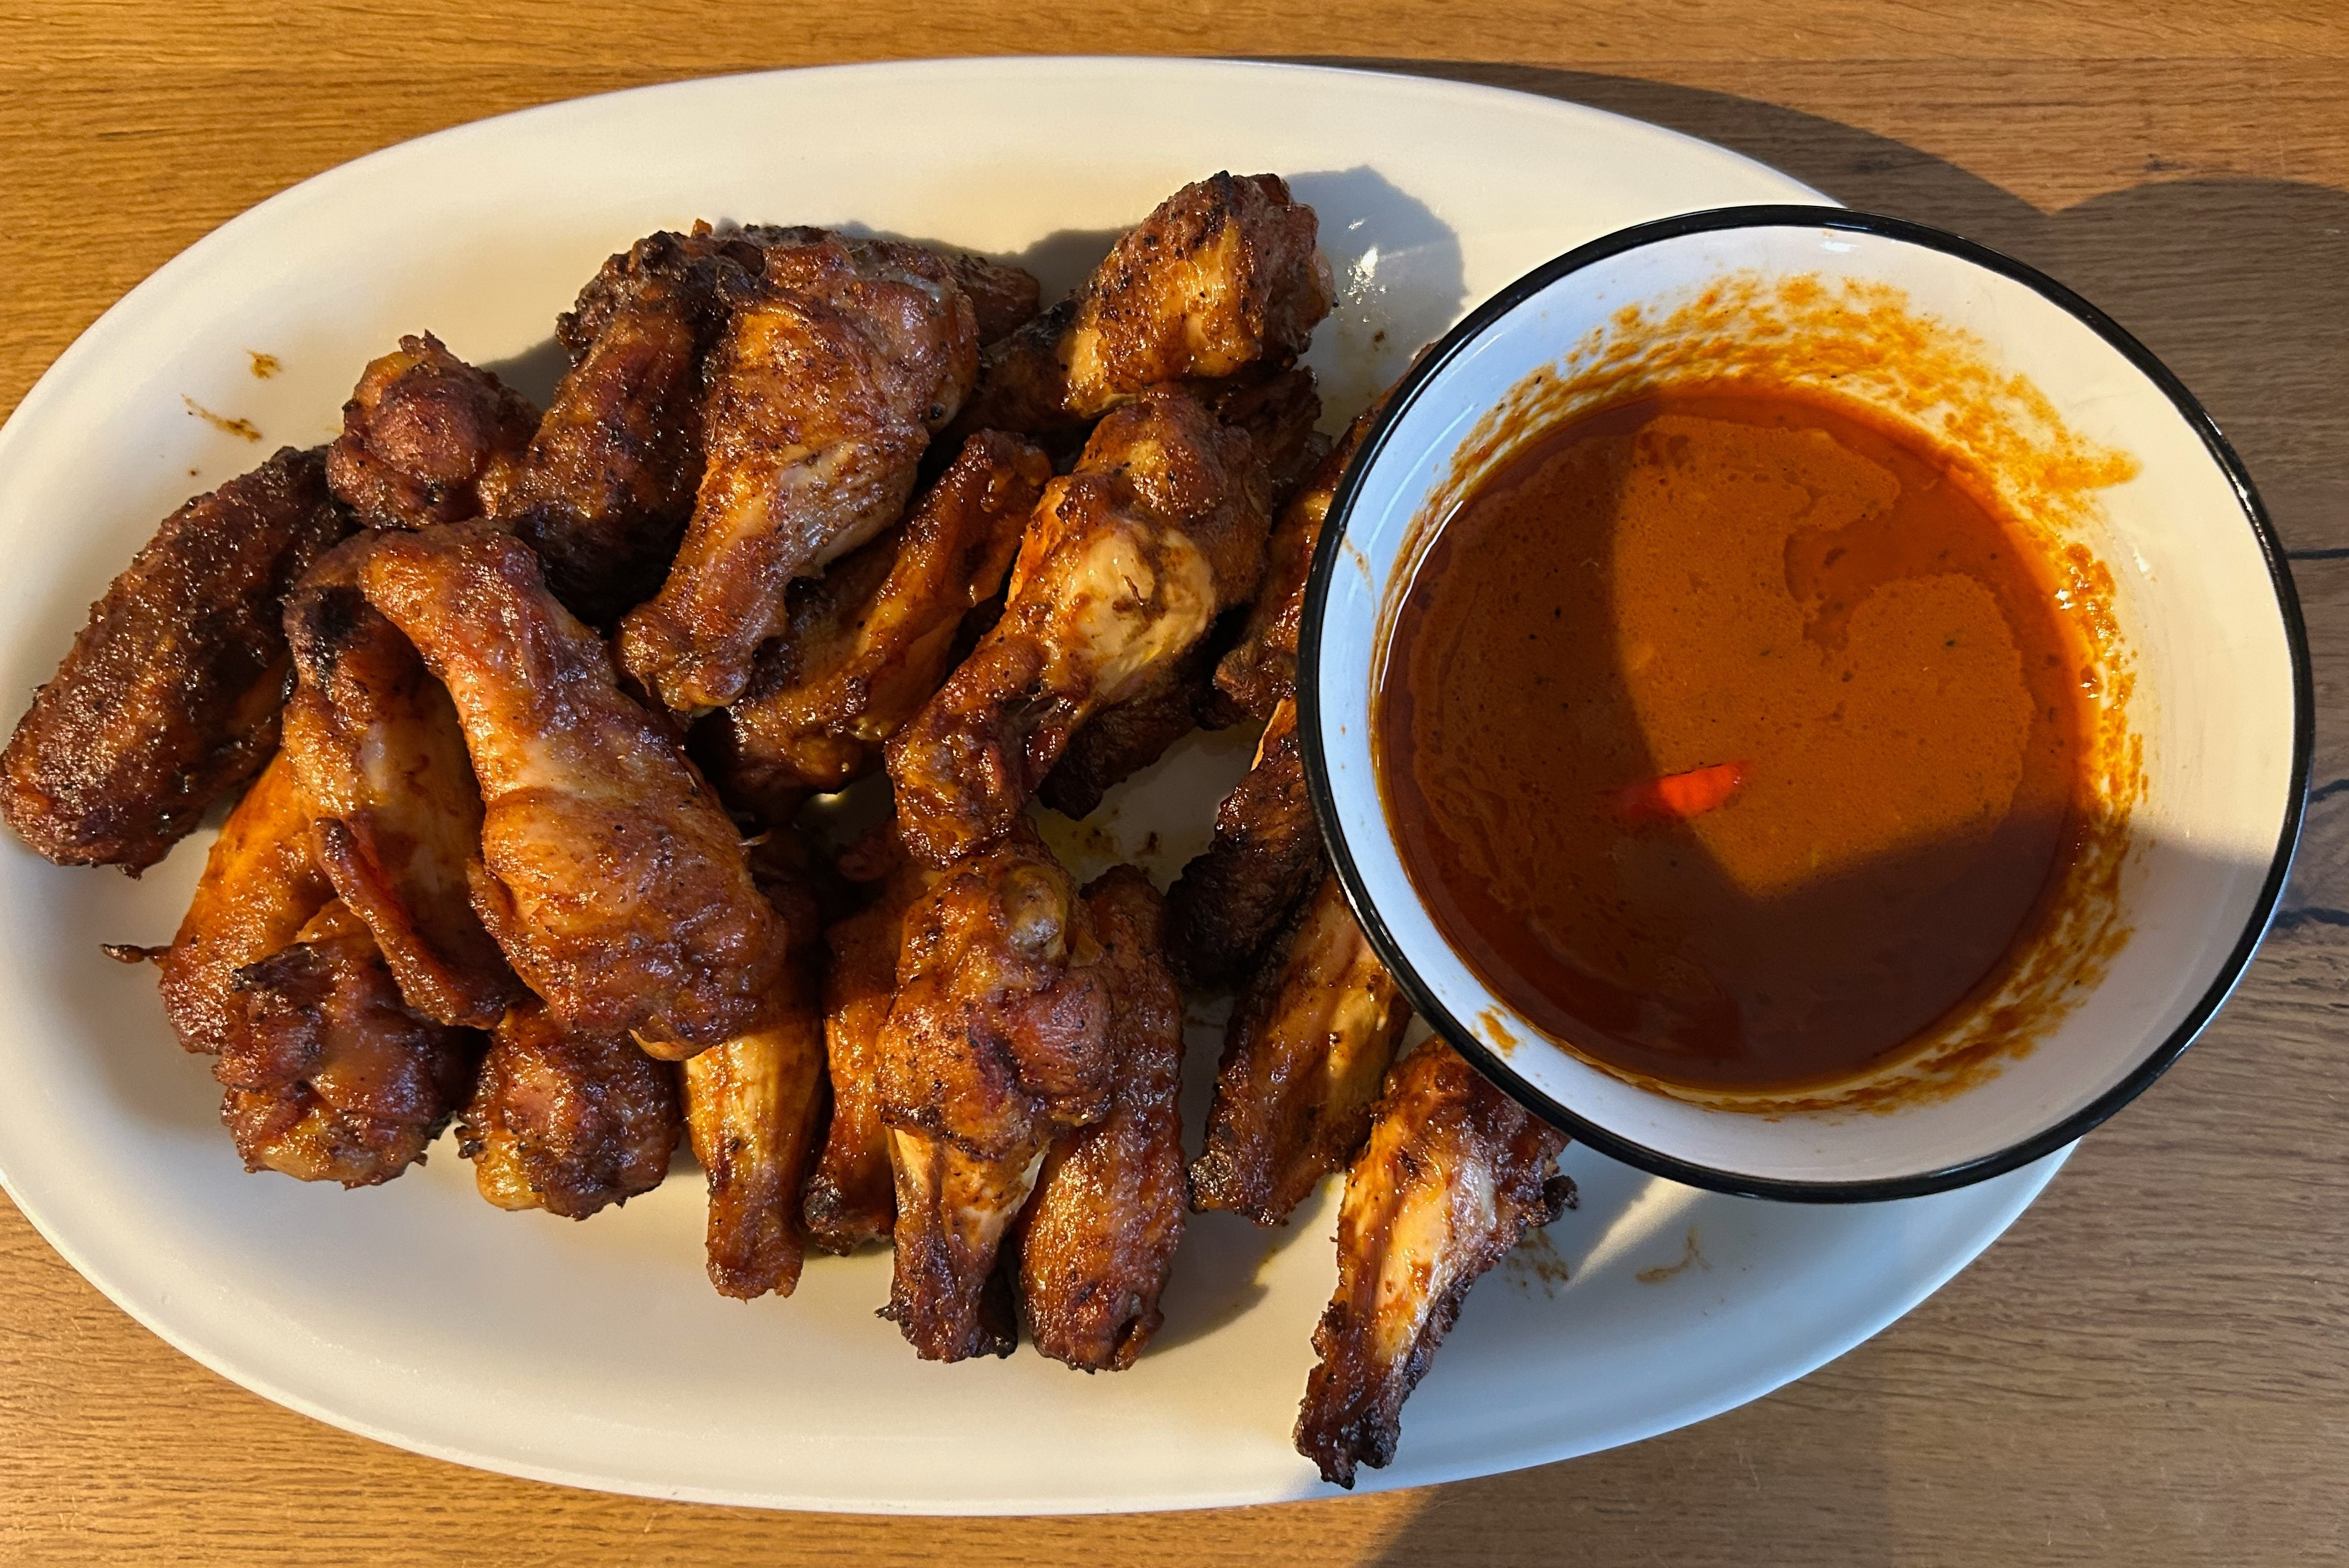
\includegraphics[width=.9\linewidth]{pics/Buffalo_Wings}
		\captionof{figure}{Buffalo Chicken Wings}
		\label{fig:BuffaloWings}
	\end{minipage}
\end{figure}
\newpage

\subsection{Helles Chili}\label{Helles Chili}

\paragraph{Geräte}

\begin{itemize}[noitemsep]
	\item Dutch oven
\end{itemize}

\paragraph{Zutaten}

\begin{itemize}[noitemsep]
	\item  500 g Hühner- oder Putenbrust
	\item 1 Gemüsezwiebel
	\item 1 chinesischer Knoblauch
	\item 1 Dose Mais (400 g)
	\item 2 Dosen Weiße Bohnen (400 g)
	\item 1 Grüne Paprikaschote
	\item 2 cl Veterano Brandy oder Goldener Tequila
	\item 1 EL Berberitze (für die Säure)
	\item 3-5 Lemondrop Chilis (je nach Geschmack)
	\item 50 ml Olivenöl
	\item 50 ml Sonnenblumenöl
	\item 20 g Weiße Schokolade
	\item 1 EL Gekörnte Brühe
	\item 1/2 TL Piment, ganz
	\item 1/2 TL Kardamom
	\item 1 TL geriebener Ingwer
	\item 1/2 TL Koriandersamen
	\item 1 Prise Zimt
	\item Salz \& Pfeffer
	\item 200 ml Wasser
\end{itemize}

\paragraph{Zubereitung}

Piment, Kardamom und Koriandersamen in einer Pfanne anrösten bis Knackgeräusche zu hören sind. Dann in eine Schüssel geben und nach dem Abkühlen die anderen Gewürze, bis auf Salz und Pfeffer zugeben, die Gewürze vermischen und zur Seite stellen.
Die Zwiebeln, die Chilis und den Knoblauch in Würfel schneiden und im Olivenöl andünsten. Zwischenzeitlich die Hühner- oder Putenbrust und die Paprikaschote in Würfel (ca. 1 cm Kantenlänge) schneiden und das Fleisch im Sonnenblumenöl scharf und kurz anbraten.
Die angedünsteten Zutaten zu dem Fleisch geben, nochmals bei starker Hitze rösten um Röststoffe zu entwickeln. Den Tequila oder Brandy zugeben, sobald der Alkohol verkocht ist mit dem Wasser ablöschen. Den Mais, die Berberitze  und den Paprika zugeben, das Ganze 15 Minuten bei mittlerer Hitze ohne Deckel köcheln lassen.  
Die Bohnen und die Gewürze zugeben und alles nochmals 15 Minuten ohne Deckel köcheln lassen.
Das Chili in einer Schüssel servieren und Weißbrot dazu reichen.


\section{Fisch}

\subsection{Sardinen vom Grill}

\paragraph{Geräte}

\begin{itemize}[noitemsep]
	\item Kugelgrill
	\item Kamado Grill
	\item Gasgrill
\end{itemize}

\paragraph{Zutaten}

\begin{itemize}[noitemsep]
	\item Sardinen, ausgenommen
	\item Salz \& Pfeffer
	\item Eine Zitronenscheibe pro Sardine
\end{itemize}

\paragraph{Zubereitung}

Den Gasgrill auf ca. 200°C vorheizen. Den Rost mit Trennspray einsprühen,  beim Einsprühen gibt es Stichflammen, da die Brenner eingeschaltet sind. Die Sardinen salzen und ca. eine Stunde liegen lassen. Danach die Sardinen auf den Grill legen und von jeder Seite ca. 3 Minuten, je nach Größe,  grillen. 

\begin{figure}[htbp]
	\centering
	\begin{minipage}{1\textwidth}
		\centering
		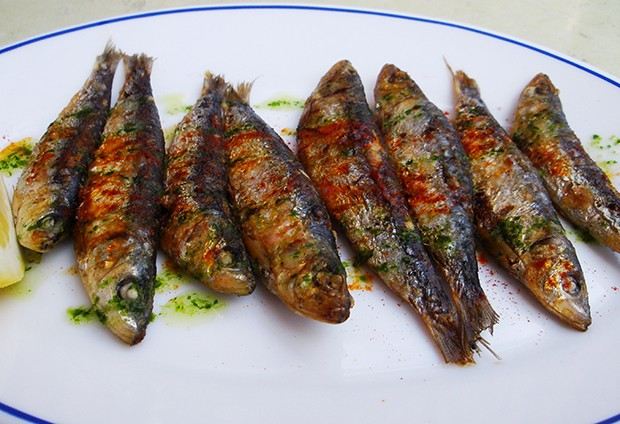
\includegraphics[width=.9\linewidth]{pics/Gegrillte_Sardinen}
		\captionof{figure}{Gegrillte Sardinen}
		\label{fig:Gegrillte_Sardinen}
	\end{minipage}
\end{figure}
\newpage

\subsection{Dorade Royal im Kartoffelbett}

\paragraph{Geräte}

\begin{itemize}[noitemsep]
	\item Gasgrill
\end{itemize}

\paragraph{Zutaten}

\begin{itemize}[noitemsep]
	\item 1 Dorade Royal pro Person
	
\end{itemize}

\paragraph{Zubereitung}

\subsection{Spanische Fischsuppe}

\paragraph{Geräte}


\paragraph{Zutaten}

\paragraph{Zubereitung}

\section{Meeresfrüchte}

\paragraph{Geräte}

\paragraph{Zutaten}

\paragraph{Zubereitung}


\subsection{Gegrillte Garnelen}

\paragraph{Gräte}

\paragraph{Zutaten}

\paragraph{Zubereitung}


\subsection{Ingwer-Garnelen vom Grill}

\paragraph{Geräte}

\paragraph{Zutaten}

\paragraph{Zubereitung}


\subsection{Pulpotentakeln vom Grill}

\paragraph{Geräte}

\paragraph{Zutaten}

\paragraph{Zubereitung}


\subsection{Dreierlei Muscheln von der Plancha}

\paragraph{Geräte}

\paragraph{Zutaten}

\paragraph{Zubereitung}%Tierisch Gut
%!TEX root = Vorlage_Buch.tex
\chapter{Gemüse und Pilze die unterschätzten Darsteller in der Küche}\label{Chapter3}

\lettrine[lines=3]{G}{emüse mach Spass, wetten dass?} In diesem Kapitel möchte ich euch zeigen, dass Gemüse zu Schade ist um als Beilage oder zu Kaninchenfutter degradiert wird sondern richtiges Soulfood, nicht nur für Veggies, ist. Es ist bunt, es ist vielseitig, es ist knackig (wenn es nicht getötet wird) und es ist vor allem vielseitig. Lassen wir uns auf das Experiment Gemüse ein.  In diesem Kapitel werden auch Pilze betrachtet, sie gehören allerdings weder zur Flora noch zur Fauna, sondern bilden ihr eigenes Reich. Ich habe die Pilze trotzdem hier aufgenommen, das ein eigenes Kapitel für diese Buch nicht gewinnbringend wäre.

\section{Gemüse als Beilage}

\subsection{Weißer Spargel, gedämpft}

\paragraph{Geräte}

\begin{itemize}[noitemsep]
	\item Holzkohlegrill
	\item Gasgrill
	\item Kamado Grill
\end{itemize}

\paragraph{Zutaten}

\begin{itemize}[noitemsep]
	\item 1,5 kg Spargel, geschält
	\item Saft einer Zitrone
	\item Olivenöl, genau soviel wie Zitronensaft
	\item 1 gute Prise Salz
	\item 1 gute Prise Zucker
	\item 3 Bögen Backpapier
	\item Aluminiumfolie
\end{itemize}
	
\paragraph{Zubereitung}
Den Zitronensaft, das Öl, das Salz und den Zucker mit einem kleinen Schneebesen 
verrühren. Je ein Drittel der Spargel auf einen Bogen Backpapier nebeneinander 
legen und mit einem Drittel der Marinade beträufeln. Das Backpapier 
einschlagen, sodass dichte Päckchen entstehen. Diese Päckchen in Alufolie 
einschlagen und bei ca. 200°C 20-25 Minuten auf der indirekten Zone bissfest 
garen. Die Spargel mit Lavendelbutter Kapitel~\ref{Chapter6} \vref{LavButter} 
bestreichen und servieren. Die Aromatik ist unbeschreiblich.

\subsection{Gegrillte Blumenkohlschnitzel}

\paragraph{Geräte}

\begin{itemize}[noitemsep]
	\item Gasgrill mit Plancha
\end{itemize}

\paragraph{Zutaten}

\begin{itemize}[noitemsep]
	\item 1 großer Blumenkohl
	\item grobes Himalaya-Salz aus der Mühle
	\item Olivenöl
\end{itemize}

\paragraph{Zubereitung}

Den Grill auf ca. 200°C vorheizen. Den Blumenkohl in ca. 2 cm dicke 
Scheiben schneiden. Die Blumenkohlscheiben mit Olivenöl beträufeln und 
salzen. Die Blumenkohlschnitzel auf der Plancha von beiden Seiten anbraten, 
bis sie stark gebräunt sind. Warm servieren und eventuell eine Vinaigrette 
dazu reichen.

\subsection{Gegrillter Rosenkohl}

\paragraph{Geräte}

\paragraph{Zutaten}

\paragraph{Zubereitung}

\subsection{Spitzkohl vom Grill}

\paragraph{Geräte}

\paragraph{Zutaten}

\paragraph{Zubereitung}

\paragraph{Wurzelgemüse aus dem Grillkorb}

\paragraph{Geräte}

\paragraph{Zutaten}

\paragraph{Zubereitung}

\subsection{Mediterranes Gemüse vom Grill}

\paragraph{Geräte}

\paragraph{Zutaten}

\paragraph{Zubereitung}



\section{Pilze und was sich daraus machen lässt}

\subsection{Steinpilz-Burger mit Kartoffelstroh}

\paragraph{Geräte}

\begin{itemize}[noitemsep]
	\item Gasgrill mit Plancha
	\item Fritteuse oder Airfryer
	\item Spiralschneider
\end{itemize}

\paragraph{Zutaten}

\begin{itemize}[noitemsep]
	\item 200 g Steinpilze
	\item 200 g Zwiebeln
	\item 1 Chinesischer Knoblauch
	\item Salz \& Pfeffer
	\item 1 Schuss süße Sahne
	\item 1 Kartoffel
	\item 1 Brioche-Bun
	\item Salat
	\item Orangen-Mayonnaise
\end{itemize}

\paragraph{Zubereitung}



%Gemüse
%!TEX root = Vorlage_Buch.tex
\chapter{Leckeres aus dem Holzbackofen}\label{Chapter4}
\lettrine[lines=3]{D}{er Holzbackofen} ist eine echte Bereicherung für das 
Outdoor-Kochvergnügen.
Die Einsatzmöglichkeiten sind schier unerschöpflich. Fast alles das auf
dem Herd oder dem Grill gemacht wird, ist auch im Backofen möglich. Ob
Fleisch, Fisch, Gemüse, Pizzen, Brote oder Desserts das alles gelingt im 
Holzbackofen. Der Kreativität wird keine Grenzen gesetzt. Das Charmante an
dieser Zubereitungsmethode ist die lange Haltezeit der Temperatur. Pizzen
werden jenseits der 300 ℃ gebacken, danach kann locker noch ein 
Holzofenbrot gebacken werden. So kann die Restwärme noch sinnvoll genutzt
werden.

\begin{figure}[htbp]
	\centering
	\begin{minipage}{1\textwidth}
		\centering
		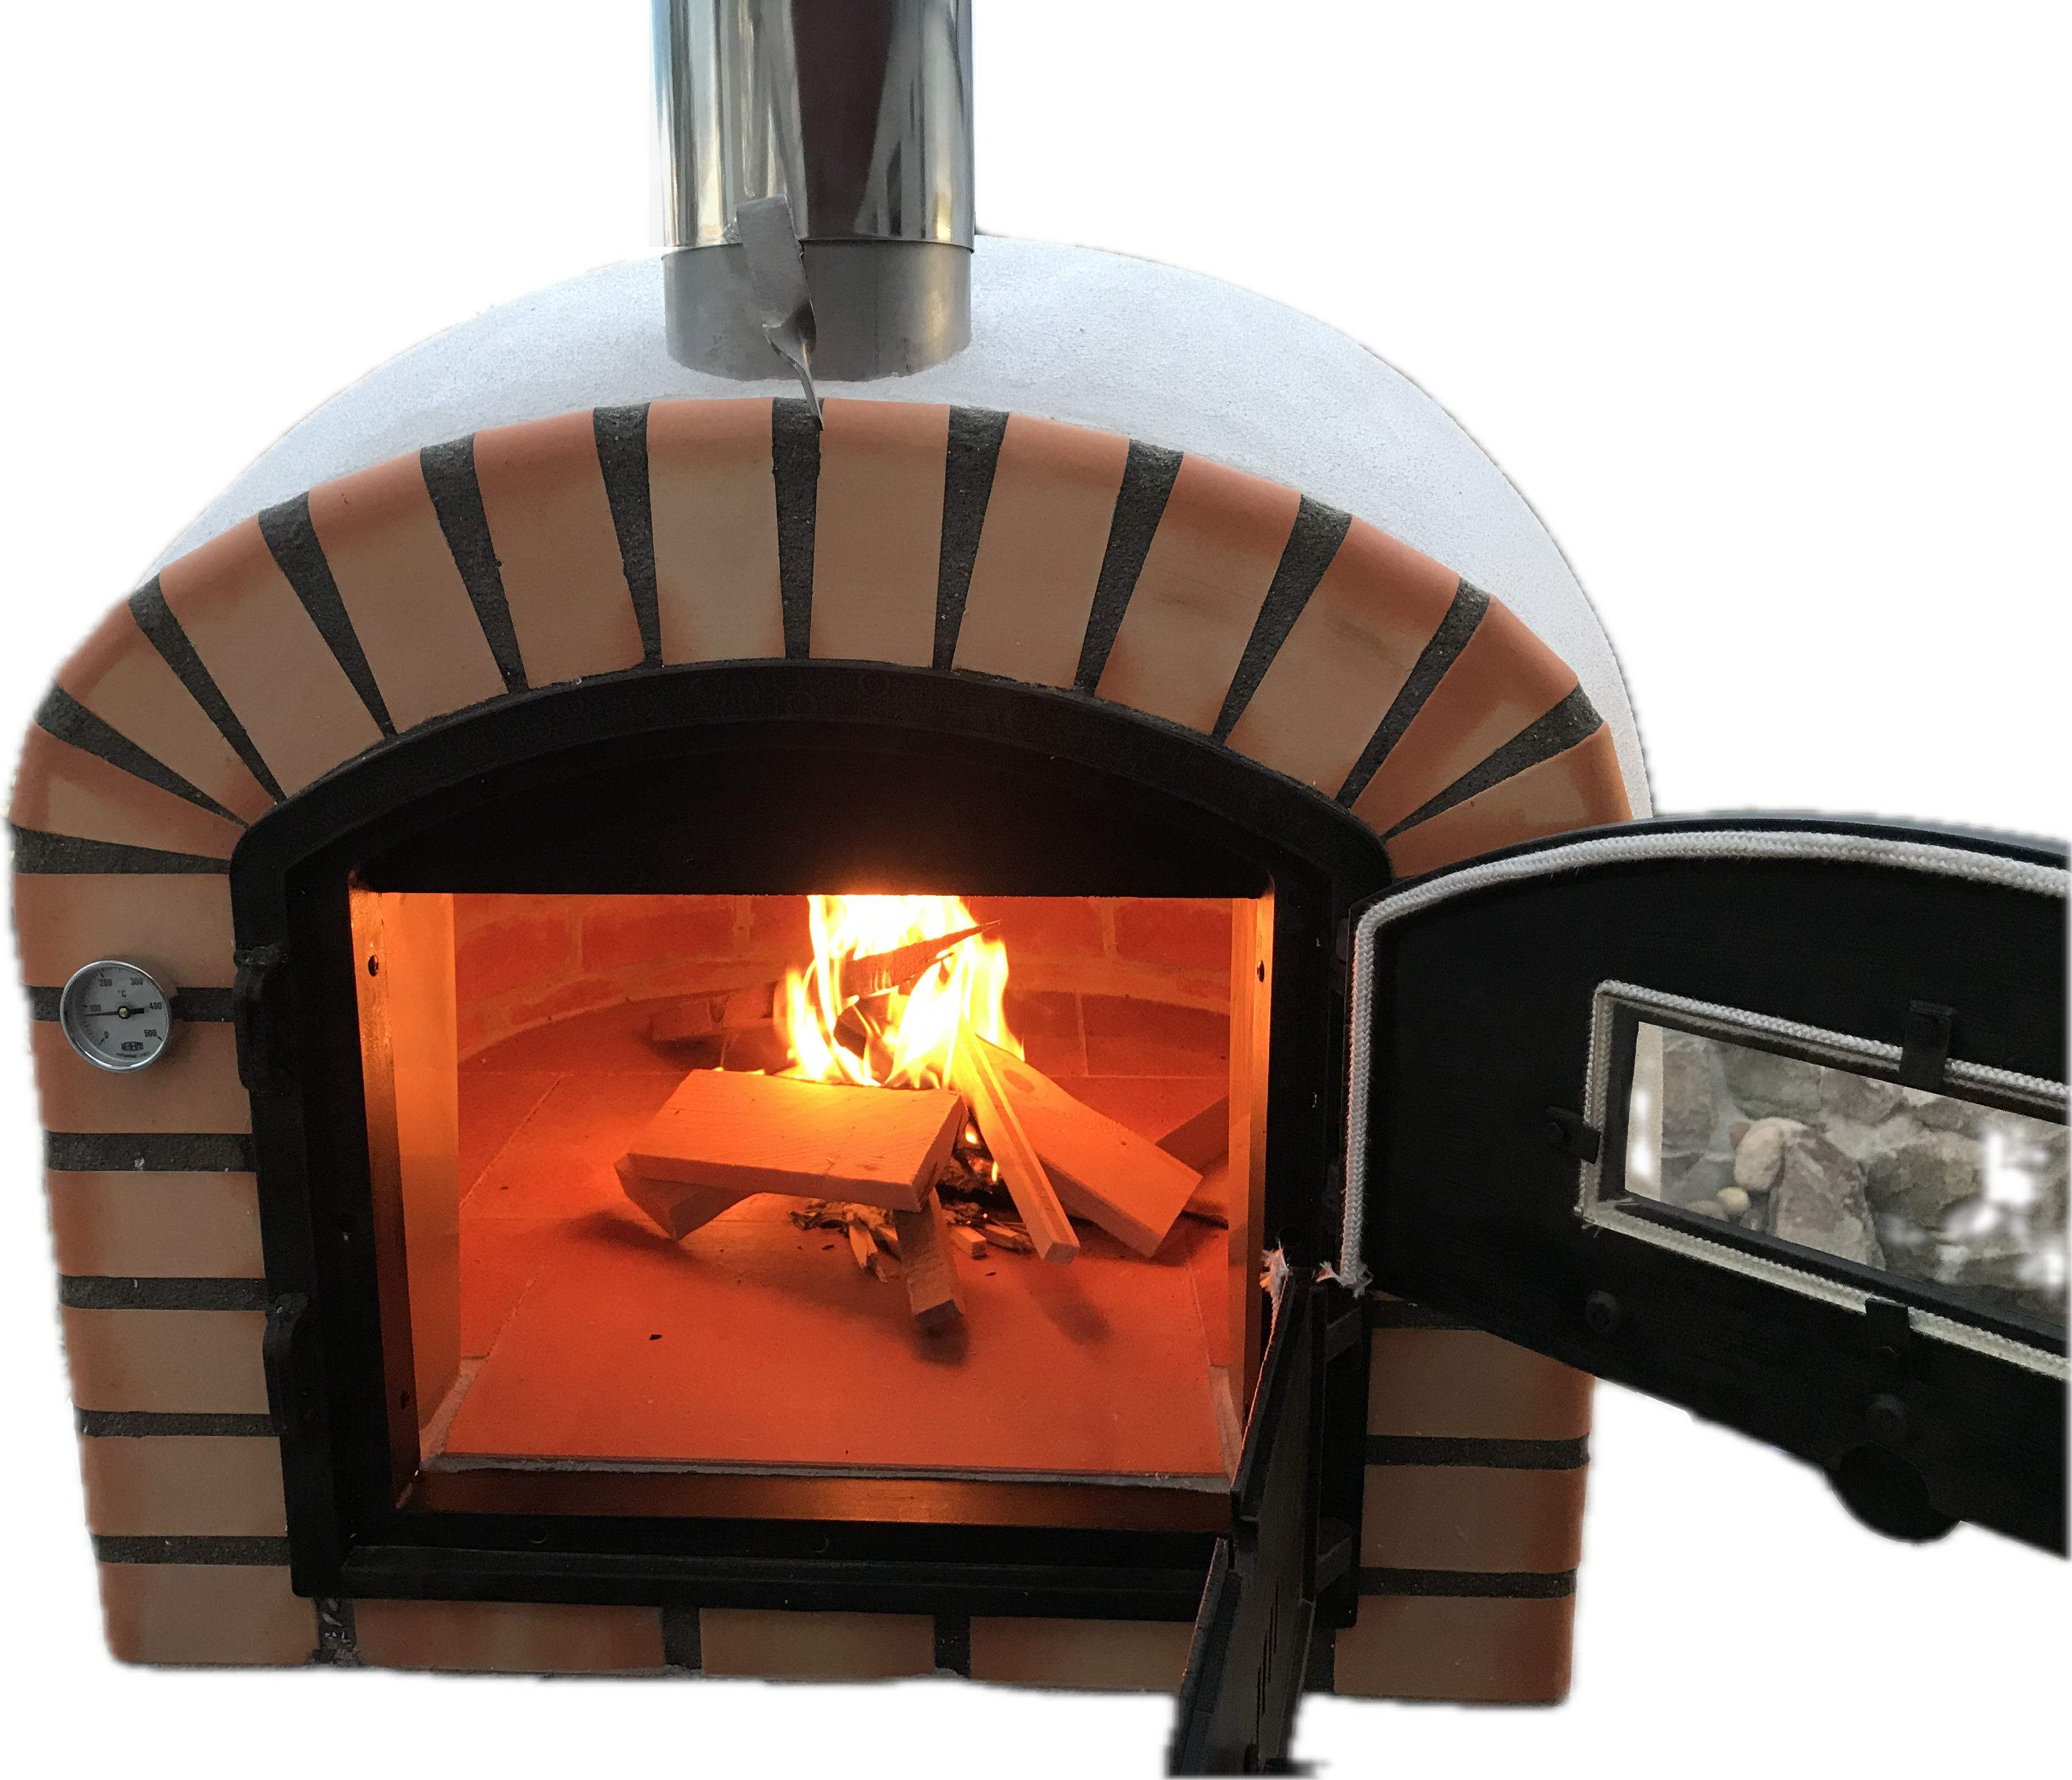
\includegraphics[width=.9\linewidth]{pics/Backofen}
		\captionof{figure}{HolzBackofen}
		\label{fig:Backofen}
	\end{minipage}
\end{figure}
\newpage

\section{Teige und was sich daraus machen lässt}

\subsection{Eine echt leckere Pizza}

\paragraph{Geräte}

\begin{itemize}[noitemsep]
	\item Holzbackofen
	\item Kenwood Cooking Chef
\end{itemize}

\paragraph{Zutaten Teig}

\begin{itemize}[noitemsep]
	\item 1 kg Mehl (Type 00 mit mindestens 12\% Eiweiß)
	\item 650 g kaltes Leitungswasser (Anfänger 600 g, weil leichter zu 
	verarbeiten)
	\item 25 g feines Salz
	\item 15 g Olivenöl
	\item 2 g frische Hefe
\end{itemize} 

\paragraph{Zutaten Pizzasoße}
 
\begin{itemize}[noitemsep]
	\item 500 g frische Tomaten
	\item 500 g passierte Tomaten aus der Flasche (hier von Mutti)
	\item 2 große Zwiebeln
	\item 2 Stück chinesischer Knoblauch
	\item 50 ml Olivenöl
	\item Salz
	\item je nach Geschmack Kräuter
\end{itemize}

\paragraph{Zubereitung }
Das Mehl in einer Rührschüssel vorlegen. Von dem Wasser ca. 100 ml 
abnehmen um die Hefe aufzulösen. Den Rest des Wassers zu dem Mehl 
geben 
und das Ganze mit einem Kochlöffel verrühren bis das gesamte Wasser 
aufgenommen wurde. Den Teig  abdecken und 30 Minuten ruhen lassen. Nach 
dem Ruhen das Olivenöl und das Wasser mit der aufgelösten Hefe zugeben und 
alles kneten, bis das Wasser und das Öl aufgenommen wurde, nun das Salz 
zugeben und den Teig fertig kneten ca. 15 Minuten. Da kann natürlich auch in 
einer Küchenmaschine erledigt werden. Knetzeit ca. 6 Minuten bei mittlerer 
Geschwindigkeit.
Den Teig in der Rührschüssel belassen und diese mit Frischhaltefolie 
verschließen. Den Teig 24 Stunden im Kühlschrank gehen lassen. Den Teig 
nach 24 Stunden aus der Schüssel nehmen, kurz durchkneten und in 6 
gleichmäßige Teiglinge teilen. Die Teiglinge zu Kugeln formen, in eine 
Auflaufform legen, diese mit Frischhaltefolie verschließen und nochmals 24 
Stunden im Kühlschrank gehen lassen. 

\paragraph{Zubereitung Tomatensoße}
Die Zwiebeln klein schneiden und im Olivenöl andünsten, nach einiger Zeit den 
gehackten Knoblauch zugeben. In der Zwischenzeit die frischen Tomaten in 
Stücke schneiden und zusammen mit den passierten Tomaten zu den 
angedünsteten Zwiebeln geben und köcheln lassen bis die Tomaten verkocht 
sind. Je nach Geschmack die Soße stückig lassen oder durch ein Sieb streichen.
Falls gewünscht Kräuter zugeben und mit Salz abschmecken.

\paragraph{Zubereitung Pizza}
Die Teiglinge aus der Form nehmen und von der Mitte heraus flach drücken, 
darauf achten, dass die Luft nicht aus den Rand gedrückt wird. Wenn der Boden 
die richtige Größe hat mit Tomatensoße bestreichen, nach Belieben belegen 
und bei mindestens 300°C im Holzbackofen backen.
\newpage

\begin{figure}[htbp]
	\centering
	\begin{minipage}{1\textwidth}
		\centering
		\includegraphics[width=1\linewidth]{pics/Pizza}
		\captionof{figure}{Pizza aus dem Holzbackofen}
		\label{fig:Pizza}
	\end{minipage}
\end{figure}
\newpage


\subsection{Brioche Buns}\label{BriocheBun}
Die Kunst ist es ein Bun herzustellen, der nicht zäh sondern schön mürbe ist. Er darf aber nicht zu schnell durchsuppen und sollte nicht in der 
Hand zerbröseln. Diese Eigenschaften in einem Brioche Buns zu vereinen kostet einiges an Experimentierarbeit. Zumal der Bun auch nicht 
trocken oder strohig werden darf.
Ich habe hier mein Rezept an ein Rezept aus dem Buch "Burger unser" (erschienen im Callwey Verlag, hier der Link zur in Leder gebunden Limited Edition \url{https://www.callwey.de/buecher/burger-unser-limited-edition/}) angelehnt, das für mich als gelernten Bäcker dem perfekten Brioche Bun  wohl am nächsten kommt.

\paragraph{Geräte}

\begin{itemize}[noitemsep]
	\item Holzbackofen
	\item Kenwood Cooking Chef
\end{itemize}

\paragraph{Zutaten}

\begin{itemize}[noitemsep]
	\item 3 EL Milch (3,8\% Fett)
	\item 50 g Rohrzucker
	\item 380 g Mehl, Type 550
	\item 1/2 Würfel frische Hefe
	\item 1 großes Ei
	\item 35 g warme Butter
	\item 45 g Mehl, Type 405
	\item 9 g Himalaya-Salz
	\item 240 ml Wasser
\end{itemize}

\paragraph{Zubereitung}

Milch auf ca. erwärmen nicht erhitzen, in eine Schüssel geben 1 EL Zucker und 1 EL Mehl
zugeben. Die Hefe hinein bröseln und alles verrühren. Stehen lassen
bis sich Blasen bilden. 
Die weiche Butter mit beiden Mehlsorten und Salz mischen bis eine streuselartige
Masse entsteht. Anschließend die Hefe-Milch-Mischung, Wasser und das Ei
langsam ein arbeiten. Die Küchenmaschine auf die mittlere Stufe einstellen und 
den Teig für ca. 8 Minuten kneten. Den Teig abdecken und 1-2 Stunden stehen lassen
bis sich das Volumen verdoppelt hat (Stockgare).
Nach der Stockgare den Teig auf der leicht bemehlten Arbeitsfläche in 8 gleiche Stücke
teilen. Die 8 Teile in schöne Kugeln formen, auf ein Backblech mit genügend Abstand legen
und eine Stunde liegen lassen, bis das Volumen verdoppelt hat (Stückgare).

Wenn die Buns aufgegangen sind mit einer Mischung aus 1 Eiklar, 1 EL Wasser und einer 
Prise Salz einstreichen. Dazu einen Silikonpinsel benutzen. Die Buns mit einem beliebigen
Topping, ich bevorzuge Sesam mit seinem unvergleichlichem nussigen Aroma, bestreuen
und 15-20 Minuten bei 200°C im Holzbackofen backen, bis die Oberfläche goldbraun ist.

\subsection{Kartoffel-Bun}
Der Kartoffel-Bun ist in Hinsicht der Luftigkeit und Stabilität die beste Alternative. Dieser 
Bun wird in den USA und in Kanada als Standard eingesetzt. Dieser Teig ist nicht so leicht 
wie der Brioche-Teig zu handhaben, ist allerdings deutlich luftiger. Es schmeckt auch 
weniger süßlich und ist für saftige Burger die erste Wahl. Auch dieses Rezept habe ich
an ein Rezept aus der selben Quelle wie das des Brioche Buns angelehnt.

\paragraph{Geräte}

\begin{itemize}[noitemsep]
	\item Holzbackofen
	\item Kenwood Cooking Chef
	\item Kartoffelstampfer oder Spätzlepresse
\end{itemize}

\paragraph{Zutaten}

\begin{itemize}[noitemsep]
	\item 300 ml Milch (3,8\% Fett)
	\item 1/2 Würfel frische Hefe
	\item 70 g brauner Zucker
	\item 300g Mehl, Type 405
	\item 200 g gekochte mehlige Kartoffeln (vom Vortag)
	\item 250 g Mehl, Type 550
	\item 10 g Himalaya-Salz
	\item 1 großes Ei
	\item 80 g Butter, weich
\end{itemize}

\paragraph{Zubereitung}

Die Milch auf erwärmen nicht erhitzen, in eine Schüssel geben 1 EL Zucker, 1 EL Mehl
und die Hefe zugeben und alles verrühren. Stehen lassen bis sich Blasen bilden. 

Die gekochten und geschälten Kartoffeln stampfen, bis keine groben 
Stücke mehr vorliegen oder durch eine Spätzlepresse drücken, aber niemals mit einem 
Handmixer verrühren, weil sich dadurch langkettige Moleküle bilden und die Kartoffeln
 Fäden ziehen. Die Kartoffeln zusammen mit der Hefe-Milch-Mischung, 
dem gesamten Mehl, dem Zucker, dem Salz und dem Ei in eine Küchenmaschine geben. 
Auf langsamer Stufe kneten bis ein grober Teig entsteht. 

Jetzt die Butter nach und nach einarbeiten, dabei die Küchenmaschine auf mittlere Stufe 
stellen. Anschließend die Küchenmaschine auf die höchste Stufe  einstellen und den 
Teig für 10 Minuten kneten. Den Teig in der Schüssel belassen, abdecken und für 1 bis 1,5
Stunden stehen lassen. Das Volumen sollte sich bis dahin verdoppelt haben (Stockgare).

Den Teig aus der Schüssel nehmen und gut kneten, dass die Luft entweicht. Den Teig 
mit den Händen flachdrücken und einschlagen, den Vorgang ein bis zweimal wiederholen.
Danach in 12 gleichmäßige Teile teilen und zu schönen kompakten Kugeln formen.

Die 12 Kugeln auf ein Backblech mit mit genügend Abstand legen und eine Stunde liegen
lassen, bis sich das Volumen verdoppelt hat (Stückgare).

Wenn die Buns aufgegangen sind mit einer Mischung aus 1 Eiklar, 1 EL Wasser und einer 
Prise Salz einstreichen. Dazu einen Silikonpinsel benutzen. Die Buns mit einem beliebigen
Topping, Schwarzkümmel mit ein wenig Salz ist auch ein schmackhaftes Topping mit einer
tollen Aromatik und 15-20 Minuten bei 200°C im Holzbackofen backen, bis die 
Oberfläche goldbraun ist.
%Leckeres aus dem Holzbackofen
%!TEX root = Vorlage_Buch.tex
\chapter{Beilagen und Snacks}\label{Chapter5}
\lettrine[lines=3]{BBQ}{bedeutet für mich} nicht nur Fleisch oder 'ne Rote im Brötchen. BBQ ist kochen und im Idealfall auch genießen im 
Freien. Fast alles was in der Küche im Haus zubereitet werden kann, kann auch in der Außenküche zubereitet werden.  Deshalb werde ich 
hier auch einige Rezepte vorstellen die von Oma gekocht wurden, bevor es jemanden gab der Barbecue (/ˈbɑː.bɪ.kjuː/)  aussprechen konnte.

Unter dem Punkt "`Ä Gosch voll"' werden wir Rezepte für kleine Happen kennenlernen.  Diese Häppchen sind mundgerecht und können als Amuse Gueule, 
zwischen den Gängen, als Dessert oder einfach als Fingerfood gereicht werden. In diesen Happen wird alles verpackt, das benötigt wird um Kleines ganz groß werde zu 
lassen. Also gehen wir es an.  

\section{Ä Gosch voll,}
besser beschreiben kann man die Kleinigkeiten nicht. Es ist wie im wirklichen Leben, die kleinen Dinge machen die meiste Arbeit, sorgen aber auch für den Größten 
Wow-Effekt. Daher bitte ein wenig Zeit einplanen, oder so viel möglich am Vortag vorbereiten. 

\subsection{Tiroler Schlutzkrapfen}

Schlutzkrapfen sind eine Nudelspezialität aus Tirol und werden aus einer 
Mischung von Roggen- und Weizenmehl hergestellt. Der Name leitet sich von 
"`Schluzen"' 
ab, was soviel wie Rutschen oder Gleiten bedeutet.

\paragraph{Geräte}

\begin{itemize}[noitemsep]
	\item Teigmaschine oder Hände
	\item Nudelmaschine
	\item Holzkohlegrill, Gasgrill oder Keramikgrill
\end{itemize}

\paragraph{Zutaten für die Schlutzkrapfen}

\begin{itemize}[noitemsep]
	\item 125 g Weizenmehl (hier Type 405)
	\item 125 g Roggenmehl (hier Type 997)
	\item 2 Eier
	\item 30 g Butter
	\item 2 L Wasser
	\item 1 TL Salz (hier Himalaya Salz)
\end{itemize}

\paragraph{Zubereitung}

Die beiden Mehlsorten mit dem Salz in einer Schüssel mischen. Die Butter zerlassen und mit den Eiern, dem Wasser hinzugeben. Das 
ganze mit der Küchenmaschine oder den Händen zu einem glatten Teig kneten. In ein Küchentuch einschlagen und 30 Minuten ruhen 
lassen.

\paragraph{Zutaten für die Füllung}

\begin{itemize}[noitemsep]
	\item 400 g vorwiegend festkochende Kartoffeln
	\item 1 Bund Minze
	\item 250 g Frischkäse
	\item 2 Knoblauchzehen
	\item Salz
	\item Cayennepfeffer
\end{itemize}

\paragraph{Zubereitung}

Kartoffeln ca. 25 Minuten kochen, abkühlen lassen und pellen. Die Kartoffeln noch warm durch eine Kartoffel- oder Spätzlepresse 
pressen und auskühlen lassen. Die Minze waschen, trocken schütteln und fein schneiden. Die Knoblauchzehen Schälen und sehr fein 
hacken, nicht pressen da sie bitter werden. Die Minze, den Knoblauch und 250 g Frischkäse zu den Kartoffeln geben, alles durchmischen 
und mit Salz und Cayennepfeffer abschmecken.

\paragraph{Finale Zubereitung der Schlutzkrapfen}

Den Nudelteig auf 2-3mm Stärke ausrollen und mit einem runden Ausstecher oder einem Glas ca. 8 cm durchmessende Kreise 
ausstechen. Diese mit der Kartoffelfüllung füllen, auf einer Seite benetzen, zusammenklappen und die Ränder mit den Fingern unter 
Druck verschließen.

Die "`Schlutzer"' in Salzwasser 3-4 Minuten leicht köcheln lassen. Die Teigtaschen auf gewässerte Holzspiese spießen und bei 
indirekter Hitze bei ca. 180 °C grillen, bis sie leicht gebräunt und ein wenig knusprig sind. Auf einem kleinen Teller oder Gourmetlöffel 
anrichten und mit Orangen-Chili-Butter (Rezept siehe 
Kapitel~\ref{Chapter6} \vref{OrangenChili}) beträufeln. Ein unglaubliches Geschmackserlebnis erwartet euch.

\subsection{Albóndigas}

Die Herkunft der Albóndigas en salsa, der spanischen Hackbällchen-Tapa lässt sich den arabischen Mauren zuschreiben. Sie brachten 
die al-búnduqa (arabisch für die Kugel) im 13. Jahrhundert nach Spanien. Im Morgenland wurden die Bällchen traditionell noch aus Lamm 
gerollt. In anderen Ländern kamen mit der Zeit Varianten aus Rind, Schwein, Wild, Geflügel oder Fisch dazu. Ich verwende gemischtes 
Hackfleisch aus Rind \& Schwein, um die Vorzüge der zwei Fleischsorten zu vereinigen. Das Rinderhack sorgt für einen kernigen Biss 
währen das fettere Schweinehack die Hackfleischbällchen saftig werden lässt.

\paragraph{Geräte}

\begin{itemize}[noitemsep]
	\item Holzkohlegrill, Gasgrill oder Keramikgrill
\end{itemize}

\paragraph{Zutaten}

\begin{itemize}[noitemsep]
	\item 400 g gemischtes Hackfleisch
	\item 1 kleine Zwiebel
	\item 1 Knoblauchzehe
	\item 1 TL Pimenton picante (Räucherpaprika)
	\item 1 TL Cumin geröstet und geschrotet
	\item 1 EL glatte Petersilie
	\item 1 Ei, Größe M
	\item 1 kleine Tasse Panko (60 g), trockenes Brot oder Semmelbrösel
	\item Salz, Pfeffer, Muskatnuss
	\item  Anschovis, gesalzen (nach Geschmack), die Anchovis können auch weggelassen werden
	\item 1 Prise Zimt
	\item 1/2 Kaschmir-Chili-Pulver
\end{itemize}

\paragraph{Zubereitung}

Den Grill mit einer direkten und indirekten Zone vorbereiten und auf eine Temperatur von 170°C bis 200°C einstellen.

Zwiebel und Knoblauch möglichst fein würfeln. Petersilie fein hacken. Cumin ohne Fett im Pfännchen anrösten und in der Gewürzmühle 
oder im Mörser grob mahlen. Die Anchovis ebenfalls hacken, werden keine Anchovis verwendet muss die Masse ein wenig stärker 
gesalzen werden. Altbackenes Brot klein schneiden und fein zerbröseln. Panko oder Semmelbrösel einfach direkt verwenden.

Saubere Hände anfeuchten und das Hackfleisch mit den geschnittenen Zutaten, Ei, Panko und den Gewürzen gründlich kneten. Zu 
kleinen Bällchen von ca. 4 cm Durchmesser rollen.
Die Bällchen auf gewässerte Holzspieße spießen und auf dem Grill bei direkter Hitze scharf angrillen und auf der indirekten Zone gar 
ziehen. Die Bällchen auf einem Gourmetlöffel oder einem kleinen Teller mit der Salsa de las Albóndigas (Rezept siehe 
Kapitel~\ref{Chapter6} \vref{SalsaAlbondigas}) anrichten und mit gehackter Petersilie bestreuen.

\subsection{Wachtelspiegelei auf marinierter Wachtelbrust}

\paragraph{Geräte}

\begin{itemize}[noitemsep]
	\item Gasgrill mit Plancha
\end{itemize}
	
\paragraph{Zutaten}

\begin{itemize}[noitemsep]
	\item 1 Wachtelbrüstle/ Person
	\item 1 Wachtelei/ Person
	\item Saft von einer Zitrone nach Bedarf
	\item Salz
	\item Pfeffer
	\item 1 Zweig Bio-Lavendel
	\item Wasser nach Bedarf
\end{itemize}

Die Wachtelbrüstchen über Nacht mit einer Marinade aus Zitronensaft, Bio-Lavendel und Wasser marinieren. Die Brüstchen trocken tupfen, mit Salz und Pfeffer würzen und  auf der Plancha bei ca. 200°C anbraten. Parallel dazu die Wachtelspiegeleier zubereiten. Alles auf einem Gourmetlöffel anrichten und mit ein wenig Lavendel garnieren.

\subsection{ Gegrillte Wachtelkeulen mit Chili-Butter }

\paragraph{Geräte}

\begin{itemize}[noitemsep]
	\item Gasgrill mit Plancha
\end{itemize}

\paragraph{Zutaten}

\begin{itemize}[noitemsep]
	\item 1 Wachtelkeulen/ Person
	\item Uwe's mediterrane Kräuterbutter (Rezept siehe~\vref{Kräuterbutter})
	\item Salz
	\item Pfeffer
	\item Geklärte Butter
	\item Pulver vom Kaschmir-Chili
\end{itemize}

Die Wachtelkeulen mit Kräuterbutter einreiben und die Kräuterbutter auch unter der Haut verteilen. Die Keulen werden auf der Plancha scharf angegrillt bis sich Röststoffe bilden, danach auf der indirekten Zone fertig gegart. Die geklärte Butter auf schwacher Hitze schmelzen und das Chili-Pulver einrühren. Das Pulver der Kaschmir-Chilis sorgt für eine tolle rote Färbung und hat einen guten  Geschmack bei moderater Schärfe. Die Keulen auf einem kleinen Teller anrichten und mit der Chili-Butter beträufeln.

\subsection{Jakobsmuschel an Orangenmayonnaise}

\paragraph{Geräte}

\begin{itemize}
	\item Gasgrill mit Plancha
\end{itemize}

\paragraph{Zutaten}

\begin{itemize}[noitemsep]
	\item 6 Jakobsmuscheln
	\item 6 Chicorée-Blätter
	\item Uwe's leckere Orangenmayonnaise (Rezept siehe 
	Kapitel~\ref{Chapter6} \vref{Orangenmayo})
	\item Zitronensaft
	\item Salz \& Pfeffer
	\item 50 g geklärte Butter
	\item 12 Blätter von der marokkanischen Minze
\end{itemize}

\paragraph{Zubereitung}

Gasgrill auf ca. 200°C aufheizen. Die geklärte Butter in einer kleinen Kasserolle erwärmen. 6 Blätter der Minze zugeben um die Butter zu aromatisieren. Die Jakobsmuscheln mit Zitronensaft beträufeln, mit Salz und Pfeffer würzen und auf die Plancha legen. Unter dessen die Chicorée-Blätter waschen und mit  Küchenpapier trocken tupfen. Ein Tupfer der Mayonnaise mit einer Dosierflasche auf die Chicorée-Blätter aufbringen. Die Jakobsmuscheln wenden sobald sie eine bräunliche Farbe angenommen haben und braten bis sie leicht gebräunt und in der Mitte noch glasig sind. Auf den Chicorée-Blättern anrichten, mit der aromatisierten, geklärten Butter beträufeln und mit einem Blatt der Minze garnieren.
\newpage

\subsection{Frühstück}

Das Frühstück werde ich hier unterbringen, da zu wenige Rezepte für ein eigenes Kapitel in dieses Buch Einzug finden.
Das Frühstück besteht aus Kartoffelpuffer, Spiegeleier, Bratwürste und gegrillten Tomaten.

\paragraph{Geräte}

\begin{itemize}[noitemsep]
	\item Gasgrill mit Plancha
\end{itemize}

\paragraph{Zutaten}

\begin{itemize}[noitemsep]
	\item 1,5 kg Kartoffeln
	\item 1 Gemüsezwiebel
	\item ca. 3 EL Mehl
	\item 2 Eier (für die Kartoffelpuffer)
	\item Neutrales Öl
	\item Salz \& Pfeffer
	\item 4 Tomaten
	\item 4 Eier (für die Spiegeleier)
	\item 1 Packung Nürnberger Bratwürste
	\item Senf nach Bedarf
\end{itemize}

\paragraph{Zubereitung}
Den Grill auf ca. 200°C aufheizen, bis die Plancha ihre Temperatur erreicht hat 
dauert es je nach Material unterschiedlich lange. Zwischenzeitlich die Kartoffeln 
schälen und abwaschen. Je nach Ausrüstung werden die Kartoffeln und die 
Zwiebel mit einer groben Reibe, einer Trommelreibe oder einer 
Küchenmaschine gerieben. Die geriebenen Zutaten werden in ein Sieb gegeben 
und ausgedrückt. Die Flüssigkeit auffangen und stehen lassen, bis sich die 
Kartoffelstärke abgesetzt hat. Die Kartoffelstärke wird benötigt um die Bindung 
der Kartoffelmasse zu verbessern. Nach dem Ausdrücken der geriebenen Kartoffeln werden das Mehl, die 
Eier, das Salz und der Pfeffer zugegeben und alles vermischt. Die 
Kartoffelstärke wird am Schluss untermischt. Sobald der Grill die Temperatur 
hat werden die Kartoffelpuffer gebacken und danach warmgestellt. Die 
Tomaten halbieren und mit der Schnittseite nach unten auf die Plancha legen. Sobald 
die Tomaten ein wenig Farbe angenommen haben werden sie gedreht und die 
Temperatur des Grills gesenkt. Die Eier und die Nürnberger Bratwürste auf der 
Plancha anbraten und zusammen mit den Eiern, Tomaten und Kartoffelpuffer 
auf einem Teller anrichten und servieren. Dazu passt ein starker Kaffee und 
Fruchtsaft.


\begin{figure}[htbp]
	\centering
	\begin{minipage}{1\textwidth}
		\centering
		\includegraphics[width=.9\linewidth]{pics/Frühstück}
		\captionof{figure}{Frühstück von der Plancha}
		\label{fig:Früstück}
	\end{minipage}
\end{figure}
\newpage

\section{Beilagen}

\subsection{Kartoffel-Wedges}

\paragraph{Geräte}

\begin{itemize}[noitemsep]
	\item Kamado-Grill
\end{itemize}

\paragraph{Zutaten}

\begin{itemize}[noitemsep]
	\item 500 g Kartoffeln, vorwiegend festkochend
	\item 1 TL Bratkartoffelgewürz/ pro 100 g Kartoffeln
	\item Olivenöl
\end{itemize}

\paragraph{Zubereitung}

Die ungeschälten Kartoffeln kaltem Wasser waschen und gegebenenfalls abbürsten. Danach die Kartoffeln in ca. 1,5 cm dicke Spalten schneiden. Spalten mit einer reichlichen Menge Olivenöl beträufeln und mischen. Mein Bratkartoffelgewürz, Rezept siehe Kapitel~\ref{Chapter6} \vref{Bratkartoffelgewürz}, darüber streuen und alles nochmals mischen, bis die Kartoffeln gleichmäßig gewürzt sind. Auf dem Kamado-Grill mit einem indirekten Setting bei ca. 200°C grillen bis sie gleichmäßig gebräunt und knusprig sind, ca. 30 -35 Minuten.

\subsection{Kartotten-Kartoffelstampfbratlinge}

\paragraph{Geräte}

\begin{itemize}[noitemsep]
	\item 
	Gasgrill mit Plancha
\end{itemize}

\paragraph{Zutaten}

\begin{itemize}[noitemsep]
	\item 300 g Kartoffeln vorwiegend festkochend
	\item 500 g Karotten
	\item 2 Gemüsezwiebeln
	\item Salz \& Pfeffer 
\end{itemize}

\paragraph{Zubereitung}

Kartoffeln und Karotten schälen, abwaschen und in Stücke schneiden. Die Kartoffeln und Karotten zusammen in Salzwasser auf den Seitenbrenner des Gasgrills kochen bis sie gar sind.  Den Gasgrill mit der Plancha ausrüsten und diese aufheizen ca. 200 °C. Die Zwiebeln in Ringe schneiden und auf der Plancha dünsten bis sie weich sind und eine braune Farbe angenommen haben. Zwischenzeitlich das Wasser der Kartoffeln und Karotten abschütten und alles mit einem Kartoffelstampfer grob zerkleinern. Je eine mittlere Schöpfkelle auf die Plancha geben und ein wenig flach drücken, bis sie eine rundliche Forma angenommen haben. Von beiden Seiten anbraten bis sie bräunlich geröstet sind auf einer Platte anrichten die gedünsteten Zwiebeln darüber verteilen und servieren.

\subsection{Schwenkkartoffeln}

\paragraph{Geräte}

\begin{itemize}
	\item Gasgrill mit Plancha
\end{itemize}

\paragraph{Zutaten}

\begin{itemize}[noitemsep]
	\item 500 g Drillinge
	\item 2 EL Uwe's mediterrane Kräuterbutter (Rezept siehe 
	Kapitel~\ref{Chapter6} \vref{Kräuterbutter})
	\item Salz
\end{itemize}

\paragraph{Zubereitung}

Drillinge mit Schale kochen. Sobald sie gar sind kurz abkühlen lassen und schälen. Drillinge erkalten lassen, am Besten ist es wenn sie am Vortag vorbereitet werden. Die Kartoffeln längs halbieren und mit der Kräuterbutter auf die vorgeheizte Planca (ca. 200°C) geben und solange unter ständigem wenden braten bis Sie von allen Seiten goldbraun sind, siehe Abbildung~\vref{fig:Schwenkkartoffeln}. Mit Salz abschmecken und servieren. 
\newpage

\begin{figure}[htbp]
	\centering
	\begin{minipage}{1\textwidth}
		\centering
		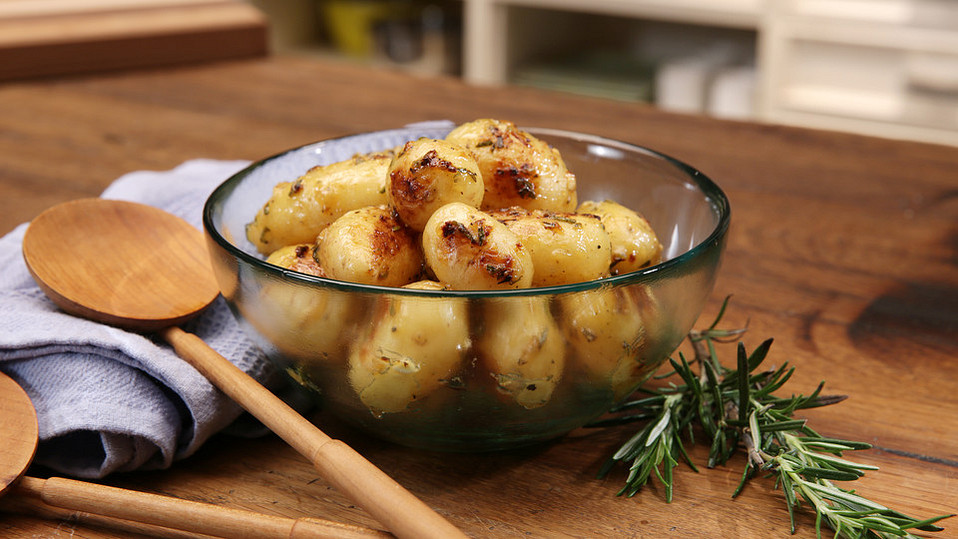
\includegraphics[width=.9\linewidth]{pics/Schwenkkartoffeln}
		\captionof{figure}{Schwenkkartoffeln von der Plancha}
		\label{fig:Schwenkkartoffeln}
	\end{minipage}
\end{figure}
\newpage

\subsection{Süßkartoffeln oder Kartoffeln aus der Folie}

\paragraph{Geräte}

\begin{itemize}[noitemsep]
	\item Kugelgrill oder Keramikgrill
\end{itemize}

\paragraph{Zutaten}
	
\begin{itemize}[noitemsep]
	\item Süßkartoffeln oder mehlig kochende Kartoffeln je nach Bedarf
\end{itemize}

\paragraph{Zubereitung}

Die Süßkartoffeln/ Kartoffeln in erst Backpapier und dann in Alu-Folie 
einwickeln.
Die Süßkartoffeln für ca. 45 Minuten die mehlig kochenden Kartoffeln evtl. kürzer 
direkt in die Glut legen. Nach 45 Minuten auspacken und servieren siehe 
Abbildungen~\vref{fig:Suess} ~\vref{fig:Folienkartoffel} Dazu wird ein Dip je nach Bedarf 
gereicht.
\newpage

\begin{figure}[htbp]
	\centering
	\begin{minipage}{1\textwidth}
		\centering
		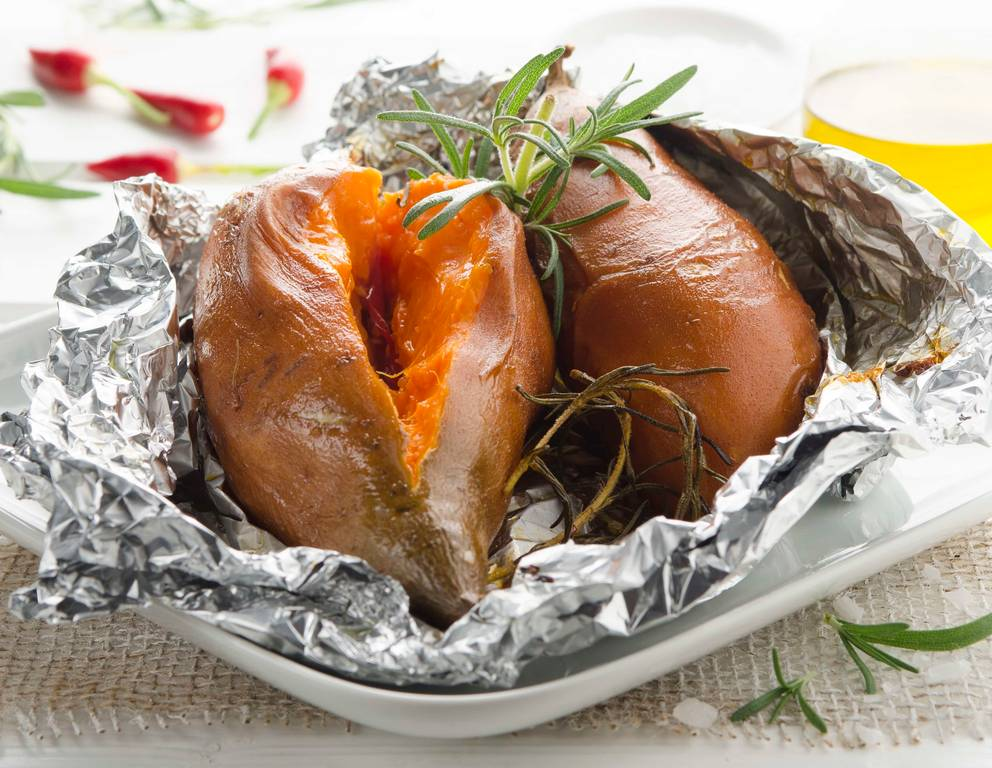
\includegraphics[width=.9\linewidth]{pics/Suess}
		\captionof{figure}{Foliensüßkartoffel vom Grill}
		\label{fig:Suess}
	\end{minipage}
\end{figure}

\begin{figure}[htbp]
	\centering
	\begin{minipage}{1\textwidth}
		\centering
		\includegraphics[width=1\linewidth]{pics/Folienkartoffel}
		\captionof{figure}{Folienkartoffel vom Grill}
		\label{fig:Folienkartoffel}
	\end{minipage}
\end{figure}
\newpage

%Beilagen
%!TEX root = Vorlage_Buch.tex
\chapter{Salate, Salate und noch mehr Salate}\label{Chapter6}
\lettrine[lines=3]{S}{alate sind die Vitaminbomben} des BBQ's, sind  Vorspeisen, Sättigungsbeilagen, Desserts oder einfach nur lecker. Da 
Salate für das BBQ
unentbehrlich sind, zumindest bei mir ist es so, habe ich auch Salate in dieses Buch aufgenommen. 

Salate werden in mannigfaltigen Versionen und Geschmacksrichtungen bei jedem kulinarischen Event präsentiert. Ich liebe leichte Salate 
die mich nicht von
den anderen Köstlichkeiten des BBQ's ablenken und gerade deshalb alles abrunden.

Im Weiteren werden wir Vorspeise- oder Beilagensalate, Salate als Sättigungsbeilagen und Desserts kennenlernen. 

\section{ Vorspeisen und Beilagensalate}

\subsection{Klassischer Kopfsalat}

Der klassische Kopfsalat darf eigentlich nirgends fehlen. Es ist ein einfacher Salat den jeder kennt. Er wird gerne als Vorspeise- oder 
Beilagensalat serviert, siehe Abbildung~\vref{fig:Kopfsalat}. 


\paragraph{Für den Salat}

\begin{itemize}[noitemsep]
	\item 1 Kopf Kopfsalat
\end{itemize}

Optionale Zutaten

\begin{itemize}[noitemsep]
	\item Keimlinge (Linsen, Mungobohne, Kicherbsen u.v.m. )
	\item Scheiben von Radieschen
	\item Julienne von Karotten
	\item und Weiteres mehr, je nach Geschmack
\end{itemize}


\paragraph{Für die Vinaigrette}

\begin{itemize}[noitemsep]	
	\item 1 kleine Zwiebel  (oder Charlotte oder rote Zwiebel, je nach Geschmack)
	\item 3 EL Pflanzenöl (oder Raps- oder Sonnenblumenöl)
	\item 1 EL Essig (ich verwende Altmeister von Hengstenberg)
	\item 1 TL Delikatesssenf
	\item 1 Spritzer Flüssigwürze (hier Maggi Würze)
	\item Salz 
	\item Zucker (soviel wie Salz)
	\item Pfeffer
	\item Kräuter nach Geschmack (hier Schnittlauch und Petersilie)
	
	\item 1/2 EL Wasser
\end{itemize}

\paragraph{Zubereitung}

Den Kopfsalat waschen und rupfen. Bitte nicht mit den Messer schneiden, da der Salat sonst rostig wird. In kaltem Wasser waschen und 
abtropfen lassen, evtl. 
schleudern.
Tipp: Ist der Salat aus dem eigenen Garten kann er in Salzwasser gewaschen werden, so entfernt man die tierischen Bewohner. Ist der 
Salat ein wenig welk in 
lauwarmen 
Wasser waschen, so bekommt er die Knackigkeit zurück, alternativ kann der Salat auch für längere Zeit (ca. 20 Minuten) in kaltem 
Wasser liegen.

Zur Zubereitung der Vinaigrette, Öl, Essig, Senf und Maggi in die Salatschüssel geben und mit dem Salatbesteck rühren bis eine 
homogene Flüssigkeit entsteht. 
Für die 
Verbindung zwischen Öl und Essig sorgt der Senf. Die Zwiebeln, Salz, Zucker, Pfeffer und die Kräuter zugeben. Ein wenig Wasser öffnet 
die Vinaigrette. Den 
trockenen 
Kopfsalat zugeben und kurz vor dem Servieren durchmischen und die Keimlinge darüber streuen.
\newpage
\begin{figure}[h]
	\centering
	\includegraphics[scale=.4]{pics/Kopfsalat}
	\caption{Kopfsalat}
	\label{fig:Kopfsalat}
\end{figure}

\subsection{Feldsalat mit Speck und Croutons}
Der Feldsalat wird gerne als Salat im Winter gereicht, daher ist der Salat als Vorspeise für ein Grillabend im Winter perfekt geeignet, siehe 
Abbildung~\vref{fig:Feldsalat}.

\paragraph{Für den Salat}

\begin{itemize}[noitemsep]
	\item 500 g Feldsalat
\end{itemize}	

\paragraph{Für die Vinaigrette}

\begin{itemize}[noitemsep]	
	\item 1 kleine Zwiebel  (oder Charlotte oder rote Zwiebel, je nach Geschmack)
	\item 3 EL Pflanzenöl (oder Raps- oder Sonnenblumenöl)
	\item 1 EL Essig (ich verwende Himbeeressig)
	\item 1 TL Delikatesssenf
	\item 1 Spritzer Flüssigwürze (hier Maggi Würze)
	\item Salz 
	\item Zucker (soviel wie Salz)
	\item 1/2 EL Wasser
	\item Croutons
	\item angebratener Schinkenspeck
\end{itemize}

\begin{figure}[h]
	\centering
	\includegraphics[scale=.35]{pics/Feldsalat}
	\caption{Feldsalat mit Speck und Croutons}
	\label{fig:Feldsalat}
\end{figure}

\paragraph{Zubereitung}

Den Feldsalat waschen und ausputzen. Danach mit der Vinaigrette anmachen, auf dem Salatteller anrichten
und je nach Geschmack mit Croutons und dem Speck bestreuen.  

\subsection{Wintersalat mit Orangen und Ziegenkäse}
Auch dieser Salat ist mit seiner Aromatik von Südfrüchten, dem tollen Geschmack von Feldsalat und dem herben Einfluss des Radiccio
auch als Vorspeise beim Wintergrillen eine sehr gute Wahl.

\paragraph{Für den Salat}

\begin{itemize}[noitemsep]
	\item 1 halber mittelgroßer Kopf Radiccio
	\item 1 handvoll Feldsalat
	\item 1 gr. Gelbe Beete (optional Rote Beete)
	\item 1 handvoll Nüsse und Kerne (z.B. Pekanüsse und Kürbiskerne)
	\item 2 Orangen
	\item 1 halbe Avocado
	\item 6 Scheiben Ziegenkäse von der Rolle (oder Feta)
\end{itemize}	

\paragraph{Für das Dressing}

\begin{itemize}[noitemsep]
	\item Etwas Saft der filetierten Orangen
	\item 2 EL Balsamicocreme
	\item 1 EL Traubenkernöl (oder Olivenöl)
	\item 1 TL Honig
	\item  Salz
\end{itemize}

\paragraph{Zubereitung}

Die Gelbe Beete schälen in Würfel schneiden und auf einem mit Backpapier 
ausgelegtem Backblech verteilen. Mit etwas Olivenöl beträufeln und 
mit Salz würzen. Im vorgeheizten Ofen ca. 20 Minuten backen. Aus dem Ofen 
holen und etwas abkühlen lassen. In der Zwischenzeit den Radicchio
in kleine Stücke zupfen, in handwarmem Wasser waschen. Den Feldsalat 
putzen und in kaltem Wasser waschen. Beide Salate in einem Sieb gut
abtropfen lassen oder in einer Salatschleuder trockenschleudern. Die Orangen 
schälen und in Scheiben schneiden. Dabei versuchen, möglich etwas
Saft für das Dressing aufzufangen. Die Avocado schälen und in Stücke 
schneiden. Die Nüsse und Kerne nach Bedarf in einer Pfanne ohne Fett kurz 
rösten .

Für das Dressing alle Zutaten gut miteinander verrühren. Den Salat mit der 
Avocado, der Gelben Beete und den Orangen auf einer Platte anrichten. 
Die Nüsse darüber streuen. Kurz vor dem Servieren die Ziegenkäsescheiben in 
einer Pfanne ohne Fett auf geringer Stufe etwas schmelzen lassen. 
Aus der Pfanne nehmen und auf dem Salat anrichten. Mit dem Dressing 
beträufeln und sofort servieren, siehe \vref{fig:Wintersalat}.

\begin{figure}[htbp]
	\centering
	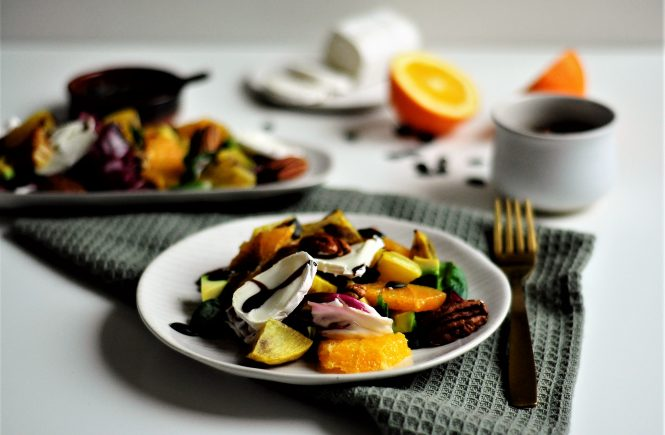
\includegraphics[scale=.6]{pics/Wintersalat}
	\caption{Ein köstlicher Wintersalat}
	\label{fig:Wintersalat}
\end{figure}
\newpage
\subsection{Gegrillter Butternusskürbis-Salat}
Kürbisse eignen sich hervorragend zum Grillen. Als Beilage zum zu gegrillten 
Fisch, Rind und Schwein eignet dieser Salat aus gegrillten Butternusskürbis 
super.

\paragraph{Für den Salat}

\begin{itemize}[noitemsep]
	\item 1 Butternusskürbis (ca. 800g)
	\item 6 EL Olivenöl
	\item 1 Dose (425 g) Kichererbsen
	\item 120 g Blattspinat
	\item 12 Kirschtomaten
	\item 3 Lauchzwiebeln
	\item 1 kleine Salatgurke (ca. 250 g)
	\item 50 g Haselnusskerne
	\item 3 EL Essig (bei mir Altmeister von Hengstenberg)
\end{itemize}

\begin{figure}[htbp]
	\centering
	\includegraphics[scale=.35]{pics/Kürbis1}
	\caption{Gegrillter Butternusskürbis-Salat}
	\label{fig:Kürbis1}
\end{figure}

\paragraph{Zubereitung}

Die Holzspieße in Wasser einweichen. Den Kürbis putzen, längs halbieren und 
das Kerngehäuse entfernen. Das Fruchtfleisch in walnussgroße Stücke 
schneiden
und in reichlich kochendem Salzwasser ca. 6 Minuten kochen. Die gekochten 
Kürbisstücke abgießen und unter fließendem kalten Wasser abkühlen. Die 
Kürbisstücke gut abtropfen lassen und mit 3 EL Olivenöl in eine Schüssel 
mischen. Danach mit Salz und Pfeffer würzen.

Kürbis auf Holzspieße stecken. In einer Grillschale auf dem heißen Grill 6–8 
Minuten unter Wenden grillen. Holzspieße vom Grill nehmen. Kürbisstücke von 
den 
Spießen in eine Schüssel streifen.

Kichererbsen in einem Sieb gut abtropfen lassen. Blattspinat putzen, waschen 
und trocken schleudern. Tomaten waschen und halbieren. Lauchzwiebeln 
waschen,
trocken schütteln und in Ringe schneiden. Gurke putzen, waschen und in 
Würfel schneiden.

Kichererbsen, Spinat, Tomaten, Lauchzwiebeln, Gurke, Haselnüsse, Essig und 
restliches Öl zum Kürbis geben und vorsichtig untermischen. Mit Salz und 
Pfeffer
abschmecken und anrichten, siehe \vref{fig:Kürbis1}.

\section{Weiter geht es mit den Beilagensalaten}

\subsection{Coleslaw}\label{Coleslaw}

Coleslaw ist ein amerikanischer Krautsalat, der hauptsächlich aus fein 
geschnittenem Weißkohl und Möhren besteht. Was diesen Salat besonders 
macht, ist das cremige Dressing,

Der Coleslaw wird oft als Beilage zu BBQ-Gerichten, Sandwiches oder Burgern 
serviert und ist bekannt für seine erfrischende und gleichzeitig reichhaltige 
Textur. Die Kombination aus knackigem Gemüse und dem cremigen Dressing 
macht ihn zu einem beliebten Gericht bei vielen Gelegenheiten.

\paragraph{Für den Coleslaw}

\begin{itemize}[noitemsep]
	\item 1 Weißkohl (ca. 1,4 kg)
	\item 1 Karotte
	\item 1 Zwiebel, klein
	\item 200g Mayonnaise
	\item 80 g Sahne
	\item 2 EL Weinessig
	\item 4 EL Zucker
	\item 1 TL Selleriesamen
	\item Himalaya-Salz
	\item Schwarzer Pfeffer
\end{itemize}

\paragraph{Zubereitung}

Der Weißkohl wird halbiert, der Strunk entfernt und der Kohl feine Streifen 
geschnitten. Zusammen mit der fein geraspelten Karotte und der fein 
geschnittenen Zwiebel wird der Weißkohl vermischt.

Für die Sauce werden die Mayonnaise, Sahne, Weinessig, Zitronensaft, Zucker 
und Selleriesamen vermischt und mit Salz und Pfeffer abgeschmeckt. Die 
Selleriesamen sollten zuvor im Mörser zerstoßen werden, damit sich das Aroma 
besser entfalten kann. Die fertige Sauce über den Coleslaw geben und gut 
einmassieren. Das ganze über Nach im Kühlschrank durchziehen lassen. Vor 
dem Servieren nachmals gut durchrühren, siehe \vref{fig:Coleslaw}.

\begin{figure}[htbp]
	\centering
	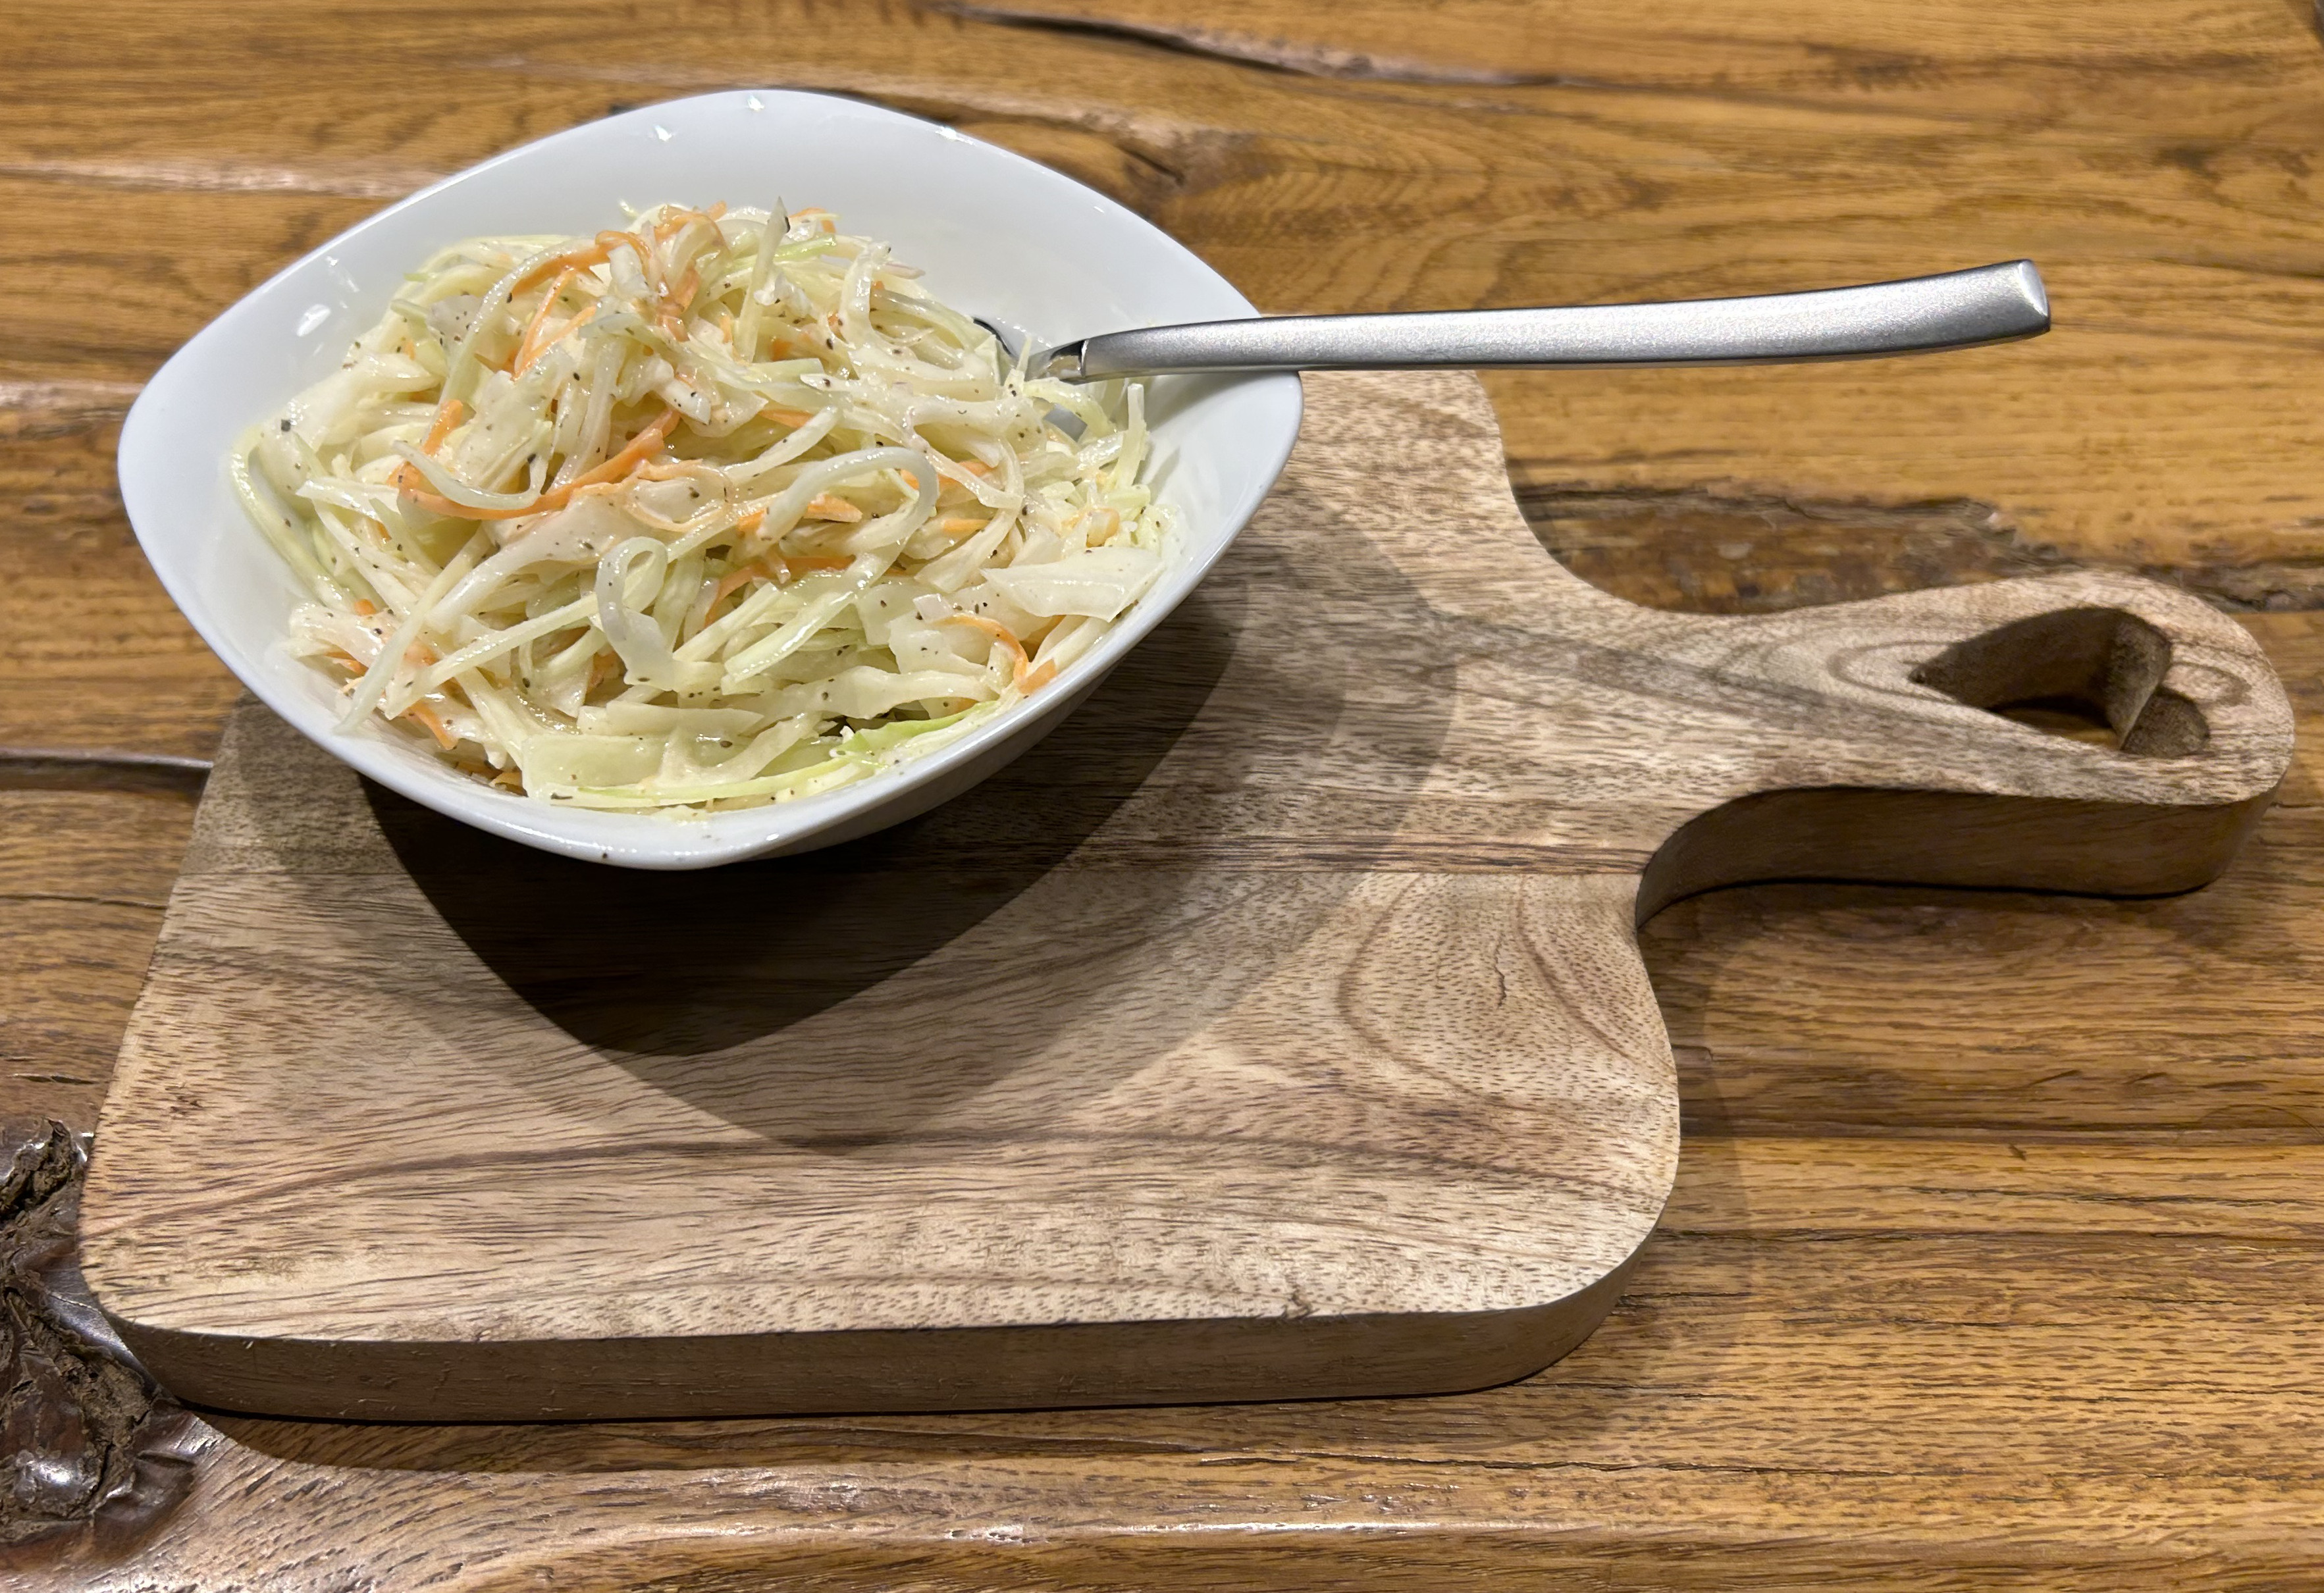
\includegraphics[scale=.4]{pics/Coleslaw}
	\caption{Amerikanischer Krautsalat, sehr gut passend zu BBQ}
	\label{fig:Coleslaw}
\end{figure}

\subsection{Feldsalat mit Mozzarella und Tomatendressing}

\paragraph{Für den Salat}

\begin{itemize}[noitemsep]
	\item 1 L Tomatensaft
	\item 1 Zwiebel
	\item 1 Knoblauchzehe
	\item 2 EL Zucker
	\item 150 ml Balsamico oder Apfelessig
	\item 4 Kugeln Mozzarella
	\item 500g Feldsalat
	\item 200g Bacon
	\item 2 Tomaten
\end{itemize}

\paragraph{Zubereitung}

Die Zwiebel und  Knoblauchzehe fein schneiden. In Olivenöl anschwitzen.
Den Zucker zugeben und leicht karamellisieren. Mit dem Essig ablöschen und 
reduzieren.
Tomatensaft hinzugeben,  auf 1/3 der Menge reduzieren und von der Flamme 
nehmen. 
Die Tomaten entkernen und in Würfel schneiden

Die Mozzarellakugel in der Mitte des Tellers platzieren Tomatendressing leicht 
aufwärmen und rund
um die Mozzarellakugel verteilen.  Den Feldsalat auf dem Dressing drapieren 
die Tomaten darauf verteilen 
und alles mit Olivenöl beträufeln. Die angebratenen Baconscheiben halbieren 
und auf den Feldsalat legen. 
Die Mozzarellakugel kreuzförmig einschneiden und mit dem angewärmten 
Tomatendressing übergießen. 
Den Salat servieren.

\subsection{Eisbergsalat mit Champignons und Tomatendressing}

\paragraph{Für den Salat}

\begin{itemize}[noitemsep]
	\item 1 Eisbergsalat
	\item 1 Schale Champignons
	\item Olivenöl
	\item 1 Zehe Knoblauch
\end{itemize}

Zutaten für das Dressing:
\begin{itemize}[noitemsep]
	\item 1l Tomatensaft
	\item 1 kleine Zwiebel
	\item 1 Knoblauchzehe
	\item 150 Essig Balsamico oder Apfelessig
	\item 2 EL Zucker
	\item 1 Tomate
\end{itemize}

\paragraph{Zubereitung}

Die Zwiebel und  Knoblauchzehe fein schneiden. In Olivenöl anschschwitzen.
Den Zucker zugeben und leicht karamellisieren. Mit dem Essig ablöschen und 
reduzieren.
Tomatensaft hinzugeben,  auf 1/3 der Menge reduzieren und von der Flamme 
nehmen. 
Die Tomaten entkernen und in Würfel schneiden.

Die Champignons in Scheiben,  die Tomate entkernen und in Würfel schneiden. 
Die Champignons mit dem Knoblauch in 
Olivenöl anbraten. Dressing auf den Salattellern verteilen. Den Eisbergsalat, 
trocknen und auf dem Dressing verteilen. Den 
Salat mit den Champignons und Tomatenwürfeln anrichten und servieren.
% Salate
%!TEX root = Vorlage_Buch.tex
\chapter{Gewürze, Saucen und Dips}\label{Chapter7}
\lettrine[lines=3]{G}{ewürze} und Kräuter sind aus der Küche nicht 
wegzudenken. 
Gewürze und Kräuter werden eingesetzt um die Geschmacksvielfalt 
verschiedener Regionen
und deren Fusionen widerzuspiegeln.
Sie wirken konservierend, sind gesundheitsfördernd und steigern das 
Wohlbefinden.
Sie enthalten Säuren, Zucker, ätherische Öl und andere Komponenten die 
einzigartig in
Geschmack und Wirkung sind. Das bilden verschiedener Komplexe durch 
chemische 
Reaktionen mit dem Grillgut führen Veränderungen der Textur, entwickeln 
Aromen und konservieren.
   

\section{Gewürze und Gewürzmischungen}
Die Mischungen die aus verschiedenen Gewürzen zusammengesetzt sind, sind 
zum Teil bestens gehütete Geheimnisse. Gewürzmischungen  sind unter anderem 
Alleinstellungsmerkmale
in der professionellen Küche und dem Gewürzhandel. Vor allen im Orient findet 
man eine schier
unendliche Zahl vom Familienrezepten verschiedener Gewürzmischungen. In 
der kreolischen Küche  stellt sich nicht anders dar.
In der deutschen Küche haben die Gewürze ebenfalls Einzug gehalten, das ist 
vor allem in der Grillszene und der Gastronomie zu verdanken.

\subsection{Kansas City Rib Rub}\label{Kansas}
Kansas City ist die Welthauptstadt des Barbecue, in der die jährliche 
Grillweltmeisterschaft, der größte Grillwettbewerb  der Welt,  veranstaltet wird. 
Es ist daher nicht verwunderlich, dass es auch Rubs gibt die nach Kansas City 
benannt wurden. Hier ist ein Rub der perfekt zu Schweinefleisch passt, da in 
Kansas City vor allen Rippchen serviert werden.
\paragraph{Für den Rub}

\begin{itemize}[noitemsep]
	\item 8 EL brauner Zucker
	\item 4 EL Paprikapulver
	\item 1 EL Salz
	\item 1 EL schwarzer Pfeffer, ganze Körner
	\item 1 EL Zwiebelpulver
	\item 1 EL Knoblauchpulver
	\item 1 TL Cayennepfeffer
	\item 1 TL Chilipulver
\end{itemize}

\paragraph{Zubereitung}

Um das Aroma dieses Rubs zu vertiefen röste ich den Schwarzen Pfeffer in der 
Pfanne an, bis 
knackende Geräusche entstehen. Nach dem Rösten wird der Pfeffer im Mörser 
zerkleinert. Die Zutaten mischen, fertig.

\subsection{Magic Dust}\label{Magic}

">Magic Dust"< ist ein vielseitiger Rub  und aus der Grillszene nicht weg zu 
denken. Durch die Kombination aus rauchigen, würzigen und süßen Noten ist 
er universell einsetzbar und passt zu fast allem das man grillen kann. Diese 
Mischung bringt durch ihre Kombination der Aromen und würzigen Noten den 
perfekten Geschmack auf Fleisch und andere Speisen. Typische Zutaten sind 
Paprika, brauner Zucker, Salz, Knoblauch- und Zwiebelpulver, Senfpulver, 
Chilipulver und manchmal ein Hauch Cayennepfeffer für zusätzliche Schärfe.

\paragraph{Für den Rub}

\begin{itemize}[noitemsep]
	\item 3 EL Paprikapulver, edelsüß
	\item 2 EL grobes Meersalz
	\item 2 EL brauner Zucker
	\item 2 EL Chilipulver Zucker
	\item 1 EL geräuchertes Paprikapulver
	\item 1 EL Senfpulver
	\item 1 EL Knoblauchpulver
	\item 1 EL Zwiebelpulver
	\item 1 TL Cyannepfeffer
\end{itemize}

\paragraph{Zubereitung}

Um das Aroma dieses Rubs zu vertiefen röste ich den Schwarzen Pfeffer in der 
Pfanne an, bis 
knackende Geräusche entstehen. Nach dem Rösten wird der Pfeffer im Mörser 
zerkleinert. Die Zutaten mischen, fertig.

\subsection{Chicken Rub}\label{Chicken}
Das Chicken Rub ist das perfekte Rub für Hähnchen. Ob Drumsticks, komplette 
Keulen oder das Road Killed Chicken. Mit diesem leicht herzustellenden Rub 
haben wir ein universelles Hähnchengewürz mit Geschmacksgarantie.

\begin{itemize}[noitemsep]
	\item 5 EL Paprikapulver, edelsüß
	\item 3 EL Salz
	\item 2 EL schwarzer Pfeffer, frisch gemahlen
	\item 2 EL Zwiebelpulver
	\item 2 EL Knoblauchpulver
	\item 1 EL Oregano, getrocknet
	\item 1 EL Thymian, getrocknet
	\item 1 EL Cayennepfeffer
\end{itemize}

\paragraph{Zubereitung}

Die Zutaten mischen, fertig.

\subsection{Bratkartoffelgewürz}

\paragraph{Für das Bratkartoffelgewürz}\label{Bratkartoffelgewürz}

\begin{itemize}[noitemsep]
	\item 50 g Meersalz
	\item 20 g Bockshornklee
	\item 1/2 TL Koriandersaat, gemahlen
	\item 1/2 TL  Knoblauchpulver
	\item 1/2 TL  Paprika, edelsüß
	\item 1/2 TL Zwiebelpulver
	\item 1 Prise geräucherter Paprika
	\item 1 Prise Muskatnuss, frisch gerieben
	\item 1 Prise Fenchelsaat, gemahlen
	\item 1 Prise Cumin, gemahlen
	\item 1/2 TL Kaschmir-Chili-Pulver
	\item 1 Prise Schwarzer Pfeffer, gemahlen
	\item 1 kleine Prise Nelken, gemahlen
\end{itemize}

\paragraph{Zubereitung}

Die Zutaten mischen, fertig.

\subsection{Gewürzmischung für das Schwarze Chili}\label{Gewürzmischung}

\paragraph{Zutaten}

\begin{itemize}[noitemsep]
	\item 1 EL gekörnte Brühe
	\item 3 TL Chilipulver (aus eigener Herstellung, das hat richtig Dampf)
	\item 20 g Zartbitterschokolade (hier 70\% Kakaoanteil)
	\item 1 TL Kümmelpulver
	\item 1 gestr. TL Oregano
	\item 1 gestr. TL Koriander
	\item 1 gestr. TL Estragon
	\item 1/2 TL Kleiner Langpfeffer (ist der kleine Bruder des Bengal-Pfeffers, Bezugsquelle \url{www.gewuerzshop-mayer.de})
	\item 1/2 TL Zimt (gibt dem ganzen eine festliche Note)
	\item 2 EL Ras el Hanut ("`Chef der Küche"' der macht die ganze Sache Rund)
\end{itemize}

\paragraph{Zubereitung}

Die Zartbitterschokolade in eine Schüssle reiben, die restlichen Zutaten 
hinzufügen, gut durchmischen, fertig. Soll das Gewürz in größeren Mengen auf 
Vorrat hergestellt werden, kann die Zartbitterschokolade durch Kakaopulver 
ersetzt werden. In diesem Falle nur 2/3 des  Gewichtanteils verwenden.

\section{Öle und Soßen}
{Vom Arganöl bis zur Zitronenmayo}

\subsection{Chiliöl-mit-Crunch}
{Knuspriges Chili-Öl}
hört widersprüchlich an,  es gibt aber tatsächlich ein Rezept für Chili-Öl mit 
knusprigen Zutaten. Das für den universellen Einsatz wie geschaffen ist. Ich 
empfehle je nach Leidensfähigkeit das Öl in verschiedenen Schärfestufen 
herzustellen. Um ein schokoladiges Dessert zu verfeinern ist es nicht förderlich 
ein höllisch scharfes Chili-Öl zu verwenden. Während zum verfeinern einer 
Pizza oder Spareribs schon ein Öl mit etwas mehr Dampf benutzt werden kann.

Das Grundrezept kommt mit wenigen Zutaten aus und liefert bereits ein 
Hammerergebnis.
Ich stelle euch außerdem einige Ideen vor um das Rezept für den eigenen 
Geschmack anzupassen.
\newline

\paragraph{Für das Grundrezepts:}

\begin{itemize}[noitemsep]
	\item 1 Liter neutrales Speiseöl, etwa Raps
	\item 90 g getrocknete Chilis oder Chiliflocken,  je nach Vorliebe auch mehr
	\item 5-8 Schalotten
	\item 1/2 Knolle Knoblauch
	\item 50 ml Sojasoße
	\item 20 g Zucker (ich nehme gerne Rohrzucker, der süßt nicht so stark wie 
	Rübenzucker, das kann nach belieben ausgeglichen werden) 
\end{itemize}

\paragraph{Optional:}

\begin{itemize}[noitemsep]
	\item 50 ml Balsamico Essig
	\item Gewürze wie Zimt,  Ingwer,  Anis
	\item 100 g Sesam oder gehackte Erdnüsse/ Cashewkerne
\end{itemize}

\paragraph{Zubereitung}

Das Öl in einem großen Kochtopf auf mittlere Hitze bringen und die Gewürze 
wie Zimt,  Anis und Ingwer darin für etwa 10 Minuten frittieren, um das Öl zu 
aromatisieren. Die Gewürze anschließend mit einer Schöpfkelle aus dem Öl 
fischen und entsorgen.
Die Schalotten und den Knoblauch schälen und in möglichst feine Scheiben 
schneiden. Wer einen feinen Hobel oder eine Mandoline hat, nimmt sie zu Hilfe. 

Die Schalotten brauchen deutlich länger als der Knoblauch. Schalotten sind 
nach 10 bis 15 Minuten fertig, Knoblauch schon nach ein bis zwei Minuten. Gibt 
man beide gleichzeitig rein, verbrennt Letzterer nur. Daher: Schalotten und 
Knoblauch nacheinander im aromatisierten Öl knusprig braun frittieren lassen. 
Wenn die Blubberblasen deutlich nachlassen, ist die meiste Flüssigkeit aus 
dem Gemüse verschwunden, und wir haben ein Maximum an Crunch erreicht – 
danach kommt nur noch Asche. Also fix mit der Schöpfkelle herausnehmen und 
beiseite legen.
Die Chiliflocken und das knusprige Element wie Sesam oder Nüsse in eine 
hitzefeste Schale oder einen Topf legen, dann das heiße Öl obendrauf gießen. 
Niemals direkt in ein Glas gießen, dieses könnte springen! Das Öl ist noch lange 
heißer, als es aussieht.
Alles gut abkühlen lassen (etwa 30 bis 45 Minuten) und dann mit Zucker, 
Sojasoße und Essig abschmecken. Vorsicht: Wenn das Öl noch zu heiß ist, 
blubbert es bei der Zugabe von Essig und anderen Flüssigkeiten. Also lieber 
warten.
Die knusprigen Schalotten und den Knoblauch unterrühren und alles mit einer 
Kelle in sterile Gläser umfüllen, etwa abgekochte Marmeladengläser.
\paragraph{Variationen} Wer sich austoben möchte, kann gerade bei diesem 
Rezept sehr viel ausprobieren. Ein paar Ideen:

Zunächst gibt es eine riesige Varianz an Chilisorten, von mittel- und 
südamerikanischen hin zu asiatischen. Chipotles (geräucherte Jalapeños) 
bringen etwa einen tollen Rauchgeschmack mit rein. Thailändische Bird’s Eye 
Chilis sind scharf wie die Hölle, koreanisches Gochugaru hingegen oft 
vergleichsweise mild. Auch frische Chilis können verwendet werden, dann sinkt 
aber die Haltbarkeit.
Für mehr Tiefe und Herzhaftigkeit kann man auch getrocknetes Pilzpulver 
hinzugeben oder etwas Würzsoße mit Glutamat.

Wer etwa Fünf-Gewürze-Pulver oder weißen Pfeffer hinzufügt, macht dies am 
besten erst, wenn das Öl weit genug abgekühlt ist, um in Gläser umgefüllt zu 
werden. Dasselbe gilt für andere Pulvergewürze.
Szechuanpfeffer, Curryblätter oder Kaffirlimettenblätter können dem Öl weitere 
leckere Aromen hinzufügen.
Wer mag, kann das Öl oder Anteile davon ersetzen. Sesamöl etwa hat ein tolles 
Aroma, sollte jedoch nicht zu stark erhitzt werden (sonst geht ebenjenes 
Aroma flöten). Sesamöl also erst zum Verfeinern am Ende des Prozesses mit 
ins Glas geben. Soja- oder Erdnussöl bringen viel Eigengeschmack mit und 
können von Anfang an verwendet werden – kosten aber auch mehr als Rapsöl.
Man kann die Menge der knusprigen Einlage deutlich nach oben skalieren. 
Gerade geröstete und gehackte Erdnüsse sind günstig zu bekommen.

\paragraph{Zutaten für die Orangen-Chili-Butter}

\begin{itemize}[noitemsep]
	\item 4 EL Geklärte Butter
	\item 1 Rote Chilischote (Cayenne)
	\item 1/2 Bio-Orange
	\item 1 TL Fenchelsamen
\end{itemize}

\paragraph{Zubereitung}

Die Butter erhitzen. Die Chilischote entkernen und in sehr feine Ringe schneiden 
und zusammen 
mit dem Fenchelsamen in der Butter bei 
schwacher Hitze 1 bis 2 Minuten garen. In der Zwischen Zeit mit einem 
Sparschäler von der 
gewaschenen Orange die Hälfte der Schale 
abschälen und in sehr feine Streifen schneiden. Die Orangenstreifen unter die 
Butter mischen 
und alles auf einem Reschaud warmhalten.

\subsection{Orangen-Chile-Butter}

Die Orangen-Chili-Butter ist eins schnelle Topping für Pasta, Baguette oder 
Geflügel. Das 
einfache Rezepte hat eine fantastische 
Aromatik, eine milde Säure und eine dezente Schärfe.

\paragraph{Zutaten für die Orangen-Chili-Butter}\label{OrangenChili}

\begin{itemize}[noitemsep]
	\item 4 EL Geklärte Butter
	\item 1 Rote Chilischote (Cayenne)
	\item 1/2 Bio-Orange
	\item 1 TL Fenchelsamen
\end{itemize}

\paragraph{Zubereitung}

Die Butter erhitzen. Die Chilischote entkernen und in sehr feine Ringe schneiden 
und zusammen 
mit dem Fenchelsamen in der Butter bei 
schwacher Hitze 1 bis 2 Minuten garen. In der Zwischen Zeit mit einem Sparschäler von der 
gewaschenen Orange die Hälfte der Schale 
abschälen und in sehr feine Streifen schneiden. Die Orangenstreifen unter die Butter mischen 
und alles auf einem Reschaud warmhalten.

\subsection{Ketchup}
Ketchup ist beim Grillen nicht wegzudenken. Pur oder als Basis für andere 
Saucen. Ein gutes Ketchup ist ein muss für jeden BBQ-Fan.
Ich habe hier ein Rezept zusammengestellt, das nicht nur super schmeckt 
sondern auch leicht nachzukochen ist. 
\newline

\paragraph{Grundrezept für das Ketchup}\label{Ketchup}

\begin{itemize}[noitemsep]
	\item 1,5 kg Tomaten (am Besten Flaschentomaten)
	\item 1 Zwiebel
	\item 1 Zehe Knoblauch
	\item 100 g Brauner Zucker
	\item 80 ml Essig (mild, z.B. Rotweinessig oder Apfelessig)
	\item 2 Gewürznelken
	\item 2 Lorbeerblätter
	\item 1/4 TL Five Spices
	\item TL Salz
	\item 1 EL Öl
\end{itemize}

\paragraph{Zubereitung}

Zwiebel und Knoblauch hacken. Die Tomaten waschen, häuten und in Stücke 
schneiden.

Öl in einem Topf erhitzen, Zwiebeln und Knoblauch darin langsam dünsten, bis 
sie glasig sind.
Dann die kleingeschnittenen Tomaten und die Gewürze (außer Essig und 
Zucker) zugeben. Unter gelegentlichem
Rühren ca. 30 Minuten köcheln lassen.

Jetzt Zucker und Essig zugeben, unterrühren, einmal aufkochen. Dann kannst 
Du den selbstgemachten 
Ketchup final abschmecken und noch warm in die Gläser abfüllen. Die Gläser 
dann sofort fest verschießen.

\subsection{Habanero BBQ Sauce}
Wer nicht gerne scharf isst, sollte diese Rezept auf keinem Fall ausprobieren, 
denn diese Sauce hat es in sich. Habaneros sind bekannt für ihre feurige 
Schärfe, aber auch für ihren fruchtigen Geschmack. Beides kommt in dieser 
Sauce perfekt zur Geltung.
\newline

\paragraph{Für die Habanero BBQ Sauce}

\begin{itemize}[noitemsep]
	\item 1 Tube Tomatenmark à 200 ml (dreifach konzentriert)
	\item 4 Habaneros, frisch
	\item 1 Zwiebel
	\item 120 ml Apfelessig
	\item 120 ml Wasser
	\item 30 g Senf (je nach Geschmack)
	\item 2 EL Sojasauce
	\item 1 TL Paprikapulver (geräuchert)
	\item Salz
	\item Pfeffer
\end{itemize}

\paragraph{Zubereitung}

Die Habanero BBQ Sauce ist schnell zubereitet und benötigt nicht viele Zutaten.
\textbf{Wichtig:} \emph{Ziehe beim Schneiden der Habaneros Handschuhe an, 
	denn brennen sollen die 
	scharfen Chilischoten nur beim Essen, nicht bei der Zubereitung.} Wenn du 
	die Habaneros etwas 
„entschärfen“ möchtest, entferne die Kerne teilweise oder komplett.

Sie sieht zwar nicht so aus, aber die Habanero BBQ Sauce ist unglaublich sc
harf und lecker zugleich.

Die Zwiebel fein würfeln. Habaneros in feine Stücke schneiden (Handschuhe 
anziehen).
Die Zwiebelwürfel in etwas Öl glasig dünsten. Dann die Habaneros und alle 
anderen Zutaten 
hinzugeben und verrühren.
Alles etwa eine halbe Stunde köcheln lassen.
Das Rezept sieht vier Habanero-Schoten vor, du kannst die Menge und damit 
den Schärfegrad aber 
ganz nach deinen Wünschen variieren.

\subsection{Klassische amerikanische BBQ-Sauce}
Diese Sauce sollte bei keinem BBQ fehlen. Der Klassiker unter den BBQ Saucen 
ist ein absoluter Allrounder und passt zu ziemlich jedem Grillgut.
Am besten schmeckt sie natürlich, wenn du die selber machst.

Tomaten sorgen für einen fruchtigen Geschmack, brauner Zucker für die Süße, 
Essig für die Säure und Chili für eine angenehme Schärfe. Das
sind die wichtigsten Grundzutaten für die klassisch amerikanische BBQ Sauce.
\newline

\paragraph{Für die BBQ Sauce}

\begin{itemize}[noitemsep]
	\item 200 ml Tomaten passiert
	\item 100 ml Ketchup (Rezept \vref{Ketchup})
	\item 50 ml Rotweinessig
	\item 50 g Brauner Zucker
	\item 1 Zwiebel
	\item 2 Zehen Knoblauch
	\item 50 ml Wasser
	\item 1 TL Paprikapulver
	\item 1/2 Chiliflocken
	\item 1/2 Senf
	\item 1/2 Salz
\end{itemize}

\paragraph{Zubereitung}

Knoblauch und Zwiebeln fein würfeln und glasig dünsten.

Dann alle weiteren Zutaten zugeben und etwa eine halbe Stunde köcheln 
lassen, bis die gewünschte Konsistenz erreicht ist. Fertig.

\subsection{Salsa de las albóndigas}\label{SalsaAlbondigas}

Die Salsa de las Albóndigas wurde von den Mauren im 13ten Jahrhundert, nach 
Spanien gebracht. Die Salsa ist ein Bestandteil des 
Gerichtes Albóndigas en salsa. Ich habe die Salsa in diesem Kapitel 
untergebracht, da diese Salsa auch zu anderen Gerichten gegessen 
wird.

\begin{itemize}[noitemsep]
	\item 1 mittlere Zwiebel
	\item 1 frische rote Paprika
	\item 1 Knoblauchzehe
	\item 1 EL Tomatenmark
	\item 1 TL Zucker
	\item 1 Glas Sherry fino (150 ml), alt. Weißwein 
	\item 1 TL Weinessig
	\item 3 – 4 frische Tomaten
	\item Tomaten Passata, 300 ml (bei Bedarf mehr)
	\item 1 TL Pimenton picante (Räucherpaprika oder Paprika edelsüß)
	\item Frischer Chili oder Cayennepfeffer (optional)
	\item 1 EL Petersilie oder Koriander zum Dekorieren
\end{itemize}

\paragraph{Zubereitung}

Zwiebel, Knoblauch und Paprikawürfel glasig andünsten. Pimenton, Zucker und 
Tomatenmark 
unterrühren, kurz anrösten und mit einem 
Schuss Sherry ablöschen. Danach die frischen Tomatenstücke und Tomaten 
Passata 
dazugeben. Mit dem restlichen Sherry auffüllen und 
mit Salz, Pfeffer, Chili abschmecken und etwa 20 Minuten bei niedriger 
Temperatur köcheln bis 
sie sämig ist. Die Salsa darf nicht 
sprudelnd kochen.

\subsection{Lavendelbutter}\label{LavButter}

\paragraph{Zutaten}

\begin{itemize}[noitemsep]
	\item 100 g Butter
	\item 2 Zweige Lavendel
	\item 1 gute Prise Salz
\end{itemize}

\paragraph{Zubereitung}

Die Butter eine Stunde vor Zubereitung aus dem Kühlschrank nehmen. Lavendel 
klein schneiden 
und mit dem Salz unter die Butter mischen. Die Butter zu einer Kugel formen 
und kühl stellen.


\subsection{Uwe's mediterrane Kräuterbutter}\label{Kräuterbutter}

\paragraph{Zutaten}

\begin{itemize}[noitemsep]
	\item 250 g Butter
	\item 1 EL frischer, gehackter Thymian 
	\item 1 EL frischer, gehackter Oregano
	\item 1 EL frisches, gehacktes Basilikum
	\item 1/4 getrocknete Tomate
	\item 1 TL Kaschmir-Chilipulver
	\item Salz
\end{itemize}

\paragraph{Zubereitung}

Die Butter eine Stunde vor der Zubereitung aus dem Kühlschrank nehmen. Die 
getrocknete Tomate in kleine Stücke schneiden und Zusammen mit den 
gehackten Kräutern und dem Kaschmir-Chilipulver zu Butter geben und das 
ganze gut mischen. Mit Salz abschmecken. Die Butter wieder kaltstellen. Nach 
ca. einer Stunde aus der Kühlung nehmen und je nach Bedarf, in Kugeln, 
Nocken, einer Rolle oder gar nicht formen. 
	
\subsection{Uwe's leckere Orangenmayonnaise}\label{Orangenmayo}

\paragraph{Geräte}

\begin{itemize}[noitemsep]
	\item Stabmixer
	\item Messbecher
\end{itemize}

\paragraph{Zutaten}

\begin{itemize}[noitemsep]
	\item 1 Ei (M)
	\item 1 TL Delikatesssenf
	\item 1 EL Orangensaft
	\item 1 TL Zitronensaft
	\item 200 ml Rapsöl (oder ein anderes geschmacksneutrales Öl)
	\item Salz \& Pfeffer
	\item Orangentrester
\end{itemize}

\paragraph{Zubereitung}

Alle Zutaten sollten Zimmertemperatur haben, nur so können sie sich perfekt 
verbinden. Das Eigelb, Senf, Orangen- und Zitronensaft vermengen. Öl unter 
Rühren zugeben, am Anfang sehr langsam, später dann schneller. Sobald die 
Masse die gewünschte Konsistenz erreicht hat, wird der Orangentrester 
zugeben und die Mayonnaise mit Salz und Pfeffer abgeschmeckt.

\subsection{Uwe's Kürbiskernpesto mit Chili}

\paragraph{Geräte}

\begin{itemize}[noitemsep]
	\item Standmixer
	\item Pfanne
\end{itemize}

\paragraph{Zutaten}

\begin{itemize}[noitemsep]
	\item 240 g Kürbiskerne
	\item 240 g Parmesan
	\item 6 kleine Chilis, rot
	\item 6 kleine Knoblauchzehen
	\item 6 Handvoll Basilikumblätter
	\item 480 ml Olivenöl
	\item 12 EL Kürbiskernöl
	\item 6 TL Orangentrester
	\item 12 TL Currypulver (Madras)
	\item 6 Messerspitzen Chili-Pulver
	\item Salz \& schwarzer Pfeffer
\end{itemize}

\paragraph{Zubereitung}

Die Kürbiskerne in einer Pfanne ohne Fett rösten und anschließend abkühlen 
lassen.

Den Parmesan fein reiben und die Chili sehr fein würfeln und zur Seite stellen.

Knoblauchzehe, Kürbiskerne, Orangenabrieb, Basilikum, Olivenöl, Curry und 
Chilipulver in den Mixer geben und fein pürieren. Anschließend den Parmesan 
zusammen mit den Chili-Würfeln und dem Kürbiskernöl unter die Masse 
rühren, nicht mehr mixen. Das ganze mit Salz und Pfeffer abschmecken.%Gewürze, Saucen und Dips
%%!TEX root = Vorlage_Buch.tex
\chapter{Gewürze, Saucen und Dips}\label{Chapter7}
\lettrine[lines=3]{G}{ewürze} und Kräuter sind aus der Küche nicht 
wegzudenken. 
Gewürze und Kräuter werden eingesetzt um die Geschmacksvielfalt 
verschiedener Regionen
und deren Fusionen widerzuspiegeln.
Sie wirken konservierend, sind gesundheitsfördernd und steigern das 
Wohlbefinden.
Sie enthalten Säuren, Zucker, ätherische Öl und andere Komponenten die 
einzigartig in
Geschmack und Wirkung sind. Das bilden verschiedener Komplexe durch 
chemische 
Reaktionen mit dem Grillgut führen Veränderungen der Textur, entwickeln 
Aromen und konservieren.
   

\section{Gewürze und Gewürzmischungen}
Die Mischungen die aus verschiedenen Gewürzen zusammengesetzt sind, sind 
zum Teil bestens gehütete Geheimnisse. Gewürzmischungen  sind unter anderem 
Alleinstellungsmerkmale
in der professionellen Küche und dem Gewürzhandel. Vor allen im Orient findet 
man eine schier
unendliche Zahl vom Familienrezepten verschiedener Gewürzmischungen. In 
der kreolischen Küche  stellt sich nicht anders dar.
In der deutschen Küche haben die Gewürze ebenfalls Einzug gehalten, das ist 
vor allem in der Grillszene und der Gastronomie zu verdanken.

\subsection{Kansas City Rib Rub}\label{Kansas}
Kansas City ist die Welthauptstadt des Barbecue, in der die jährliche 
Grillweltmeisterschaft, der größte Grillwettbewerb  der Welt,  veranstaltet wird. 
Es ist daher nicht verwunderlich, dass es auch Rubs gibt die nach Kansas City 
benannt wurden. Hier ist ein Rub der perfekt zu Schweinefleisch passt, da in 
Kansas City vor allen Rippchen serviert werden.
\paragraph{Für den Rub}

\begin{itemize}[noitemsep]
	\item 8 EL brauner Zucker
	\item 4 EL Paprikapulver
	\item 1 EL Salz
	\item 1 EL schwarzer Pfeffer, ganze Körner
	\item 1 EL Zwiebelpulver
	\item 1 EL Knoblauchpulver
	\item 1 TL Cayennepfeffer
	\item 1 TL Chilipulver
\end{itemize}

\paragraph{Zubereitung}

Um das Aroma dieses Rubs zu vertiefen röste ich den Schwarzen Pfeffer in der 
Pfanne an, bis 
knackende Geräusche entstehen. Nach dem Rösten wird der Pfeffer im Mörser 
zerkleinert. Die Zutaten mischen, fertig.

\subsection{Magic Dust}\label{Magic}

">Magic Dust"< ist ein vielseitiger Rub  und aus der Grillszene nicht weg zu 
denken. Durch die Kombination aus rauchigen, würzigen und süßen Noten ist 
er universell einsetzbar und passt zu fast allem das man grillen kann. Diese 
Mischung bringt durch ihre Kombination der Aromen und würzigen Noten den 
perfekten Geschmack auf Fleisch und andere Speisen. Typische Zutaten sind 
Paprika, brauner Zucker, Salz, Knoblauch- und Zwiebelpulver, Senfpulver, 
Chilipulver und manchmal ein Hauch Cayennepfeffer für zusätzliche Schärfe.

\paragraph{Für den Rub}

\begin{itemize}[noitemsep]
	\item 3 EL Paprikapulver, edelsüß
	\item 2 EL grobes Meersalz
	\item 2 EL brauner Zucker
	\item 2 EL Chilipulver Zucker
	\item 1 EL geräuchertes Paprikapulver
	\item 1 EL Senfpulver
	\item 1 EL Knoblauchpulver
	\item 1 EL Zwiebelpulver
	\item 1 TL Cyannepfeffer
\end{itemize}

\paragraph{Zubereitung}

Um das Aroma dieses Rubs zu vertiefen röste ich den Schwarzen Pfeffer in der 
Pfanne an, bis 
knackende Geräusche entstehen. Nach dem Rösten wird der Pfeffer im Mörser 
zerkleinert. Die Zutaten mischen, fertig.

\subsection{Chicken Rub}\label{Chicken}
Das Chicken Rub ist das perfekte Rub für Hähnchen. Ob Drumsticks, komplette 
Keulen oder das Road Killed Chicken. Mit diesem leicht herzustellenden Rub 
haben wir ein universelles Hähnchengewürz mit Geschmacksgarantie.

\begin{itemize}[noitemsep]
	\item 5 EL Paprikapulver, edelsüß
	\item 3 EL Salz
	\item 2 EL schwarzer Pfeffer, frisch gemahlen
	\item 2 EL Zwiebelpulver
	\item 2 EL Knoblauchpulver
	\item 1 EL Oregano, getrocknet
	\item 1 EL Thymian, getrocknet
	\item 1 EL Cayennepfeffer
\end{itemize}

\paragraph{Zubereitung}

Die Zutaten mischen, fertig.

\subsection{Bratkartoffelgewürz}

\paragraph{Für das Bratkartoffelgewürz}\label{Bratkartoffelgewürz}

\begin{itemize}[noitemsep]
	\item 50 g Meersalz
	\item 20 g Bockshornklee
	\item 1/2 TL Koriandersaat, gemahlen
	\item 1/2 TL  Knoblauchpulver
	\item 1/2 TL  Paprika, edelsüß
	\item 1/2 TL Zwiebelpulver
	\item 1 Prise geräucherter Paprika
	\item 1 Prise Muskatnuss, frisch gerieben
	\item 1 Prise Fenchelsaat, gemahlen
	\item 1 Prise Cumin, gemahlen
	\item 1/2 TL Kaschmir-Chili-Pulver
	\item 1 Prise Schwarzer Pfeffer, gemahlen
	\item 1 kleine Prise Nelken, gemahlen
\end{itemize}

\paragraph{Zubereitung}

Die Zutaten mischen, fertig.

\subsection{Gewürzmischung für das Schwarze Chili}\label{Gewürzmischung}

\paragraph{Zutaten}

\begin{itemize}[noitemsep]
	\item 1 EL gekörnte Brühe
	\item 3 TL Chilipulver (aus eigener Herstellung, das hat richtig Dampf)
	\item 20 g Zartbitterschokolade (hier 70\% Kakaoanteil)
	\item 1 TL Kümmelpulver
	\item 1 gestr. TL Oregano
	\item 1 gestr. TL Koriander
	\item 1 gestr. TL Estragon
	\item 1/2 TL Kleiner Langpfeffer (ist der kleine Bruder des Bengal-Pfeffers, Bezugsquelle \url{www.gewuerzshop-mayer.de})
	\item 1/2 TL Zimt (gibt dem ganzen eine festliche Note)
	\item 2 EL Ras el Hanut ("`Chef der Küche"' der macht die ganze Sache Rund)
\end{itemize}

\paragraph{Zubereitung}

Die Zartbitterschokolade in eine Schüssle reiben, die restlichen Zutaten 
hinzufügen, gut durchmischen, fertig. Soll das Gewürz in größeren Mengen auf 
Vorrat hergestellt werden, kann die Zartbitterschokolade durch Kakaopulver 
ersetzt werden. In diesem Falle nur 2/3 des  Gewichtanteils verwenden.

\section{Öle und Soßen}
{Vom Arganöl bis zur Zitronenmayo}

\subsection{Chiliöl-mit-Crunch}
{Knuspriges Chili-Öl}
hört widersprüchlich an,  es gibt aber tatsächlich ein Rezept für Chili-Öl mit 
knusprigen Zutaten. Das für den universellen Einsatz wie geschaffen ist. Ich 
empfehle je nach Leidensfähigkeit das Öl in verschiedenen Schärfestufen 
herzustellen. Um ein schokoladiges Dessert zu verfeinern ist es nicht förderlich 
ein höllisch scharfes Chili-Öl zu verwenden. Während zum verfeinern einer 
Pizza oder Spareribs schon ein Öl mit etwas mehr Dampf benutzt werden kann.

Das Grundrezept kommt mit wenigen Zutaten aus und liefert bereits ein 
Hammerergebnis.
Ich stelle euch außerdem einige Ideen vor um das Rezept für den eigenen 
Geschmack anzupassen.
\newline

\paragraph{Für das Grundrezepts:}

\begin{itemize}[noitemsep]
	\item 1 Liter neutrales Speiseöl, etwa Raps
	\item 90 g getrocknete Chilis oder Chiliflocken,  je nach Vorliebe auch mehr
	\item 5-8 Schalotten
	\item 1/2 Knolle Knoblauch
	\item 50 ml Sojasoße
	\item 20 g Zucker (ich nehme gerne Rohrzucker, der süßt nicht so stark wie 
	Rübenzucker, das kann nach belieben ausgeglichen werden) 
\end{itemize}

\paragraph{Optional:}

\begin{itemize}[noitemsep]
	\item 50 ml Balsamico Essig
	\item Gewürze wie Zimt,  Ingwer,  Anis
	\item 100 g Sesam oder gehackte Erdnüsse/ Cashewkerne
\end{itemize}

\paragraph{Zubereitung}

Das Öl in einem großen Kochtopf auf mittlere Hitze bringen und die Gewürze 
wie Zimt,  Anis und Ingwer darin für etwa 10 Minuten frittieren, um das Öl zu 
aromatisieren. Die Gewürze anschließend mit einer Schöpfkelle aus dem Öl 
fischen und entsorgen.
Die Schalotten und den Knoblauch schälen und in möglichst feine Scheiben 
schneiden. Wer einen feinen Hobel oder eine Mandoline hat, nimmt sie zu Hilfe. 

Die Schalotten brauchen deutlich länger als der Knoblauch. Schalotten sind 
nach 10 bis 15 Minuten fertig, Knoblauch schon nach ein bis zwei Minuten. Gibt 
man beide gleichzeitig rein, verbrennt Letzterer nur. Daher: Schalotten und 
Knoblauch nacheinander im aromatisierten Öl knusprig braun frittieren lassen. 
Wenn die Blubberblasen deutlich nachlassen, ist die meiste Flüssigkeit aus 
dem Gemüse verschwunden, und wir haben ein Maximum an Crunch erreicht – 
danach kommt nur noch Asche. Also fix mit der Schöpfkelle herausnehmen und 
beiseite legen.
Die Chiliflocken und das knusprige Element wie Sesam oder Nüsse in eine 
hitzefeste Schale oder einen Topf legen, dann das heiße Öl obendrauf gießen. 
Niemals direkt in ein Glas gießen, dieses könnte springen! Das Öl ist noch lange 
heißer, als es aussieht.
Alles gut abkühlen lassen (etwa 30 bis 45 Minuten) und dann mit Zucker, 
Sojasoße und Essig abschmecken. Vorsicht: Wenn das Öl noch zu heiß ist, 
blubbert es bei der Zugabe von Essig und anderen Flüssigkeiten. Also lieber 
warten.
Die knusprigen Schalotten und den Knoblauch unterrühren und alles mit einer 
Kelle in sterile Gläser umfüllen, etwa abgekochte Marmeladengläser.
\paragraph{Variationen} Wer sich austoben möchte, kann gerade bei diesem 
Rezept sehr viel ausprobieren. Ein paar Ideen:

Zunächst gibt es eine riesige Varianz an Chilisorten, von mittel- und 
südamerikanischen hin zu asiatischen. Chipotles (geräucherte Jalapeños) 
bringen etwa einen tollen Rauchgeschmack mit rein. Thailändische Bird’s Eye 
Chilis sind scharf wie die Hölle, koreanisches Gochugaru hingegen oft 
vergleichsweise mild. Auch frische Chilis können verwendet werden, dann sinkt 
aber die Haltbarkeit.
Für mehr Tiefe und Herzhaftigkeit kann man auch getrocknetes Pilzpulver 
hinzugeben oder etwas Würzsoße mit Glutamat.

Wer etwa Fünf-Gewürze-Pulver oder weißen Pfeffer hinzufügt, macht dies am 
besten erst, wenn das Öl weit genug abgekühlt ist, um in Gläser umgefüllt zu 
werden. Dasselbe gilt für andere Pulvergewürze.
Szechuanpfeffer, Curryblätter oder Kaffirlimettenblätter können dem Öl weitere 
leckere Aromen hinzufügen.
Wer mag, kann das Öl oder Anteile davon ersetzen. Sesamöl etwa hat ein tolles 
Aroma, sollte jedoch nicht zu stark erhitzt werden (sonst geht ebenjenes 
Aroma flöten). Sesamöl also erst zum Verfeinern am Ende des Prozesses mit 
ins Glas geben. Soja- oder Erdnussöl bringen viel Eigengeschmack mit und 
können von Anfang an verwendet werden – kosten aber auch mehr als Rapsöl.
Man kann die Menge der knusprigen Einlage deutlich nach oben skalieren. 
Gerade geröstete und gehackte Erdnüsse sind günstig zu bekommen.

\paragraph{Zutaten für die Orangen-Chili-Butter}

\begin{itemize}[noitemsep]
	\item 4 EL Geklärte Butter
	\item 1 Rote Chilischote (Cayenne)
	\item 1/2 Bio-Orange
	\item 1 TL Fenchelsamen
\end{itemize}

\paragraph{Zubereitung}

Die Butter erhitzen. Die Chilischote entkernen und in sehr feine Ringe schneiden 
und zusammen 
mit dem Fenchelsamen in der Butter bei 
schwacher Hitze 1 bis 2 Minuten garen. In der Zwischen Zeit mit einem 
Sparschäler von der 
gewaschenen Orange die Hälfte der Schale 
abschälen und in sehr feine Streifen schneiden. Die Orangenstreifen unter die 
Butter mischen 
und alles auf einem Reschaud warmhalten.

\subsection{Orangen-Chile-Butter}

Die Orangen-Chili-Butter ist eins schnelle Topping für Pasta, Baguette oder 
Geflügel. Das 
einfache Rezepte hat eine fantastische 
Aromatik, eine milde Säure und eine dezente Schärfe.

\paragraph{Zutaten für die Orangen-Chili-Butter}\label{OrangenChili}

\begin{itemize}[noitemsep]
	\item 4 EL Geklärte Butter
	\item 1 Rote Chilischote (Cayenne)
	\item 1/2 Bio-Orange
	\item 1 TL Fenchelsamen
\end{itemize}

\paragraph{Zubereitung}

Die Butter erhitzen. Die Chilischote entkernen und in sehr feine Ringe schneiden 
und zusammen 
mit dem Fenchelsamen in der Butter bei 
schwacher Hitze 1 bis 2 Minuten garen. In der Zwischen Zeit mit einem Sparschäler von der 
gewaschenen Orange die Hälfte der Schale 
abschälen und in sehr feine Streifen schneiden. Die Orangenstreifen unter die Butter mischen 
und alles auf einem Reschaud warmhalten.

\subsection{Ketchup}
Ketchup ist beim Grillen nicht wegzudenken. Pur oder als Basis für andere 
Saucen. Ein gutes Ketchup ist ein muss für jeden BBQ-Fan.
Ich habe hier ein Rezept zusammengestellt, das nicht nur super schmeckt 
sondern auch leicht nachzukochen ist. 
\newline

\paragraph{Grundrezept für das Ketchup}\label{Ketchup}

\begin{itemize}[noitemsep]
	\item 1,5 kg Tomaten (am Besten Flaschentomaten)
	\item 1 Zwiebel
	\item 1 Zehe Knoblauch
	\item 100 g Brauner Zucker
	\item 80 ml Essig (mild, z.B. Rotweinessig oder Apfelessig)
	\item 2 Gewürznelken
	\item 2 Lorbeerblätter
	\item 1/4 TL Five Spices
	\item TL Salz
	\item 1 EL Öl
\end{itemize}

\paragraph{Zubereitung}

Zwiebel und Knoblauch hacken. Die Tomaten waschen, häuten und in Stücke 
schneiden.

Öl in einem Topf erhitzen, Zwiebeln und Knoblauch darin langsam dünsten, bis 
sie glasig sind.
Dann die kleingeschnittenen Tomaten und die Gewürze (außer Essig und 
Zucker) zugeben. Unter gelegentlichem
Rühren ca. 30 Minuten köcheln lassen.

Jetzt Zucker und Essig zugeben, unterrühren, einmal aufkochen. Dann kannst 
Du den selbstgemachten 
Ketchup final abschmecken und noch warm in die Gläser abfüllen. Die Gläser 
dann sofort fest verschießen.

\subsection{Habanero BBQ Sauce}
Wer nicht gerne scharf isst, sollte diese Rezept auf keinem Fall ausprobieren, 
denn diese Sauce hat es in sich. Habaneros sind bekannt für ihre feurige 
Schärfe, aber auch für ihren fruchtigen Geschmack. Beides kommt in dieser 
Sauce perfekt zur Geltung.
\newline

\paragraph{Für die Habanero BBQ Sauce}

\begin{itemize}[noitemsep]
	\item 1 Tube Tomatenmark à 200 ml (dreifach konzentriert)
	\item 4 Habaneros, frisch
	\item 1 Zwiebel
	\item 120 ml Apfelessig
	\item 120 ml Wasser
	\item 30 g Senf (je nach Geschmack)
	\item 2 EL Sojasauce
	\item 1 TL Paprikapulver (geräuchert)
	\item Salz
	\item Pfeffer
\end{itemize}

\paragraph{Zubereitung}

Die Habanero BBQ Sauce ist schnell zubereitet und benötigt nicht viele Zutaten.
\textbf{Wichtig:} \emph{Ziehe beim Schneiden der Habaneros Handschuhe an, 
	denn brennen sollen die 
	scharfen Chilischoten nur beim Essen, nicht bei der Zubereitung.} Wenn du 
	die Habaneros etwas 
„entschärfen“ möchtest, entferne die Kerne teilweise oder komplett.

Sie sieht zwar nicht so aus, aber die Habanero BBQ Sauce ist unglaublich sc
harf und lecker zugleich.

Die Zwiebel fein würfeln. Habaneros in feine Stücke schneiden (Handschuhe 
anziehen).
Die Zwiebelwürfel in etwas Öl glasig dünsten. Dann die Habaneros und alle 
anderen Zutaten 
hinzugeben und verrühren.
Alles etwa eine halbe Stunde köcheln lassen.
Das Rezept sieht vier Habanero-Schoten vor, du kannst die Menge und damit 
den Schärfegrad aber 
ganz nach deinen Wünschen variieren.

\subsection{Klassische amerikanische BBQ-Sauce}
Diese Sauce sollte bei keinem BBQ fehlen. Der Klassiker unter den BBQ Saucen 
ist ein absoluter Allrounder und passt zu ziemlich jedem Grillgut.
Am besten schmeckt sie natürlich, wenn du die selber machst.

Tomaten sorgen für einen fruchtigen Geschmack, brauner Zucker für die Süße, 
Essig für die Säure und Chili für eine angenehme Schärfe. Das
sind die wichtigsten Grundzutaten für die klassisch amerikanische BBQ Sauce.
\newline

\paragraph{Für die BBQ Sauce}

\begin{itemize}[noitemsep]
	\item 200 ml Tomaten passiert
	\item 100 ml Ketchup (Rezept \vref{Ketchup})
	\item 50 ml Rotweinessig
	\item 50 g Brauner Zucker
	\item 1 Zwiebel
	\item 2 Zehen Knoblauch
	\item 50 ml Wasser
	\item 1 TL Paprikapulver
	\item 1/2 Chiliflocken
	\item 1/2 Senf
	\item 1/2 Salz
\end{itemize}

\paragraph{Zubereitung}

Knoblauch und Zwiebeln fein würfeln und glasig dünsten.

Dann alle weiteren Zutaten zugeben und etwa eine halbe Stunde köcheln 
lassen, bis die gewünschte Konsistenz erreicht ist. Fertig.

\subsection{Salsa de las albóndigas}\label{SalsaAlbondigas}

Die Salsa de las Albóndigas wurde von den Mauren im 13ten Jahrhundert, nach 
Spanien gebracht. Die Salsa ist ein Bestandteil des 
Gerichtes Albóndigas en salsa. Ich habe die Salsa in diesem Kapitel 
untergebracht, da diese Salsa auch zu anderen Gerichten gegessen 
wird.

\begin{itemize}[noitemsep]
	\item 1 mittlere Zwiebel
	\item 1 frische rote Paprika
	\item 1 Knoblauchzehe
	\item 1 EL Tomatenmark
	\item 1 TL Zucker
	\item 1 Glas Sherry fino (150 ml), alt. Weißwein 
	\item 1 TL Weinessig
	\item 3 – 4 frische Tomaten
	\item Tomaten Passata, 300 ml (bei Bedarf mehr)
	\item 1 TL Pimenton picante (Räucherpaprika oder Paprika edelsüß)
	\item Frischer Chili oder Cayennepfeffer (optional)
	\item 1 EL Petersilie oder Koriander zum Dekorieren
\end{itemize}

\paragraph{Zubereitung}

Zwiebel, Knoblauch und Paprikawürfel glasig andünsten. Pimenton, Zucker und 
Tomatenmark 
unterrühren, kurz anrösten und mit einem 
Schuss Sherry ablöschen. Danach die frischen Tomatenstücke und Tomaten 
Passata 
dazugeben. Mit dem restlichen Sherry auffüllen und 
mit Salz, Pfeffer, Chili abschmecken und etwa 20 Minuten bei niedriger 
Temperatur köcheln bis 
sie sämig ist. Die Salsa darf nicht 
sprudelnd kochen.

\subsection{Lavendelbutter}\label{LavButter}

\paragraph{Zutaten}

\begin{itemize}[noitemsep]
	\item 100 g Butter
	\item 2 Zweige Lavendel
	\item 1 gute Prise Salz
\end{itemize}

\paragraph{Zubereitung}

Die Butter eine Stunde vor Zubereitung aus dem Kühlschrank nehmen. Lavendel 
klein schneiden 
und mit dem Salz unter die Butter mischen. Die Butter zu einer Kugel formen 
und kühl stellen.


\subsection{Uwe's mediterrane Kräuterbutter}\label{Kräuterbutter}

\paragraph{Zutaten}

\begin{itemize}[noitemsep]
	\item 250 g Butter
	\item 1 EL frischer, gehackter Thymian 
	\item 1 EL frischer, gehackter Oregano
	\item 1 EL frisches, gehacktes Basilikum
	\item 1/4 getrocknete Tomate
	\item 1 TL Kaschmir-Chilipulver
	\item Salz
\end{itemize}

\paragraph{Zubereitung}

Die Butter eine Stunde vor der Zubereitung aus dem Kühlschrank nehmen. Die 
getrocknete Tomate in kleine Stücke schneiden und Zusammen mit den 
gehackten Kräutern und dem Kaschmir-Chilipulver zu Butter geben und das 
ganze gut mischen. Mit Salz abschmecken. Die Butter wieder kaltstellen. Nach 
ca. einer Stunde aus der Kühlung nehmen und je nach Bedarf, in Kugeln, 
Nocken, einer Rolle oder gar nicht formen. 
	
\subsection{Uwe's leckere Orangenmayonnaise}\label{Orangenmayo}

\paragraph{Geräte}

\begin{itemize}[noitemsep]
	\item Stabmixer
	\item Messbecher
\end{itemize}

\paragraph{Zutaten}

\begin{itemize}[noitemsep]
	\item 1 Ei (M)
	\item 1 TL Delikatesssenf
	\item 1 EL Orangensaft
	\item 1 TL Zitronensaft
	\item 200 ml Rapsöl (oder ein anderes geschmacksneutrales Öl)
	\item Salz \& Pfeffer
	\item Orangentrester
\end{itemize}

\paragraph{Zubereitung}

Alle Zutaten sollten Zimmertemperatur haben, nur so können sie sich perfekt 
verbinden. Das Eigelb, Senf, Orangen- und Zitronensaft vermengen. Öl unter 
Rühren zugeben, am Anfang sehr langsam, später dann schneller. Sobald die 
Masse die gewünschte Konsistenz erreicht hat, wird der Orangentrester 
zugeben und die Mayonnaise mit Salz und Pfeffer abgeschmeckt.

\subsection{Uwe's Kürbiskernpesto mit Chili}

\paragraph{Geräte}

\begin{itemize}[noitemsep]
	\item Standmixer
	\item Pfanne
\end{itemize}

\paragraph{Zutaten}

\begin{itemize}[noitemsep]
	\item 240 g Kürbiskerne
	\item 240 g Parmesan
	\item 6 kleine Chilis, rot
	\item 6 kleine Knoblauchzehen
	\item 6 Handvoll Basilikumblätter
	\item 480 ml Olivenöl
	\item 12 EL Kürbiskernöl
	\item 6 TL Orangentrester
	\item 12 TL Currypulver (Madras)
	\item 6 Messerspitzen Chili-Pulver
	\item Salz \& schwarzer Pfeffer
\end{itemize}

\paragraph{Zubereitung}

Die Kürbiskerne in einer Pfanne ohne Fett rösten und anschließend abkühlen 
lassen.

Den Parmesan fein reiben und die Chili sehr fein würfeln und zur Seite stellen.

Knoblauchzehe, Kürbiskerne, Orangenabrieb, Basilikum, Olivenöl, Curry und 
Chilipulver in den Mixer geben und fein pürieren. Anschließend den Parmesan 
zusammen mit den Chili-Würfeln und dem Kürbiskernöl unter die Masse 
rühren, nicht mehr mixen. Das ganze mit Salz und Pfeffer abschmecken.%Dutch oven
%%!TEX root = Vorlage_Buch.tex
\chapter{Obst und Desserts}\label{Chapter8}

\section{Desserts}

Ohne Dessert ist ein Menue nicht komplett. Die süße Nachspeise ist für Herz 
und Seele sein muss.

\subsection{Schokoladentarte vom Grill mit orangenfruchtiger Sauce}

\paragraph{Für die Tarte}

\begin{itemize}[noitemsep]
	\item 300 Zartbitterschokolade (hier 50\% Kakaoanteil)
	\item 130 g Zucker
	\item 180 g Butter
	\item 6 Eier
\end{itemize}

\paragraph{Für die Soße}

\begin{itemize}[noitemsep]
	\item 150 g Rohrzucker
	\item 50 ml frisch gepresster Orangensaft
	\item 50 ml Sahne
	\item etwas Orangentrester
\end{itemize}

\paragraph{Zubereitung}

Die Butter und Schokolade in einem Wasserbad schmelzen und gut 
durchrühren. Das Wasser erhitzen bis es kocht, dann die Flamme abschalten. 
Die 6 Eier  trennen und das Eigelb unter die Masse rühren. Den Zucker mit dem 
Eiklar aufschlagen bis sich eine stabile, schaumige Masse gebildet hat. Danach 
langsam und vorsichtig unter die Schokoladenmasse ziehen. Alles in eine 24 
cm Tarteform einfüllen und im auf 180°C heißen Grill ca. 25 Minuten backen.

Den Rohrzucker in einer Pfanne bei mittlerer Hitze karamellisieren. Mit dem 
Orangensaft und der Sahne ablöschen. Gut rühren bis keine Zuckerkristalle 
mehr vorhanden sind.
Den Orangentrester hinzufügen und ganze reduzieren bis es dickflüssig wird. 
Die Soße über die warme Tarte gießen. Die Tarte warm servieren.

\section{Getränke}

\subsection{Zitronenlimonade, gegrillt}

\section{Obst}

\begin{description}
	\item [Beschreibungen]
\end{description}
%Holzbackofen
%!TEX root = Vorlage_Buch.tex
\chapter{Obst und Desserts}\label{Chapter8}

\section{Desserts}

Ohne Dessert ist ein Menue nicht komplett. Die süße Nachspeise ist für Herz 
und Seele sein muss.

\subsection{Schokoladentarte vom Grill mit orangenfruchtiger Sauce}

\paragraph{Für die Tarte}

\begin{itemize}[noitemsep]
	\item 300 Zartbitterschokolade (hier 50\% Kakaoanteil)
	\item 130 g Zucker
	\item 180 g Butter
	\item 6 Eier
\end{itemize}

\paragraph{Für die Soße}

\begin{itemize}[noitemsep]
	\item 150 g Rohrzucker
	\item 50 ml frisch gepresster Orangensaft
	\item 50 ml Sahne
	\item etwas Orangentrester
\end{itemize}

\paragraph{Zubereitung}

Die Butter und Schokolade in einem Wasserbad schmelzen und gut 
durchrühren. Das Wasser erhitzen bis es kocht, dann die Flamme abschalten. 
Die 6 Eier  trennen und das Eigelb unter die Masse rühren. Den Zucker mit dem 
Eiklar aufschlagen bis sich eine stabile, schaumige Masse gebildet hat. Danach 
langsam und vorsichtig unter die Schokoladenmasse ziehen. Alles in eine 24 
cm Tarteform einfüllen und im auf 180°C heißen Grill ca. 25 Minuten backen.

Den Rohrzucker in einer Pfanne bei mittlerer Hitze karamellisieren. Mit dem 
Orangensaft und der Sahne ablöschen. Gut rühren bis keine Zuckerkristalle 
mehr vorhanden sind.
Den Orangentrester hinzufügen und ganze reduzieren bis es dickflüssig wird. 
Die Soße über die warme Tarte gießen. Die Tarte warm servieren.

\section{Getränke}

\subsection{Zitronenlimonade, gegrillt}

\section{Obst}

\begin{description}
	\item [Beschreibungen]
\end{description}
%Desserts
%!TEX root = Vorlage_Buch.tex
\chapter{Fleisch Cuts}\label{Chapter9}

\lettrine[lines=3]{F}{leisch} ist nicht nur ein Grundnahrungsmittel, sondern auch ein 
Eckpfeiler kulinarischer Kreativität. In diesem Kapitel tauchen wir tief in die 
faszinierende Welt der Fleischzuschnitte ein. Ob Rind, Schwein, Lamm oder 
Geflügel – jeder Zuschnitt hat seine eigene Geschichte und bietet einzigartige 
Geschmacks- und Texturerlebnisse.

Ein Verständnis für die verschiedenen Fleischzuschnitte ist nicht nur für 
Profiköche von Bedeutung, sondern auch für ambitionierte Hobbyköche. 
Wissen über Fleischzuschnitte bedeutet, die besten Teile für bestimmte 
Gerichte auszuwählen, optimale Garzeiten zu bestimmen und den vollen 
Geschmack aus jedem Bissen herauszuholen. Vom zarten Filet bis zum 
schmackhaften Bratenstück – jedes Stück Fleisch birgt eigene Geheimnisse 
und kulinarische Möglichkeiten.

In den folgenden Seiten werden wir die verschiedenen Fleischzuschnitte 
detailliert vorstellen. Sie lernen, wie man die besten Stücke auswählt, welche 
Zubereitungsmethoden sie erfordern und wie man sie perfekt in Szene setzt. 
Lassen Sie sich inspirieren, entdecken Sie neue Favoriten und verfeinern Sie 
Ihre Kochkünste.

Willkommen in der Welt der Fleischzuschnitte – wo Wissen auf Genuss trifft 
und jedes Gericht ein Meisterwerk wird!

\section{Amerikanische Fleischzuschnitte vom Rind}

Die amerikanische Methode, Rindfleisch zu zerlegen, unterscheidet sich von ~
der europäischen und bietet eine Vielzahl von Cuts siehe 
Abbildung~\vref{fig:Übersicht}, die sich durch Geschmack und 
Verwendungsmöglichkeiten auszeichnen. Hier sind einige der bekanntesten 
amerikanischen Rindfleischzuschnitte:

\begin{description}
	
	\item [Chuck (Schulter)] Geschmacksintensiver Cut aus dem Nacken- und 
	Schulterbereich. Enthält viel Bindegewebe und Fett. 
	Ideal für Schmorgerichte, Eintöpfe und Suppen.
	
	\item [Rib (Rippenstück)] Saftiges und gut marmoriertes Fleisch aus dem 
	Rippenbereich. Beinhaltet Ribeye Steaks und Prime Rib.
	Hervorragend zum Grillen, Braten oder für den Ofen.
	
	\item [Short Plate (Bauchlappen)] Entstammt dem unteren Brustkorb. Das 
	Fleisch ist grobfaserig und aromatisch.
	Ideal für kurze Rippchen, Flank Steak und Skirt Steak.
	
	\item [Brisket (Bruststück)] Grobfaseriges Stück aus der Brust. Erfordert 
	lange Garzeiten, um zart zu werden.
	Perfekt zum Räuchern, Schmoren oder für BBQ.
	
	\item [Fore Shank (Vorderer Unterschenkel)] Enthält viel Bindegewebe. 
	Wird oft für geschmortes Fleisch verwendet.
	Ideal für Schmorgerichte und Suppen.
	
	\item [Short Loin (kurzes Lendenstück)] Zartes Fleisch aus dem 
	Rückenbereich. Beinhaltet T-Bone Steak, Porterhouse und Strip Steak.
	Perfekt zum Grillen oder Braten.
	
	\item [Sirloin (Hüfte)] Kräftiges, mageres Fleisch aus dem Hüftbereich. 
	Beinhaltet Top Sirloin und Bottom Sirloin.
	Gut geeignet zum Grillen, Braten oder für Steaks.
	
	\item [Tenderloin (Filet)] Der zarteste Cut, entnommen aus dem inneren 
	Lendenbereich. Sehr mager.
	Ideal für edle Gerichte, oft in der Pfanne gebraten oder im Ofen gegart.
	
	\item [Round (Keule)] Mageres Fleisch aus der hinteren Keule. Enthält 
	verschiedene Steaks und Bratenstücke. 
	Hervorragend für Schmorgerichte, Braten und Steaks.
	
	\item [Flank (Bauch)] Dünner, langer Cut aus dem Bauchlappen. 
	Grobfaserig und aromatisch.
	Ideal für mariniertes und kurz gebratenes Fleisch, wie Flank Steak.
	
	\item [Skirt (Saumfleisch)] Ein Cut aus dem Zwerchfell, lang und flach mit 
	intensiven Geschmack.
	Perfekt für Fajitas, Stir-Fries und mariniertes Grillfleisch.
	
	\item [Tri-Tip (Bürgermeisterstück)] Dreieckiger Cut aus dem unteren 
	Sirloin. Kräftiger Geschmack und relativ mager.
	Gut für Grillen, Braten und Räuchern.
	
	\item [Hanging Tender (Nierenzapfen)] Der Hanging Tender, auch bekannt 
	als Hanger Steak oder Nierenzapfen, ist ein weniger bekannter, aber 
	unglaublich geschmacksintensiver Cut
	Gut zum grillen oder schnellen anbraten.
	
	\item [Der Flat Iron,] auch bekannt als Schaufelstück oder Butlers' 
	Steak, ist ein relativ neuer und sehr beliebter Cut aus der Schulter des 
	Rindes.
	Gut zum grillen oder schnellen anbraten.
\end{description}

Diese Vielfalt an Cuts bietet eine breite Palette an Möglichkeiten für 
verschiedene Gerichte und Kochmethoden,
um das Beste aus jedem Stück Rindfleisch herauszuholen. 

\begin{figure}[htbp]
	\centering
	\begin{minipage}{1\textwidth}
		\centering
		\includegraphics[width=.9\linewidth]{pics/Übersicht_amerikanische_Cuts}
		\captionof{figure}{Übersicht amerikanische Cuts vom Rind}
		\label{fig:Übersicht}
	\end{minipage}
\end{figure}
\newpage


\section{Amerikanische Fleischzuschnitte vom Schwein}

Hier ist eine umfassende Liste der gängigen amerikanischen siehe Abbildung~\vref{fig:Übersicht1} 
und Fleischzuschnitten spanischen siehe Abbildung~\vref{fig:Übersicht3}vom Schwein, 
zusammen mit einer kurzen Beschreibung ihrer Eigenschaften und Verwendungszwecke:

\begin{description}
	\item [Boston Butt  (Schulterstück)]
	Ein Cut aus dem oberen Schulterbereich. Es ist gut marmoriert und reich an 
	Bindegewebe.
	Ideal für Pulled Pork, Schmorgerichte und BBQ.
	
	\item [Picnic Shoulder (Schulterstück unten)] 
	Ein Cut aus dem unteren Schulterbereich. Es ist fettärmer als das Boston 
	Butt.
	Hervorragend für langsames Garen, Schmorgerichte und geräuchertes 
	Fleisch.
	
	\item [Loin (Lende)] 
	Ein mageres und zartes Stück Fleisch, das entlang der Wirbelsäule des 
	Schweins geschnitten wird.
	Perfekt für Koteletts, Braten und Medaillons.
	
	\item [Baby Back Ribs (Rückenspeckrippen): ] 
	Diese Rippchen stammen aus dem oberen Rückenbereich. Sie sind kürzer 
	und zarter als andere Rippchen.
	Ideal für Grillen oder BBQ.
	
	\item [Spare Ribs (Schälrippen)] 
	Größere und fleischigere Rippchen, die aus dem Bauchbereich stammen.
	Perfekt zum langsamen Garen und Räuchern.
	
	\item [St. Louis Style Ribs] 
	Diese Rippchen sind eine geschnittene Variante der Spare Ribs, wobei das 
	knorpelige Brustbein entfernt wurde.
	Ideal für Grillen und BBQ.
	
	\item [Pork Belly (Schweinebauch)] 
	Ein sehr fettes Stück Fleisch aus dem Bauchbereich des Schweins. Es hat 
	einen intensiven Geschmack.
	Hervorragend für knusprigen Schweinebauch, Bacon und 
	Schweinebauchscheiben.
	
	\item [Ham (Schinken)] 
	Ein Cut aus der hinteren Keule des Schweins. Kann geräuchert, gepökelt 
	oder frisch sein.
	Perfekt für Schinkenbraten, Schinkensteaks oder gepökelten Schinken.
	
	\item [Pork Hock (Eisbein/Kniekehle)] 
	Ein Cut aus dem unteren Teil des Beins. Es ist geschmacksintensiv und 
	enthält viel Bindegewebe.
	Ideal zum langsamen Garen und Schmorgerichte.
	
	\item [Pork Jowl (Schweinebacke)] 
	Ein Cut aus dem Wangenbereich des Schweins. Es ist fettig und 
	geschmacksintensiv.
	Häufig für Guanciale, geräuchertes Fleisch und Schmorgerichte.
	
	\item [Tenderloin (Filet)] 
	Der zarteste Cut des Schweins, entnommen aus dem Lendenbereich. Sehr 
	mager.
	Ideal für elegante Gerichte, kurzgebraten oder gegrillt.
	
	\item [Country-Style Ribs]  
	Diese Rippchen stammen aus der Lende und enthalten oft mehr Fleisch als 
	Knochen.
	Hervorragend für langsames Garen und BBQ.
\end{description}

\newpage
\begin{figure}[htbp]
	\centering
	\begin{minipage}{1\textwidth}
		\centering
		\includegraphics[width=.9\linewidth]{pics/Übersicht_cut_Schwein}
		\captionof{figure}{Übersicht amerikanische Cuts vom Schwein}
		\label{fig:Übersicht1}
	\end{minipage}
\end{figure}
\newpage

\section{Spanische Zuschnitte vom Schwein}

\begin{description}

	\item [Chuletero] Der Kotelettstrang der auch als Karree bezeichnet wird. Er umfasst das Rippenstück
	beiderseits der Wirbelsäule hinter dem Nacken bis zur Hinterkeule. Daraus werden die Nacken-, Stiel- oder 
	und Filetkoteletts in Scheiben gewonnen. Diese werden in der Regel am Knochen zum bereitet. Sie werden 
	allerdings auch ausgelöst zubereitet, kann man machen, muss man aber nicht. 
	
	\item [Costillas] oder Kotelettrippchen sind ein richtiger Augenschmaus auf dem Grill. Dieser Zuschnitt für 
	Rippchen umfasst den kompletten Strang zwischen Wirbelsäule und Bauch. Ein feiner nussiger Geschmack 
	und ein ausgezeichneter, zarter Schmelz aufgrund des relativ hohen Fettanteils zeichnen diesen Cut aus.
	
	\item [Jamón Ibérico] aus den schwarzen Schweinen wird der Pata Negra Schinken hergestellt, der nicht mit 
	dem Jámon Serrano (der aus weißen Schweine hergestellt wird) zu verwechseln ist. Diese Delikatesse wird 
	nicht geräuchert sondern luftgetrocknet. Dieser Schinken ist sensationell, spielt aber beim BBQ nur in Form 
	von exzellenten Tapas eine Rolle. 
	
	\item [Lomo-Ibérico] Der Lachsrücken ist pariert und entvliest und weißt daher kein Fett, keine Sehnen oder 
	Häutchen auf. Der Iberico Rücken ist eines der hochwertigsten Stücke, ist relativ mager und sehr zart.
	
	\item [Papada] Schweinekinn, auch das ist bei uns wenig verbreitet. Bei diesem Cut handelt es sich 
	um einen Teil des dünnen Backenmuskels. Dieser spezielle Zuschnitt ist sehr saftig und ist angenehm bissfest.
	
	\item[Carrillera] Schweinbäckchen stammen aus der Unterkiefermuskulatur. Die kreuzweise verlaufenden Muskelfasern verleihen dem 
	Fleisch seine exklusive Textur. Das Fleisch ist perfekt geeignet für Schmorgerichte die im Dutch oven besonders gut gelingen. Für das 
	BBQ empfiehlt sich das indirekte Grillen.
	
	\item [Presa] Dieser Cut gilt insbesondere in Spanien als Delikatesse. Und 
	stammt aus dem Schweinenacken, genauer gesagt aus dem 
	Nackenkern. Das Teilstück hat eine besonders feine Marmorierung – 
	insbesondere dann, wenn es vom Iberico Schwein stammt. Presa überzeugt 
	als kurzgebratenes oder gegrilltes Steak oder auch als ganzer Braten.
	
	\item [Secreto] Dieses Stück war außerhalb Spaniens lange Zeit unbekannt 
	– daher auch der spanische Name, der ins deutsche übersetzt ">Geheimnis"< heißt. Auch jetzt gilt es noch 
	als Geheimtipp in unseren Breitengraden. Das Stück ist ein Muskel, der zwischen 
	Schweinerücken und Schulter liegt. Da man es regelrecht suchen muss, wird 
	es auch ">verstecktes Filet"< genannt. Dieser Cut hat ein sehr intensives 
	Aroma und eignet sich sowohl zum Kurzbraten als auch für ">slow and low"< 
	Kochmethoden.
	
	\item[Pluma] Auch Rückendeckel oder Federstück genannt, ist die dreieckige Spitze des Rückens vom 
	Schwein. Dieses hierzulande eher unbekannte flache Stück ist eines der delikatesten Teile vom 
	Iberico-Schwein. Aufgrund seiner starken Marmorierung bleibt dieses Teilstück herrlich saftig nach der 
	Zubereitung auf dem Grill oder in der Pfanne.
	
	\item[Solomillo] Das Lendenstück ist ein echtes Premiumfleisch. Es liegt unter Lende und wird aus dem Inneren des Lendenstücks 
	gewonnen. Das Solomillo ist ausgesprochen zart und buttrig in der Textur, da der Muskel kaum beansprucht wird. Die feine 
	Mamorierung in Kombination mit dem Oberflächengrill lassen ein subtiles Aroma entfalten.
\end{description}

Diese Fleischzuschnitte bieten eine Vielzahl von Zubereitungsmöglichkeiten 
und eignen sich für unterschiedliche Kochmethoden, von schnellem Anbraten 
bis hin zu langsamen Schmoren. Viel Spaß beim Entdecken der verschiedenen 
Schweinefleischzuschnitte und beim Zubereiten köstlicher Gerichte! 
\newpage
\begin{figure}[htbp]
	\centering
	\begin{minipage}{1\textwidth}
		\centering
		\includegraphics[width=.9\linewidth]{pics/Übersicht_cut_Iberico}
		\captionof{figure}{Übersicht spanischer Cuts vom Schwein}
		\label{fig:Übersicht3}
	\end{minipage}
\end{figure}
\newpage

\section{Fleischzuschnitte vom Lamm}
Hier ist eine umfassende Liste der gängigen Fleischzuschnitte vom Lamm siehe 
Abbildung~\vref{fig:Übersicht2}, zusammen mit einer kurzen Beschreibung 
ihrer Eigenschaften und Verwendungszwecke:

\begin{description}
	\item [Neck  (Nacken)]
	Durchs Grasen beanspruchen Lämmer ständig ihren Nacken. Der 
	Lammnacken ist dadurch kräftig im Geschmack und weist eine Marmorierung 
	mit feinem, aber festem Fett auf. Dadurch eignet sich das aromatische Stück 
	des Lamms nicht nur zum Anbraten in Steakform, sondern auch für 
	Low-and-Slow Verfahren und wird so beispielsweise zu Pulled Lamb 
	verarbeitet.

	\item [Shoulder (Schulter)]
	Da die Schulter beim Lamm mit einer recht speziellen Fettmarmorierung und 
	hohem Knochenanteil daherkommt, wird sie eher seltener genutzt. Doch das 
	ist dem Cut gegenüber unfair, denn das Fleisch ist typisch für Lamm 
	aromatisch wie geschmacksintensiv und kann variabel auf dem Grill landen. 
	Es eignet sich in Steakform zum Kurzbraten oder Grillen und kann als Braten 
	in Low-and-Slow Verfahren schmackhaft gegart werden.
	Es ist aber wichtig zu erwähnen, dass an diesem Cut unbedingt das Fett 
	großzügig entfernt wird, denn bei Lamm braucht das Fett weitaus länger zum 
	Garen als das Fleisch und kann so das Endprodukt zu stark beeinflussen. 
	Denn ist das Fleisch auf den Punkt, braucht das Fett noch Zeit zum Garen. 
	Ist das Fett fertig, dann ist das Fleisch schon mehr als durchgebraten.

	\item [Rippchen (Rib)]
	Auch beim Lamm eignen sich die Rippchen wunderbar zum Grillen. Die aus 
	der Brust getrennten Rippchen sind meist sieben bis acht Stück an der Zahl. 
	Anders als beispielsweise beim Schwein sind sie nicht sonderlich groß und 
	weisen auch keine Unmengen an Fleisch auf. Dennoch lohnt es sich die mit 
	einem angenehmen Anteil von Fleisch und Fett durchzogenen Rippchen des 
	Lamms zuzubereiten. Aufgrund dieser Beschaffenheit sollten sie aber in 
	langsamen Garmethoden zubereitet werden, zum Beispiel langsam auf dem 
	Grill indirekt gegart.
	
	\item [Rücken (Back)]
	Der Rücken des Lamms gilt neben dem Filet als einer der hochwertigeren 
	Cuts. Es wird, wie der Name es ja schon verrät, aus dem Rücken des Tiers 
	geschnitten und kann in diverse Cuts geschnitten werden. Geschmacklich ist 
	es dank des Fettrands intensiv, weist das typisch intensive Lammaroma auf 
	und kann mit zartem Fleisch überzeugen. Erwähnenswert ist beim 
	Lammrücken der Karree-Cut, der acht Rippenbögen des Lamms vereint und 
	dem erwähnten zarten wie kräftigen Geschmack aufwarten kann. Das Karree 
	bietet sich an am Stück gegart oder gegrillt zu werden. Ganz famos 
	angerichtet sind Karrees übrigens, wenn man mehrere zusammen als 
	Lammkrone aufgestellt serviert. Schneidet man das Karree zwischen den 
	Rippen in kleineren Portionen, erhält man Lammkoteletts, die sich wunderbar 
	eignen gebraten serviert zu werden.

	\item [Loin (Filet)]
	Wie bei allen anderen Nutztieren ist auch beim Lamm das Filet der qualitativ 
	beste Cut und wird am hinteren Teil des Rückens, dem Tenderloin, 
	ausgetrennt. Anders als bei anderen Tieren ist das Filet des Lamms 
	vergleichsweise klein. Ungeachtet der Größe weist das Filet beim Lamm aber 
	die für den Cut typischen Merkmale auf und ist ein mageres wie zartes Stück 
	Fleisch, aber überraschenderweise nicht das fettärmste Stück. Es eignet sich 
	aufgrund des Cuts optimal zum Kurzbraten oder Grillen.

	\item [Valentine Steak]
	Ein Cut, dessen Anblick und Geschmack zum Verlieben einlädt. In erster 
	Linie, weil der besondere Cut entfernt richtig zugeschnitten an die Form 
	eines Herz erinnert. Das Stück wird dabei aus dem Karree, also dem Rücken 
	des Lamms, in der Breite von zwei Koteletts herausgeschnitten. Dann wird 
	das Stück mittig in einem Schmetterlingsschnitt aufgeklappt und zum 
	optischen Highlight, sobald das überschüssige Fett getrimmt wurde. 
	Geschmacklich ist das Valentine Steak ein typisches Kotelett vom Lamm mit 
	herzhaften wie kräftigen Aroma, das sich zum Grillen anbietet.

	\item [Keule (Leg)]
	Der größte Cut des Lamms, den man kriegen kann, wird vom Hinterbein 
	geschnitten. Naja, besser gesagt, ist es meist das gesamte Hinterbein des 
	Lamms und weist ein sehr mageres, aber zugleich zartes und aromatisches 
	Fleisch auf. Die Zubereitungen für den Grill sind divers. Ob im Ganzen mit 
	oder ohne Knochen oder als Teilcuts wie Steaks oder gewürfelt auf Spießen: 
	die Möglichkeiten Lammkeule zuzubereiten sind vielseitig wie schmackhaft 
	und bringen das magerste Fleisch des Lamms perfekt zur Geltung!
\end{description}
\newpage
\begin{figure}[htbp]
	\centering
	\begin{minipage}{1\textwidth}
		\centering
		\includegraphics[width=.9\linewidth]{pics/Übersicht_cut_Lamm}
		\captionof{figure}{Übersicht Cuts vom Lamm}
		\label{fig:Übersicht2}
	\end{minipage}
\end{figure}
\newpage


%Fleischcuts
%!TEX root = Vorlage_Buch.tex
\chapter{Helferlein}\label{Chapter10}%Helferlein 
 

\end{document}
